\chapter{IOZone benchmarking data}
\label{app:bench_data}
This appendix contains tables and figures of the IOZone benchmarking outputs produced. Each section contains the tables and figures for the benchmarking results of the specific filesystem. Each table and each figure represents one IOZone test. Each table presents the throughput in kilobytes per second for a test, for the different file sizes and buffer sizes, both presented in kB. Each graph in the figures visualizes the performance of the filesystem for different file sizes. The x-axis shows the buffer size in kilobytes, and the y-axis is the throughput in kilobytes per second.

\section{FFS}

\begin{table}[!ht]
	\begin{center}
		\caption{IOZone result for the Read test on FFS in kilobytes per second}
		\resizebox{\textwidth}{!}{\begin{tabular}{| r | r | r | r | r | r | r | r | r | r | r | r | r | r | }
			
			\hline
			{} & \multicolumn{13}{c |}{Buffer size (kB)} \\
			\textbf{File size (kB)}   & 4 & 8 & 16 & 32 & 64 & 128 & 256 & 512 & 1024 & 2048 & 4096 & 8192 & 16384\\
			\hline
			\hline
			\textbf{1024}  & 1124099 & 1875690 & 2072054 & 2606476 & 2386350 & 2844715 & 2604895 & 2173780 & 3210456 & {} & {} & {} & {}\\
			\textbf{2048}  & 1378181 & 567636 & 2033695 & 2972495 & 3154809 & 3121562 & 3690142 & 2301200 & 3519302 & 2235910 & {} & {} & {}\\
			\textbf{4096}  & 1614527 & 2298370 & 2955012 & 4027344 & 4628439 & 3942321 & 4511750 & 4007615 & 4329816 & 4095510 & 3953206 & {} & {}\\
			\textbf{8192}  & 2021184 & 2978787 & 3852936 & 5329730 & 3541581 & 3591558 & 4638941 & 6390362 & 3444652 & 5919188 & 4003788 & 5095007 & {}\\
			\textbf{16384}  & 60625 & 2246482 & 63191 & 4702688 & 61471 & 6206148 & 2936754 & 6362439 & 69217 & 5168507 & 2375140 & 117941 & 4462939\\
			\textbf{32768}  & 55818 & 52177 & 4466247 & 5033507 & 60178 & 54036 & 35729 & 54242 & 5819047 & 53512 & 5501562 & 64800 & 86733\\
			\textbf{65536}  & 124344 & 50556 & 54524 & 52190 & 4810367 & 67341 & 53582 & 50273 & 52437 & 4826246 & 56654 & 56309 & 4882655\\
			\textbf{131072}  & 2973359 & 4220618 & 68079 & 70359 & 69429 & 7874149 & 60407 & 70434 & 7260 & 81991 & 62072 & 6522596 & 79478\\
			\textbf{262144}  & 68103 & 70685 & 68449 & 69849 & 99154 & 70227 & 68031 & 71294 & 68417 & 59723 & 7519272 & 6089594 & 161814\\


			\hline

		\end{tabular}}
		\label{tbl:data_ffs_read}
	\end{center}
\end{table}
	
\begin{table}[!ht]
	\begin{center}
		\caption{IOZone result for FFS Write}
		\resizebox{\textwidth}{!}{\begin{tabular}{| c | c | c | c | c | c | c | c | c | c | c | c | c | c | }
			
			\hline
			{} & \multicolumn{13}{c |}{Buffer size (kB)} \\
			\textbf{File size (kB)}   & 4 & 8 & 16 & 32 & 64 & 128 & 256 & 512 & 1024 & 2048 & 4096 & 8192 & 16384\\
			\hline
			\hline
			\textbf{1024}  & 169 & 76 & 148 & 110 & 101 & 146 & 154 & 112 & 82 & {} & {} & {} & {}\\
			\textbf{2048}  & 146 & 140 & 100 & 121 & 122 & 97 & 162 & 216 & 118 & 83 & {} & {} & {}\\
			\textbf{4096}  & 85 & 95 & 125 & 110 & 58 & 127 & 202 & 117 & 119 & 266 & 86 & {} & {}\\
			\textbf{8192}  & 170 & 297 & 100 & 163 & 316 & 301 & 324 & 208 & 356 & 181 & 161 & 210 & {}\\
			\textbf{16384}  & 213 & 231 & 298 & 241 & 270 & 201 & 305 & 236 & 388 & 195 & 193 & 328 & 340\\


			\hline

		\end{tabular}}
		\label{tbl:fs_impl_op}
	\end{center}
\end{table}
	
\begin{table}[!ht]
	\begin{center}
		\caption{IOZone result for the Re-Read test on FFS in kilobytes per second}
		\resizebox{\textwidth}{!}{\begin{tabular}{| r | r | r | r | r | r | r | r | r | r | r | r | r | r | }
			
			\hline
			{} & \multicolumn{13}{c |}{Buffer size (kB)} \\
			\textbf{File size (kB)}   & 4 & 8 & 16 & 32 & 64 & 128 & 256 & 512 & 1024 & 2048 & 4096 & 8192 & 16384\\
			\hline
			\hline
			\textbf{1024}  & 1025833 & 2056183 & 1600327 & 2789291 & 2966535 & 2625597 & 3020783 & 2976816 & 4178773 & {} & {} & {} & {}\\
			\textbf{2048}  & 2183619 & 1430271 & 2595298 & 2418469 & 3675930 & 2748949 & 4762117 & 3272598 & 3555722 & 3117032 & {} & {} & {}\\
			\textbf{4096}  & 2326065 & 2740095 & 3093350 & 4218190 & 4298399 & 4735608 & 5618365 & 5483860 & 5704175 & 3419011 & 4321103 & {} & {}\\
			\textbf{8192}  & 2185761 & 3618412 & 4754484 & 5197511 & 4250966 & 6248582 & 6725591 & 6522590 & 4385525 & 6765318 & 4771651 & 4445097 & {}\\
			\textbf{16384}  & 1841910 & 2301789 & 4900900 & 5791387 & 6534875 & 6582447 & 6852209 & 6427904 & 7599353 & 3720236 & 5858035 & 4687931 & 4717539\\
			\textbf{32768}  & 2375173 & 3448145 & 4222679 & 5487065 & 6201613 & 6714556 & 5137750 & 6366213 & 6636098 & 6273801 & 5597460 & 5099433 & 5232021\\
			\textbf{65536}  & 1777628 & 3099807 & 3788868 & 5457737 & 4664497 & 5469466 & 7114221 & 6547080 & 6423160 & 5395284 & 5009273 & 4816014 & 4676161\\
			\textbf{131072}  & 2666778 & 3783414 & 5009036 & 6003942 & 6385321 & 8230640 & 6553543 & 7089250 & 6747555 & 6880134 & 5982251 & 6600438 & 6078894\\
			\textbf{262144}  & 2583743 & 4449684 & 5590363 & 6013557 & 6771275 & 6868693 & 7097066 & 7641769 & 7053902 & 7329012 & 4997807 & 4674122 & 5487959\\


			\hline

		\end{tabular}}
		\label{tbl:data_ffs_re-read}
	\end{center}
\end{table}
	
\begin{table}[!ht]
	\begin{center}
		\caption{IOZone result for FFS Re-Write}
		\resizebox{\textwidth}{!}{\begin{tabular}{| c | c | c | c | c | c | c | c | c | c | c | c | c | c | }
			
			\hline
			{} & \multicolumn{13}{c |}{Buffer size (kB)} \\
			\textbf{File size (kB)}   & 4 & 8 & 16 & 32 & 64 & 128 & 256 & 512 & 1024 & 2048 & 4096 & 8192 & 16384\\
			\hline
			\hline
			\textbf{1024}  & 113 & 87 & 99 & 126 & 60 & 185 & 138 & 105 & 131 & {} & {} & {} & {}\\
			\textbf{2048}  & 88 & 168 & 75 & 182 & 138 & 142 & 135 & 76 & 149 & 75 & {} & {} & {}\\
			\textbf{4096}  & 153 & 238 & 50 & 116 & 126 & 167 & 178 & 72 & 126 & 123 & 111 & {} & {}\\
			\textbf{8192}  & 253 & 151 & 136 & 165 & 146 & 205 & 320 & 264 & 263 & 318 & 300 & 169 & {}\\
			\textbf{16384}  & 339 & 157 & 250 & 227 & 234 & 199 & 246 & 280 & 477 & 286 & 246 & 312 & 189\\


			\hline

		\end{tabular}}
		\label{tbl:fs_impl_op}
	\end{center}
\end{table}
	
\begin{table}[!ht]
	\begin{center}
		\caption{IOZone result for the Random read test on FFS}
		\resizebox{\textwidth}{!}{\begin{tabular}{| c | c | c | c | c | c | c | c | c | c | c | c | c | c | }
			
			\hline
			{} & \multicolumn{13}{c |}{Buffer size (kB)} \\
			\textbf{File size (kB)}   & 4 & 8 & 16 & 32 & 64 & 128 & 256 & 512 & 1024 & 2048 & 4096 & 8192 & 16384\\
			\hline
			\hline
			\textbf{1024}  & 1276817 & 1347311 & 2653170 & 2805690 & 3390391 & 3345496 & 2375790 & 4920874 & 3472628 & {} & {} & {} & {}\\
			\textbf{2048}  & 1765367 & 2031 & 2464968 & 2810101 & 3390131 & 4301837 & 5507054 & 4023754 & 3864455 & 3806235 & {} & {} & {}\\
			\textbf{4096}  & 1520503 & 1958756 & 3474326 & 3063563 & 3857345 & 3686820 & 6321227 & 4227532 & 4541567 & 4729091 & 4028288 & {} & {}\\
			\textbf{8192}  & 1512525 & 2613145 & 2697461 & 5247519 & 5780764 & 4816466 & 6496691 & 6220301 & 4352746 & 3665505 & 5221205 & 4628318 & {}\\
			\textbf{16384}  & 1580092 & 3033998 & 4045461 & 4921609 & 6377200 & 7114697 & 6585601 & 7001613 & 6215691 & 6440555 & 5531719 & 5013529 & 4655852\\


			\hline

		\end{tabular}}
		\label{tbl:data_ffs_random_read}
	\end{center}
\end{table}
	
\begin{table}[!ht]
	\begin{center}
		\caption{IOZone result for the Random write test on FFS}
		\resizebox{\textwidth}{!}{\begin{tabular}{| c | c | c | c | c | c | c | c | c | c | c | c | c | c | }
			
			\hline
			{} & \multicolumn{13}{c |}{Buffer size (kB)} \\
			\textbf{File size (kB)}   & 4 & 8 & 16 & 32 & 64 & 128 & 256 & 512 & 1024 & 2048 & 4096 & 8192 & 16384\\
			\hline
			\hline
			\textbf{1024}  & 230 & 255 & 264 & 338 & 287 & 304 & 184 & 317 & 289 & {} & {} & {} & {}\\
			\textbf{2048}  & 524 & 431 & 462 & 512 & 468 & 513 & 570 & 492 & 446 & 558 & {} & {} & {}\\
			\textbf{4096}  & 822 & 857 & 787 & 688 & 811 & 799 & 791 & 815 & 793 & 766 & 828 & {} & {}\\
			\textbf{8192}  & 907 & 917 & 861 & 865 & 993 & 977 & 747 & 904 & 913 & 918 & 929 & 972 & {}\\
			\textbf{16384}  & 1021 & 1013 & 1197 & 1126 & 1170 & 1127 & 1163 & 1031 & 1119 & 1138 & 1036 & 1180 & 1057\\
			\textbf{32768}  & 1297 & 1268 & 1299 & 1405 & 1314 & 1310 & 1238 & 1210 & 1326 & 1297 & 1298 & 1334 & 1322\\
			\textbf{65536}  & 1375 & 1384 & 1634 & 1522 & 1591 & 1587 & 1671 & 1606 & 1608 & 1634 & 1597 & 1624 & 1627\\
			\textbf{131072}  & 1605 & 1784 & 1797 & 1715 & 1595 & 1631 & 1960 & 1910 & 1842 & 2001 & 1922 & 1935 & 1929\\
			\textbf{262144}  & 1793 & 1945 & 1870 & 1987 & 2005 & 1962 & 1952 & 1999 & 1782 & 1988 & 2019 & 2014 & 2034\\


			\hline

		\end{tabular}}
		\label{tbl:data_ffs_random_write}
	\end{center}
\end{table}
	

\begin{figure}[!htb]
	\label{fig:app_bench_ffs_read}
	\begin{center}
		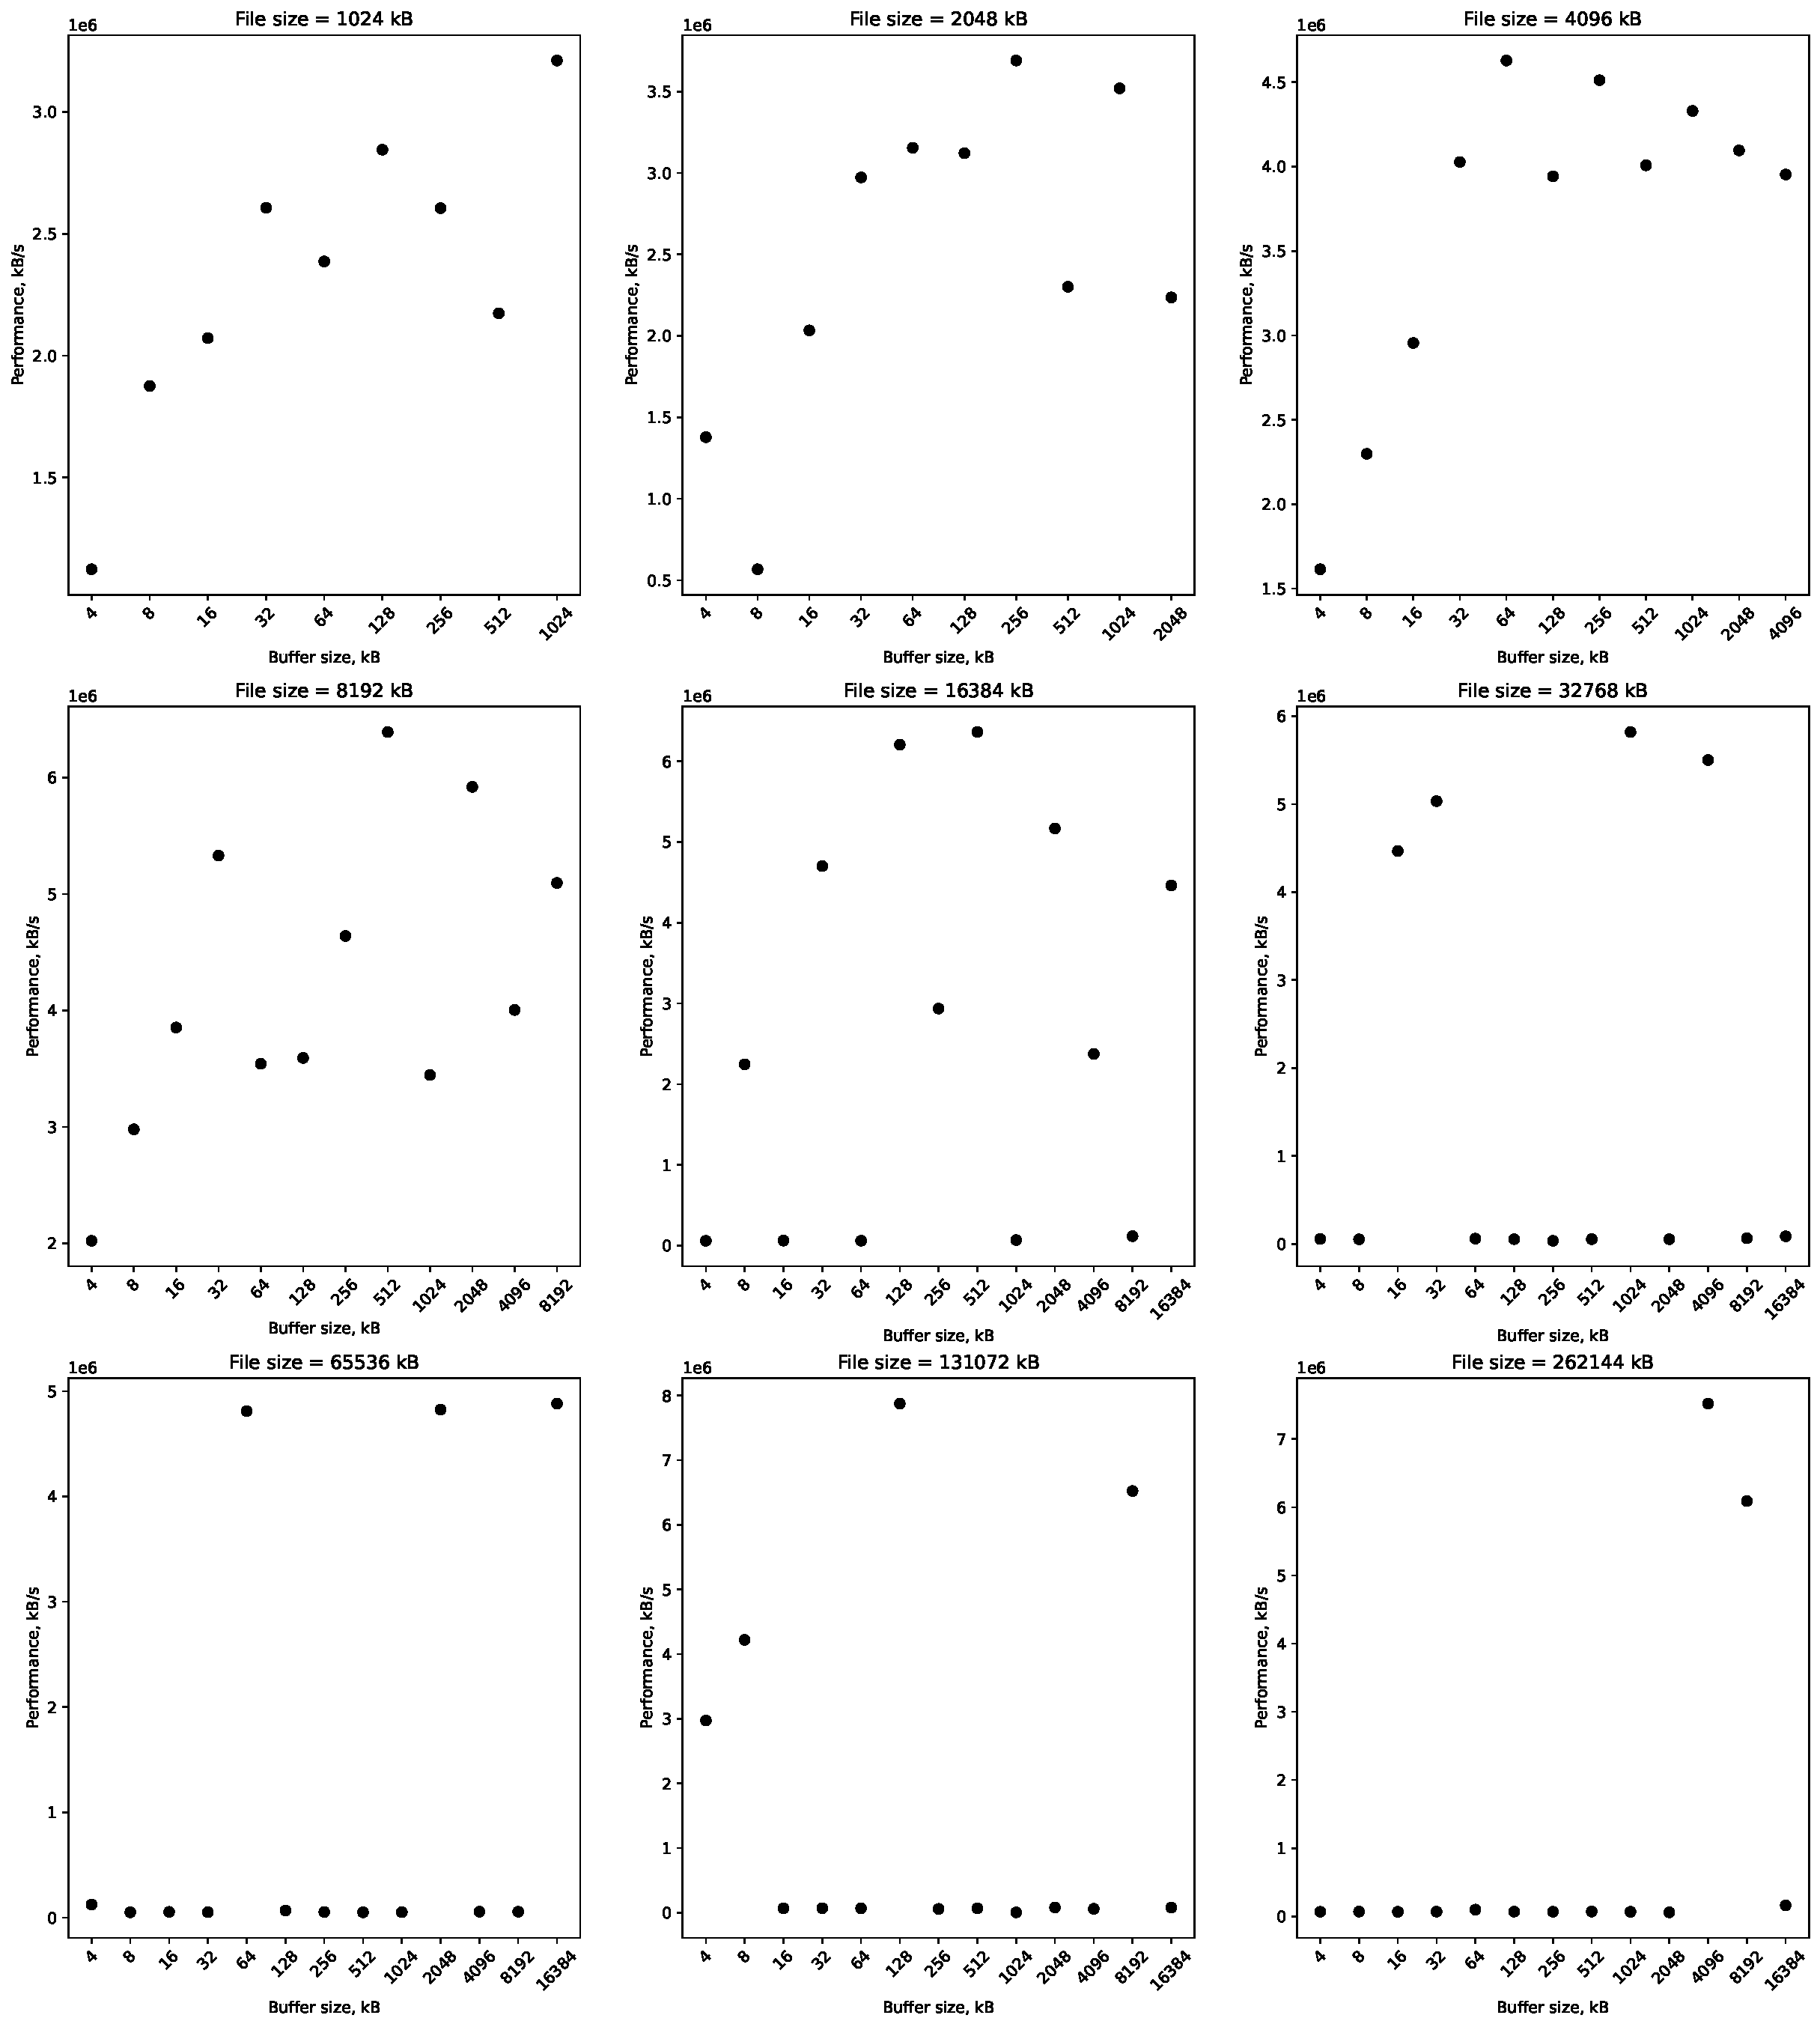
\includegraphics[width=1.0\textwidth]{figures/benchmarking/ffs/Read.pdf}
	\end{center}
	\caption{IOZone output for FFS Forward Read}
\end{figure}

\begin{figure}[!htb]
	\label{fig:app_bench_ffs_write}
	\begin{center}
		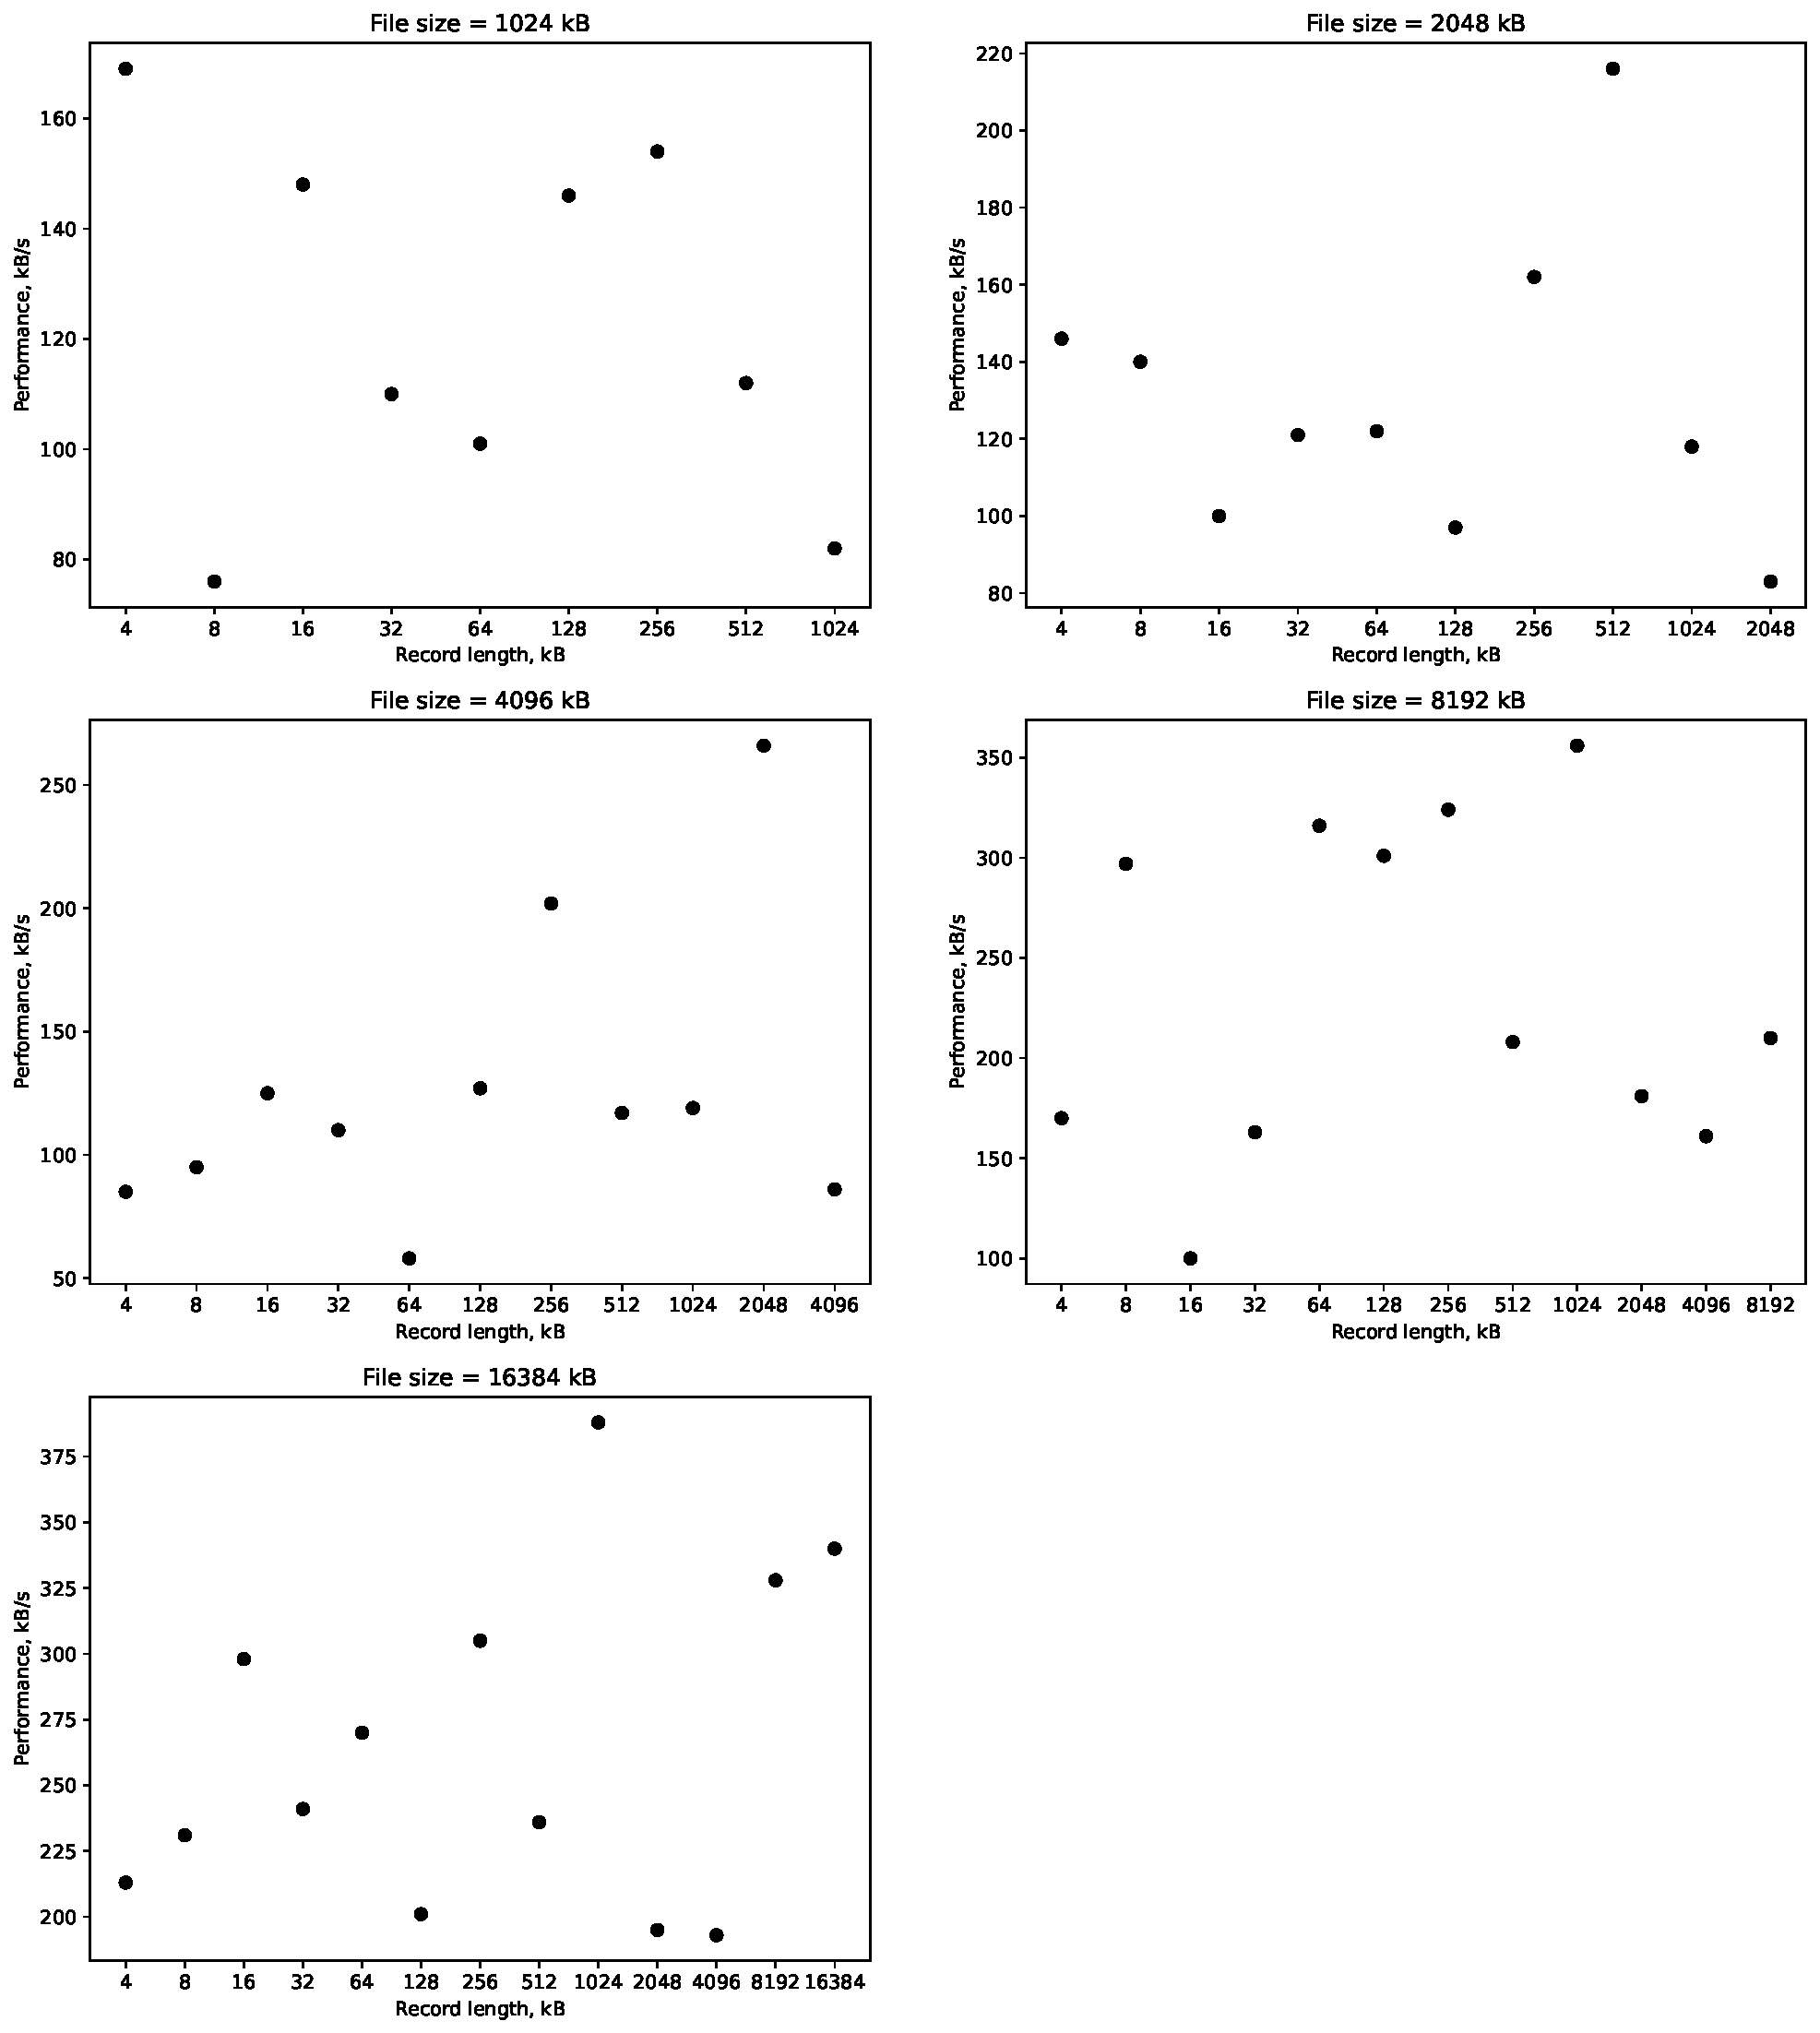
\includegraphics[width=1.0\textwidth]{figures/benchmarking/ffs/Write.pdf}
	\end{center}
	\caption{IOZone output for FFS Forward Write}
\end{figure}

\begin{figure}[!htb]
	\label{fig:app_bench_ffs_re_read}
	\begin{center}
		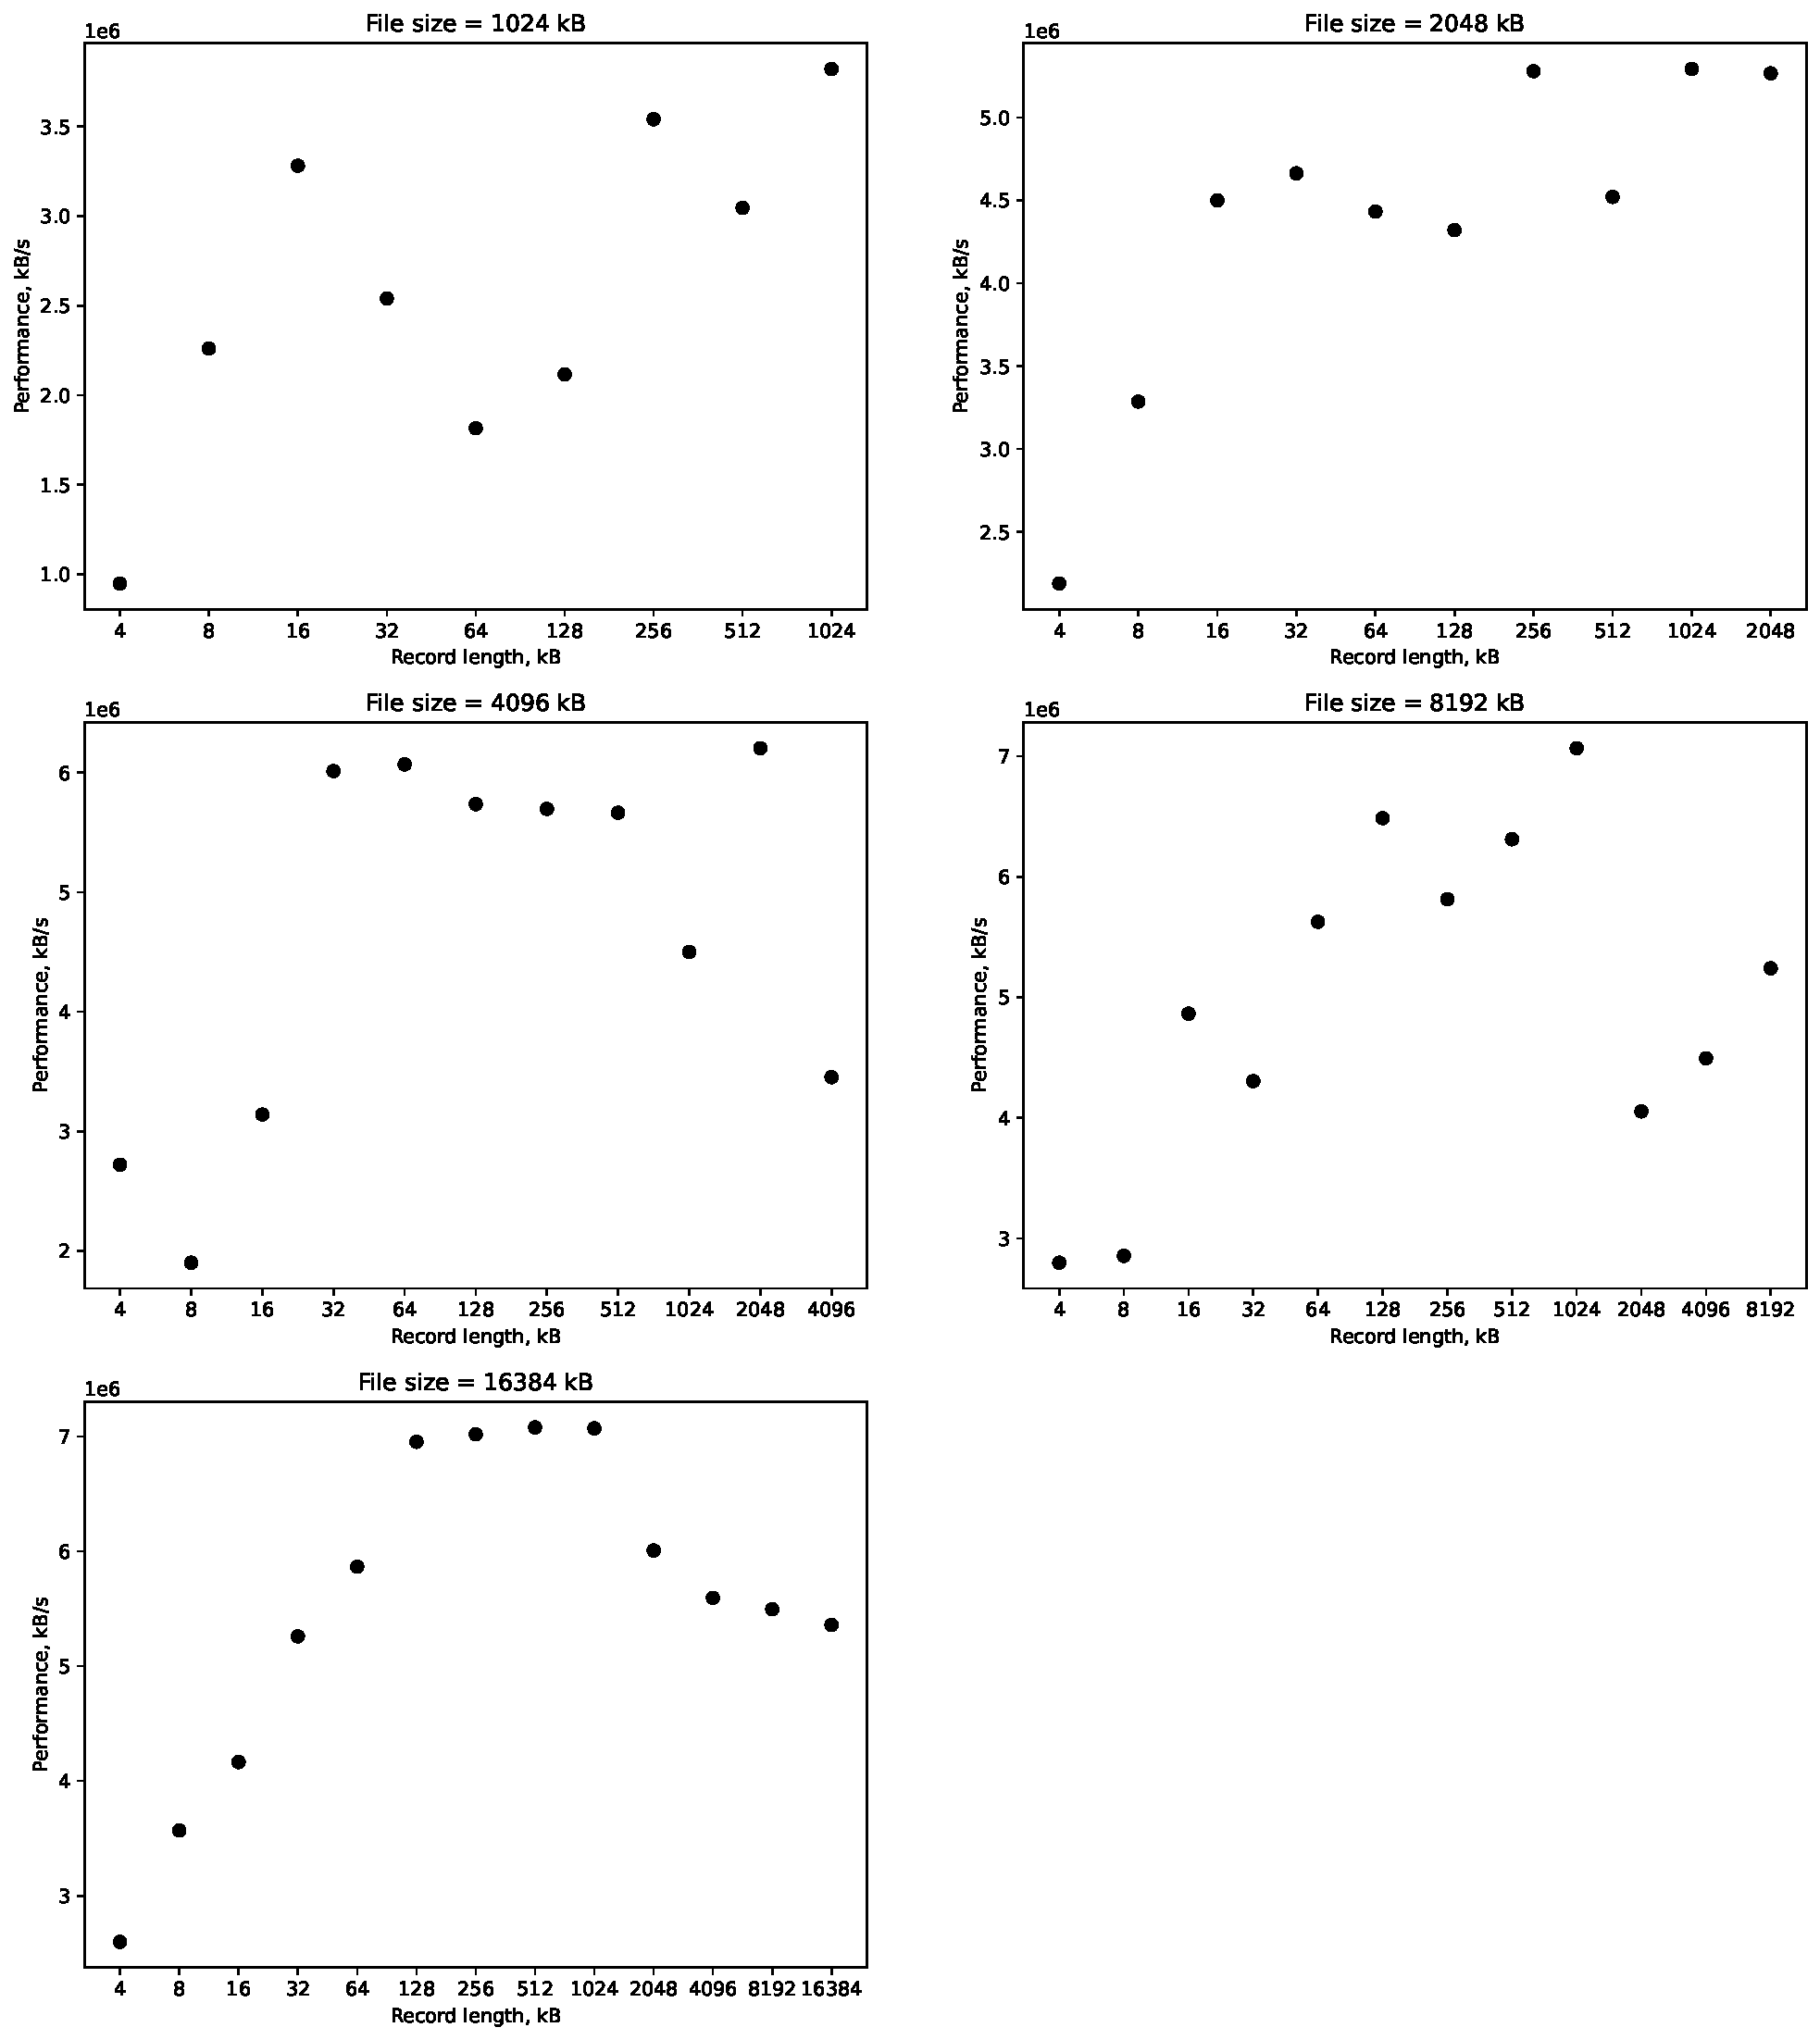
\includegraphics[width=1.0\textwidth]{figures/benchmarking/ffs/Re-Read.pdf}
	\end{center}
	\caption{IOZone output for FFS Re-Read}
\end{figure}

\begin{figure}[!htb]
	\label{fig:app_bench_ffs_re_write}
	\begin{center}
		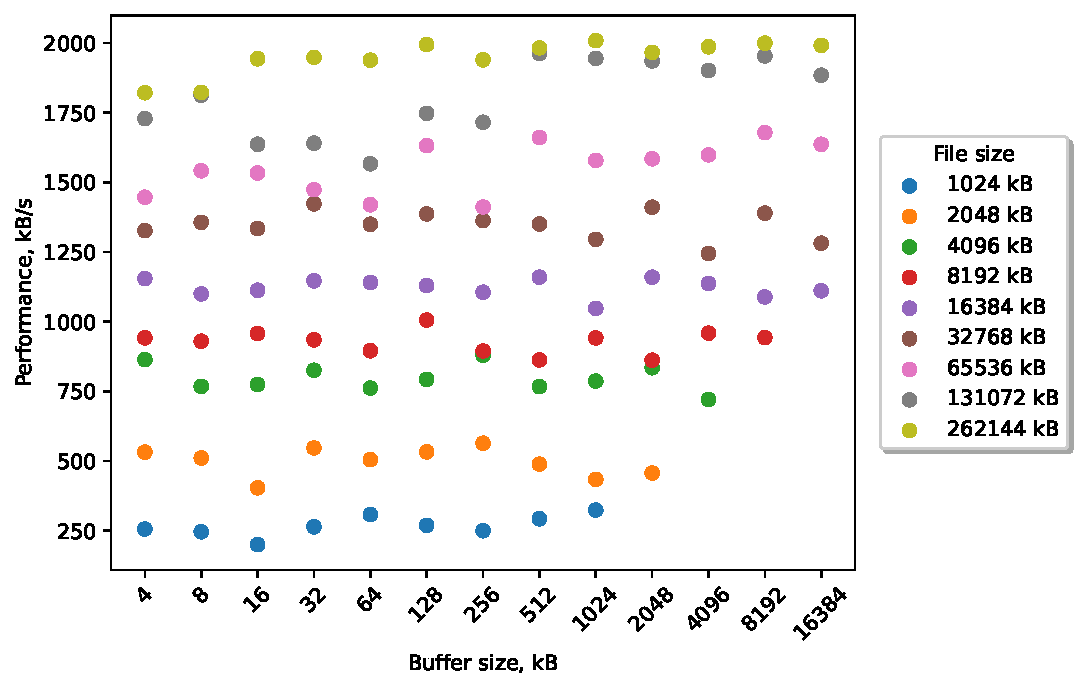
\includegraphics[width=1.0\textwidth]{figures/benchmarking/ffs/Re-Write.pdf}
	\end{center}
	\caption{IOZone output for FFS Re-Write}
\end{figure}

\begin{figure}[!htb]
	\label{fig:app_bench_ffs_rnd_read}
	\begin{center}
		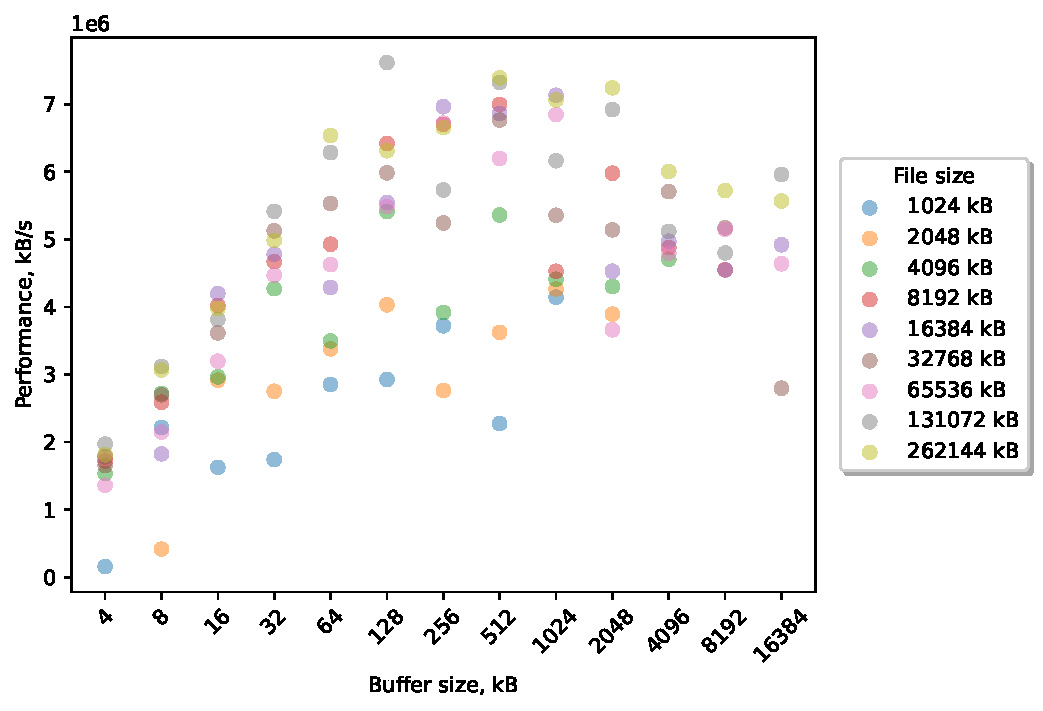
\includegraphics[width=1.0\textwidth]{figures/benchmarking/ffs/Random read.pdf}
	\end{center}
	\caption{IOZone output for FFS Random read}
\end{figure}

\begin{figure}[!htb]
	\label{fig:app_bench_ffs_rnd_write}
	\begin{center}
		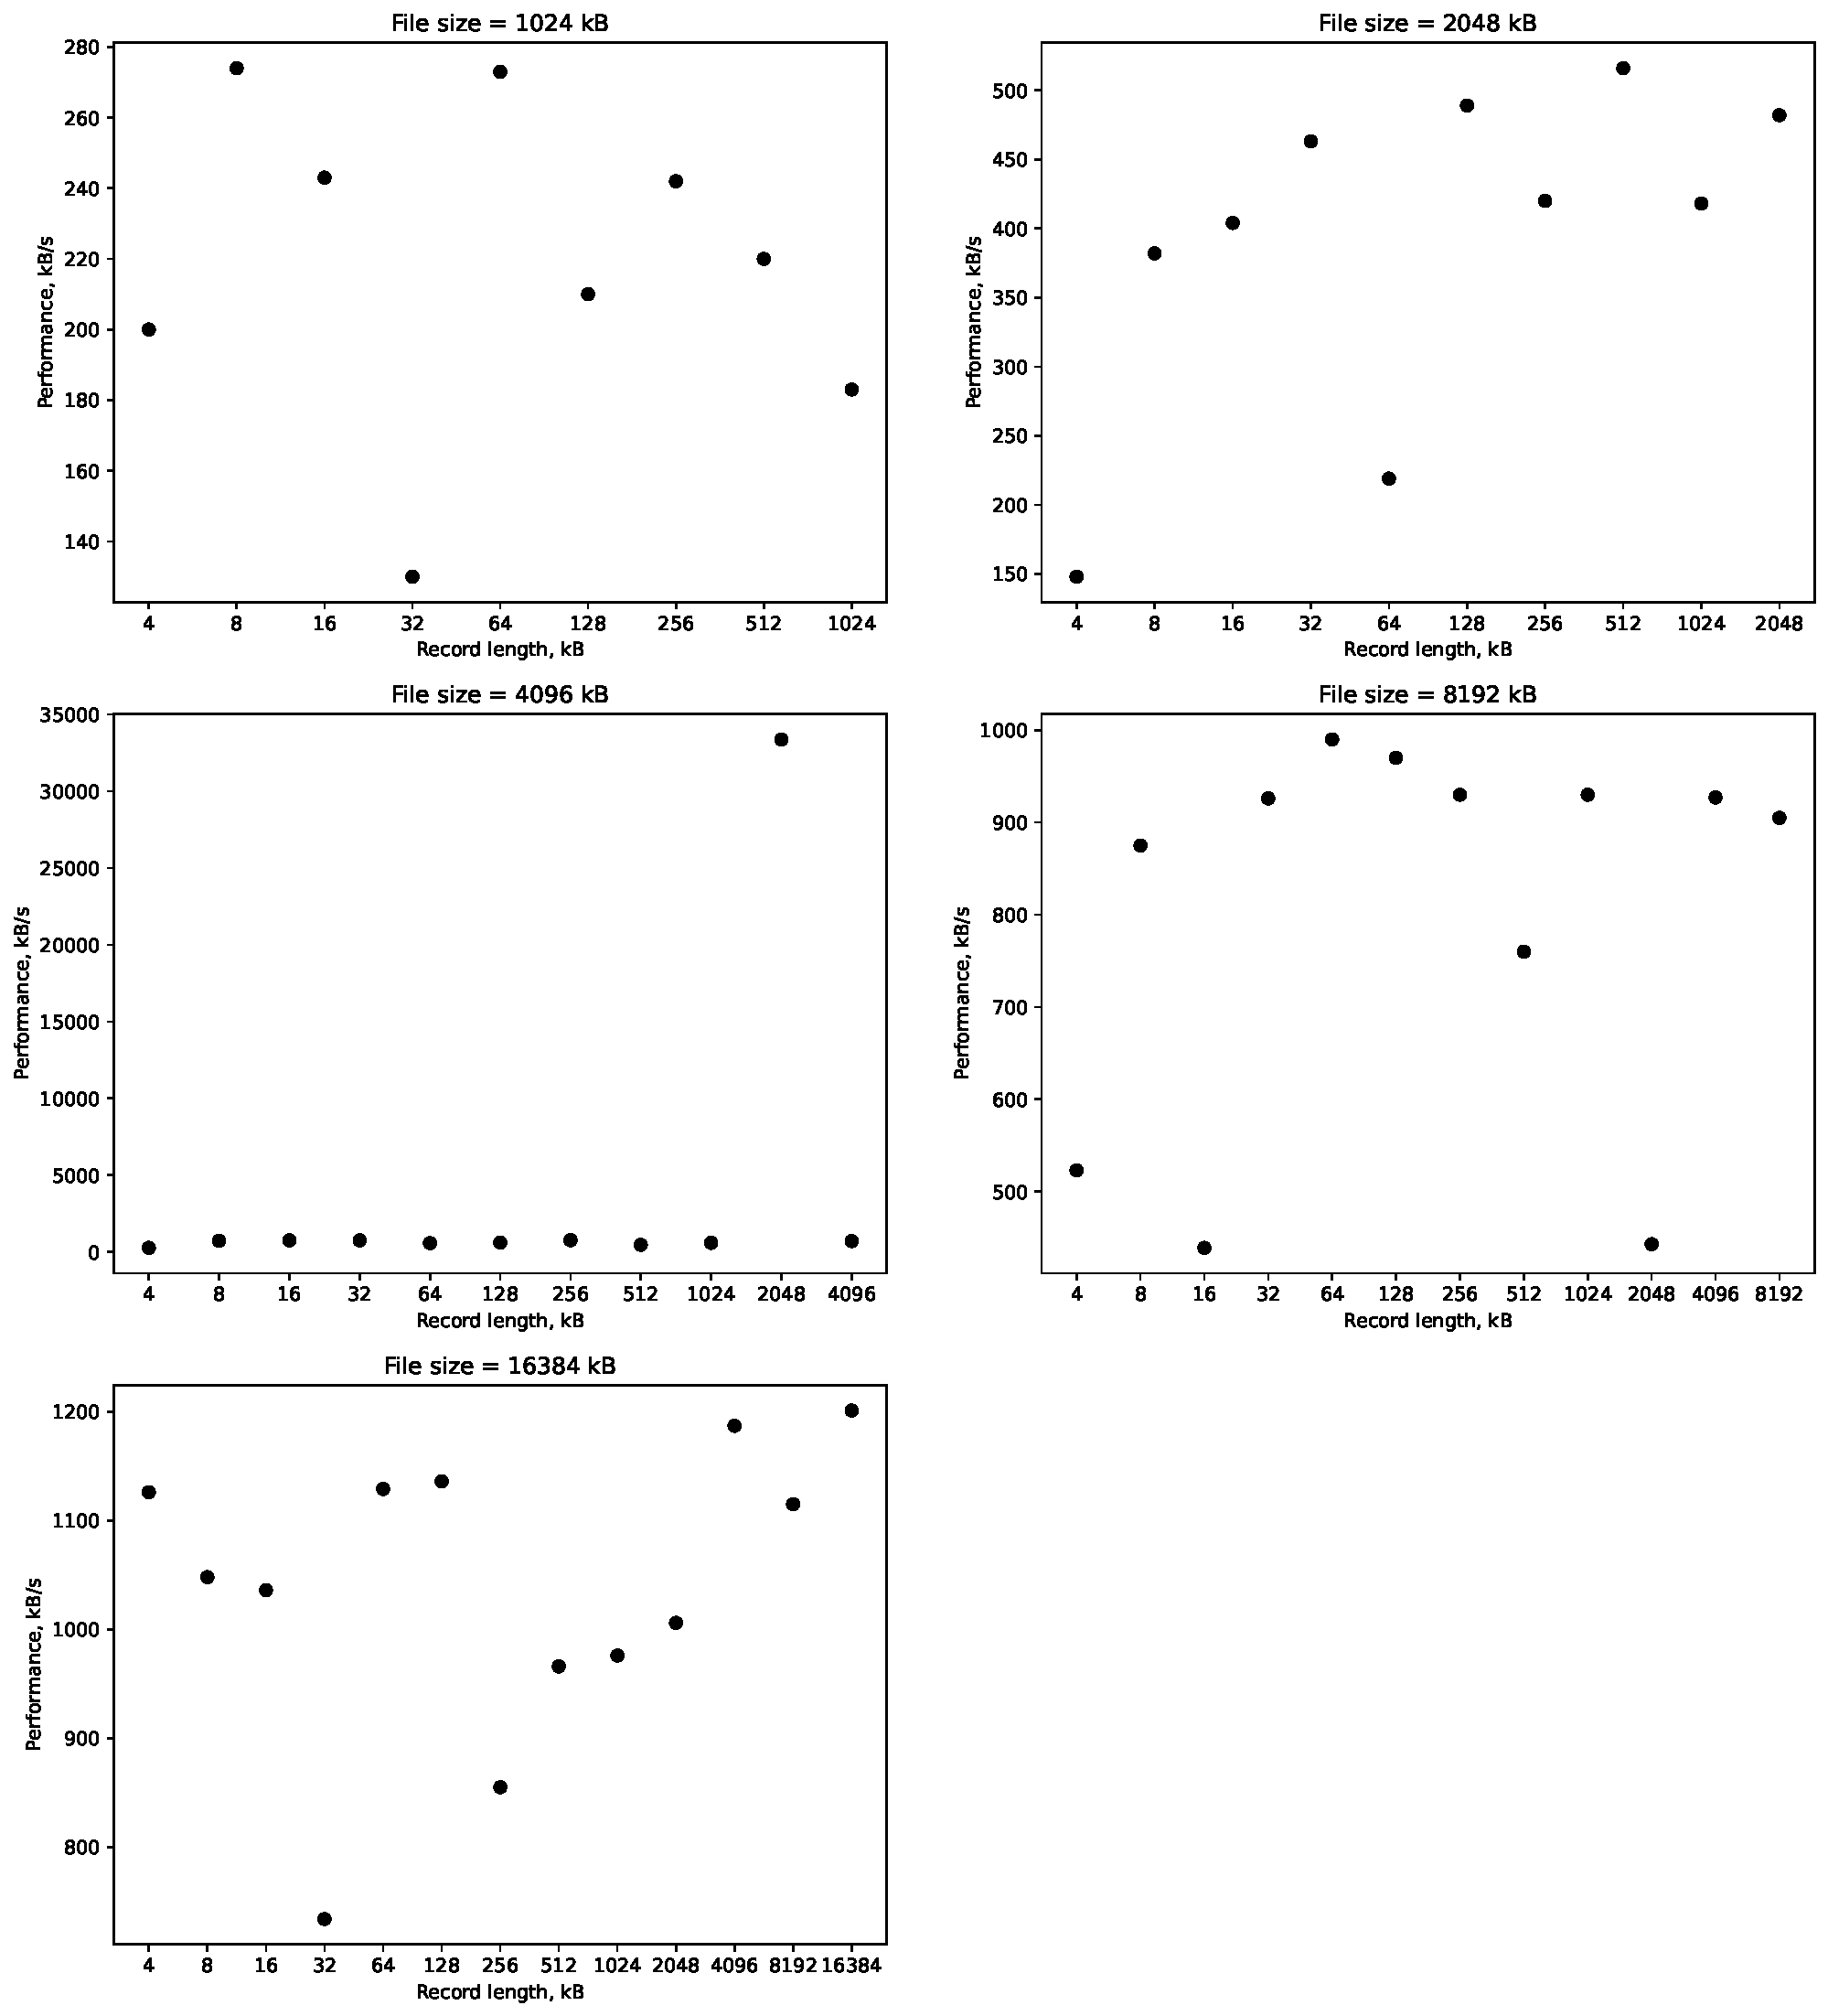
\includegraphics[width=1.0\textwidth]{figures/benchmarking/ffs/Random write.pdf}
	\end{center}
	\caption{IOZone output for FFS Random write}
\end{figure}

\section{GCSF}

\begin{table}[!ht]
	\begin{center}
		\caption{IOZone result for the Read test on GCSF in kilobytes per second}
		\resizebox{\textwidth}{!}{\begin{tabular}{| r | r | r | r | r | r | r | r | r | r | r | r | r | r | }
			
			\hline
			{} & \multicolumn{13}{c |}{Buffer size (kB)} \\
			\textbf{File size (kB)}   & \multicolumn{1}{c |}{4} & \multicolumn{1}{c |}{8} & \multicolumn{1}{c |}{16} & \multicolumn{1}{c |}{32} & \multicolumn{1}{c |}{64} & \multicolumn{1}{c |}{128} & \multicolumn{1}{c |}{256} & \multicolumn{1}{c |}{512} & \multicolumn{1}{c |}{1024} & \multicolumn{1}{c |}{2048} & \multicolumn{1}{c |}{4096} & \multicolumn{1}{c |}{8192} & \multicolumn{1}{c |}{16384}\\
			\hline
			\hline
			\textbf{1024}  & 1790460 & 2035716 & 2753527 & 3411938 & 3003881 & 3401130 & 3722435 & 4162573 & 4493556 & {} & {} & {} & {}\\
			\textbf{2048}  & 945007 & 2308622 & 3297725 & 4170264 & 3698085 & 2467800 & 3506373 & 4611288 & 5416763 & 4376355 & {} & {} & {}\\
			\textbf{4096}  & 1858527 & 2813233 & 1017897 & 4969868 & 4399673 & 4941279 & 4591331 & 5657217 & 5625724 & 5019235 & 3327622 & {} & {}\\
			\textbf{8192}  & 651866 & 480214 & 4126896 & 4664763 & 903994 & 5357988 & 3195123 & 5288712 & 6804170 & 1412655 & 4833405 & 5085204 & {}\\
			\textbf{16384}  & 409261 & 3463891 & 4768276 & 518677 & 5797739 & 6450228 & 6077171 & 6143453 & 6930296 & 6316241 & 5948808 & 837411 & 5326345\\
			\textbf{32768}  & 289995 & 2604351 & 514007 & 5222875 & 351689 & 380969 & 225834 & 428160 & 377558 & 3011251 & 422812 & 601160 & 710955\\
			\textbf{65536}  & 420968 & 390311 & 374191 & 590919 & 6243421 & 863782 & 388813 & 506734 & 463735 & 478777 & 456922 & 429282 & 624033\\
			\textbf{131072}  & 443068 & 462364 & 407350 & 496836 & 444001 & 471616 & 424145 & 518826 & 505112 & 559713 & 375452 & 526586 & 515828\\


			\hline

		\end{tabular}}
		\label{tbl:data_gcsf_read}
	\end{center}
\end{table}
	
\begin{table}[!ht]
	\begin{center}
		\caption{IOZone result for the Write test on GCSF in kilobytes per second}
		\resizebox{\textwidth}{!}{\begin{tabular}{| r | r | r | r | r | r | r | r | r | r | r | r | r | r | }
			
			\hline
			{} & \multicolumn{13}{c |}{Buffer size (kB)} \\
			\textbf{File size (kB)}   & \multicolumn{1}{c |}{4} & \multicolumn{1}{c |}{8} & \multicolumn{1}{c |}{16} & \multicolumn{1}{c |}{32} & \multicolumn{1}{c |}{64} & \multicolumn{1}{c |}{128} & \multicolumn{1}{c |}{256} & \multicolumn{1}{c |}{512} & \multicolumn{1}{c |}{1024} & \multicolumn{1}{c |}{2048} & \multicolumn{1}{c |}{4096} & \multicolumn{1}{c |}{8192} & \multicolumn{1}{c |}{16384}\\
			\hline
			\hline
			\textbf{1024}  & 489 & 517 & 445 & 461 & 399 & 496 & 509 & 448 & 529 & {} & {} & {} & {}\\
			\textbf{2048}  & 937 & 966 & 854 & 944 & 1072 & 966 & 944 & 954 & 868 & 969 & {} & {} & {}\\
			\textbf{4096}  & 1609 & 1614 & 1749 & 1607 & 1213 & 1787 & 1802 & 1519 & 1748 & 1551 & 1784 & {} & {}\\
			\textbf{8192}  & 3047 & 2233 & 2746 & 3115 & 2666 & 2636 & 3000 & 2974 & 3165 & 2716 & 3138 & 3122 & {}\\
			\textbf{16384}  & 4372 & 4180 & 4437 & 4690 & 4798 & 4642 & 4429 & 4781 & 4705 & 4670 & 4621 & 4875 & 4607\\
			\textbf{32768}  & 5377 & 6125 & 6471 & 6402 & 6343 & 6463 & 6435 & 6289 & 5865 & 6052 & 6317 & 6291 & 6018\\
			\textbf{65536}  & 6763 & 7448 & 7298 & 7825 & 6561 & 7061 & 7818 & 6959 & 7491 & 7706 & 5985 & 7343 & 6851\\
			\textbf{131072}  & 7276 & 7789 & 8553 & 8609 & 8243 & 8596 & 8168 & 8530 & 8596 & 8433 & 8029 & 8280 & 7959\\


			\hline

		\end{tabular}}
		\label{tbl:data_gcsf_write}
	\end{center}
\end{table}
	
\begin{table}[!ht]
	\begin{center}
		\caption{IOZone result for the Re-Read test on GCSF}
		\resizebox{\textwidth}{!}{\begin{tabular}{| c | c | c | c | c | c | c | c | c | c | c | c | c | c | }
			
			\hline
			{} & \multicolumn{13}{c |}{Buffer size (kB)} \\
			\textbf{File size (kB)}   & 4 & 8 & 16 & 32 & 64 & 128 & 256 & 512 & 1024 & 2048 & 4096 & 8192 & 16384\\
			\hline
			\hline
			\textbf{1024}  & 2632033 & 2187063 & 3200886 & 4304412 & 3348104 & 3778101 & 3281592 & 5048117 & 4083422 & {} & {} & {} & {}\\
			\textbf{2048}  & 2311728 & 3261415 & 4623699 & 4643695 & 4079167 & 4349761 & 6149699 & 6058611 & 7213548 & 5032754 & {} & {} & {}\\
			\textbf{4096}  & 2356697 & 2579635 & 4329816 & 5424983 & 5347310 & 6309619 & 4371684 & 6585338 & 6894546 & 6370451 & 5165626 & {} & {}\\
			\textbf{8192}  & 1891555 & 3974610 & 4017834 & 4884942 & 6112956 & 6262248 & 5158495 & 5116249 & 7087688 & 6720329 & 5270864 & 5038228 & {}\\
			\textbf{16384}  & 2228199 & 3960364 & 5075741 & 6187150 & 6473317 & 6838571 & 6919132 & 7139088 & 7211005 & 6614761 & 6187707 & 5016457 & 4594528\\
			\textbf{32768}  & 2503678 & 3836954 & 4593731 & 6020418 & 6336861 & 5357031 & 1864671 & 6139832 & 5652480 & 6276093 & 5945927 & 4010262 & 4741431\\
			\textbf{65536}  & 2639381 & 3531600 & 5031555 & 6133503 & 6445904 & 5921182 & 5961505 & 6217859 & 6461207 & 6398788 & 5278722 & 4674094 & 5364747\\
			\textbf{131072}  & 3039494 & 3904216 & 4889073 & 5950781 & 6275836 & 7495395 & 5875292 & 7344197 & 7196622 & 8031869 & 4689156 & 5687415 & 5207460\\


			\hline

		\end{tabular}}
		\label{tbl:data_gcsf_re-read}
	\end{center}
\end{table}
	
\begin{table}[!ht]
	\begin{center}
		\caption{IOZone result for GCSF Re-Write}
		\resizebox{\textwidth}{!}{\begin{tabular}{| c | c | c | c | c | c | c | c | c | c | c | c | c | c | }
			
			\hline
			{} & \multicolumn{13}{c |}{Buffer size (kB)} \\
			\textbf{File size (kB)}   & 4 & 8 & 16 & 32 & 64 & 128 & 256 & 512 & 1024 & 2048 & 4096 & 8192 & 16384\\
			\hline
			\hline
			\textbf{1024}  & 352 & 201 & 409 & 412 & 487 & 420 & 200 & 442 & 438 & {} & {} & {} & {}\\
			\textbf{2048}  & 600 & 765 & 625 & 759 & 731 & 722 & 663 & 742 & 703 & 718 & {} & {} & {}\\
			\textbf{4096}  & 934 & 1100 & 795 & 762 & 1295 & 1501 & 1421 & 1424 & 1444 & 1423 & 1209 & {} & {}\\
			\textbf{8192}  & 293 & 1197 & 318 & 602 & 2306 & 2086 & 2254 & 2239 & 2247 & 2201 & 2252 & 2200 & {}\\
			\textbf{16384}  & 1420 & 1472 & 1264 & 1563 & 695 & 2986 & 2074 & 2996 & 3126 & 3033 & 2649 & 3000 & 2890\\


			\hline

		\end{tabular}}
		\label{tbl:data_re-write_gcsf}
	\end{center}
\end{table}
	
\begin{table}[!ht]
	\begin{center}
		\caption{IOZone result for the Random read test on GCSF}
		\resizebox{\textwidth}{!}{\begin{tabular}{| c | c | c | c | c | c | c | c | c | c | c | c | c | c | }
			
			\hline
			{} & \multicolumn{13}{c |}{Buffer size (kB)} \\
			\textbf{File size (kB)}   & 4 & 8 & 16 & 32 & 64 & 128 & 256 & 512 & 1024 & 2048 & 4096 & 8192 & 16384\\
			\hline
			\hline
			\textbf{1024}  & 1992279 & 1741104 & 3923040 & 2892612 & 3284101 & 2875184 & 4282950 & 3684119 & 3179559 & {} & {} & {} & {}\\
			\textbf{2048}  & 2122645 & 2592166 & 2843590 & 5006356 & 4221501 & 4481379 & 6583305 & 5200329 & 7343043 & 4934459 & {} & {} & {}\\
			\textbf{4096}  & 1723189 & 2471992 & 4007615 & 4899008 & 5625724 & 5713661 & 6503078 & 6897314 & 4958393 & 5270212 & 5063617 & {} & {}\\
			\textbf{8192}  & 1438199 & 3111222 & 4149824 & 5095007 & 5821902 & 5885728 & 4543853 & 6350207 & 7173514 & 6501608 & 5372229 & 4654652 & {}\\
			\textbf{16384}  & 1859705 & 2912112 & 4175240 & 5158807 & 6039252 & 6725463 & 6203907 & 6921919 & 6820923 & 6546080 & 5667676 & 5441055 & 5336686\\
			\textbf{32768}  & 1705159 & 2794224 & 4285618 & 5467855 & 5548200 & 6087347 & 6091664 & 5991547 & 5893405 & 6215636 & 6222672 & 3776853 & 5156254\\
			\textbf{65536}  & 1843064 & 2695626 & 4393982 & 4975003 & 6203125 & 5990477 & 4676082 & 7062855 & 6735419 & 6700285 & 4143421 & 4907587 & 5587993\\
			\textbf{131072}  & 2100647 & 2842719 & 3678063 & 5056629 & 5706720 & 6765741 & 5708261 & 7233171 & 7090347 & 7451506 & 4198987 & 5471360 & 5404768\\


			\hline

		\end{tabular}}
		\label{tbl:data_gcsf_random_read}
	\end{center}
\end{table}
	
\begin{table}[!ht]
	\begin{center}
		\caption{IOZone result for GCSF Random write}
		\resizebox{\textwidth}{!}{\begin{tabular}{| c | c | c | c | c | c | c | c | c | c | c | c | c | c | }
			
			\hline
			{} & \multicolumn{13}{c |}{Buffer size (kB)} \\
			\textbf{File size (kB)}   & 4 & 8 & 16 & 32 & 64 & 128 & 256 & 512 & 1024 & 2048 & 4096 & 8192 & 16384\\
			\hline
			\hline
			\textbf{1024}  & 451 & 261 & 394 & 439 & 383 & 383 & 372 & 224 & 466 & {} & {} & {} & {}\\
			\textbf{2048}  & 687 & 811 & 785 & 808 & 715 & 632 & 712 & 798 & 805 & 564 & {} & {} & {}\\
			\textbf{4096}  & 888 & 1337 & 1459 & 1363 & 1440 & 1323 & 1403 & 1473 & 1099 & 1426 & 1231 & {} & {}\\
			\textbf{8192}  & 2208 & 865 & 2220 & 2293 & 2177 & 2227 & 2213 & 2120 & 2151 & 2233 & 2207 & 2130 & {}\\
			\textbf{16384}  & 1282 & 1357 & 1560 & 3266 & 3523 & 2971 & 2604 & 2931 & 3001 & 3044 & 2973 & 3090 & 1270\\


			\hline

		\end{tabular}}
		\label{tbl:data_random_write_gcsf}
	\end{center}
\end{table}
	

\begin{figure}[!htb]
	\label{fig:app_bgcsfh_ffs_read}
	\begin{center}
		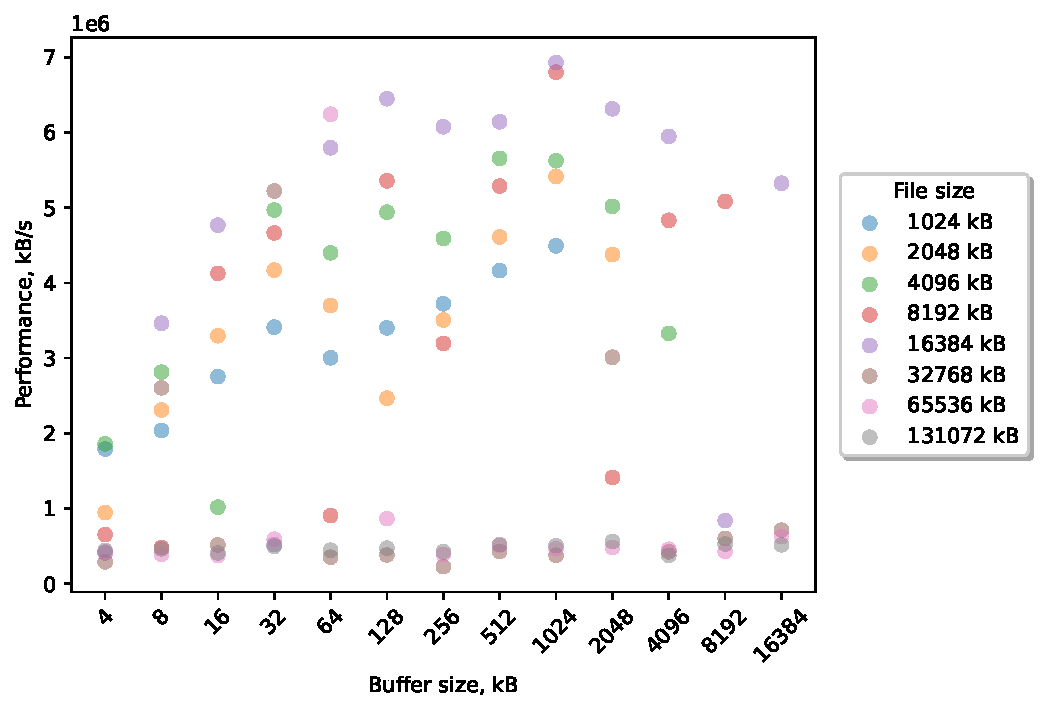
\includegraphics[width=1.0\textwidth]{figures/benchmarking/gcsf/Read.pdf}
	\end{center}
	\caption{IOZone output for GCSF Forward Read}
\end{figure}

\begin{figure}[!htb]
	\label{fig:app_begcsf_ffs_write}
	\begin{center}
		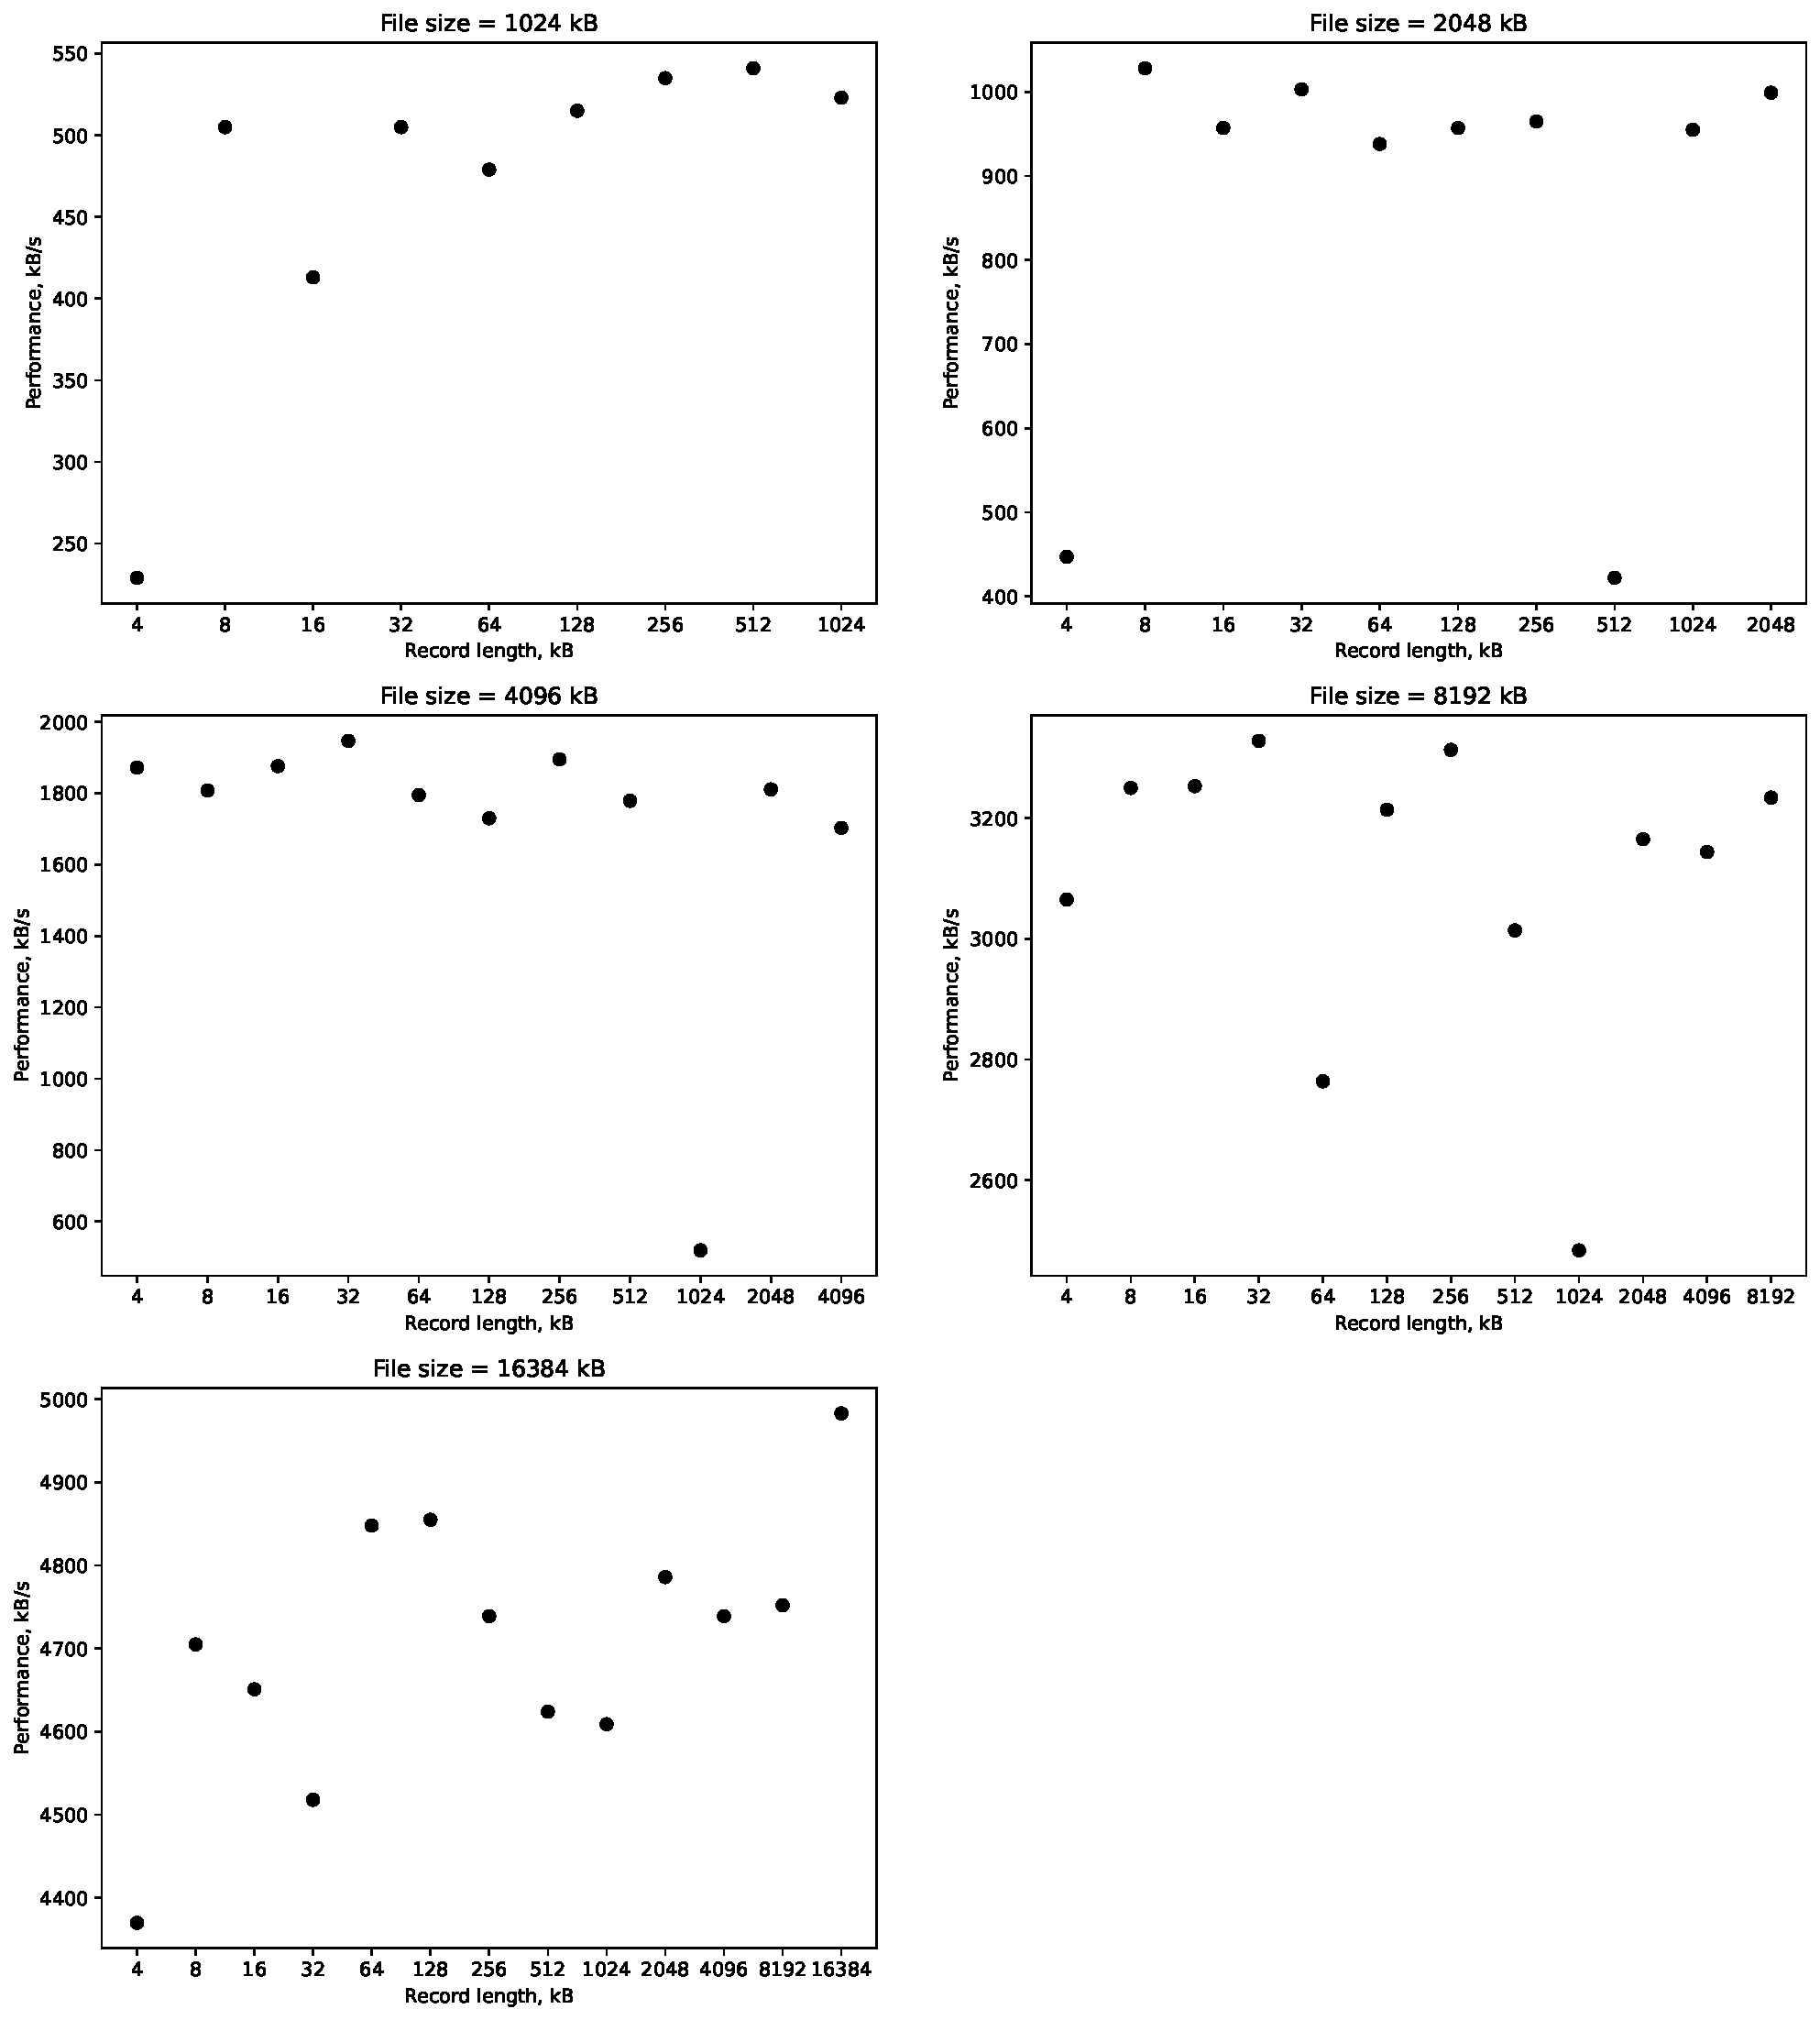
\includegraphics[width=1.0\textwidth]{figures/benchmarking/gcsf/Write.pdf}
	\end{center}
	\caption{IOZone output for GCSF Forward Write}
\end{figure}

\begin{figure}[!htb]
	\label{fig:app_bencgcsffs_re_read}
	\begin{center}
		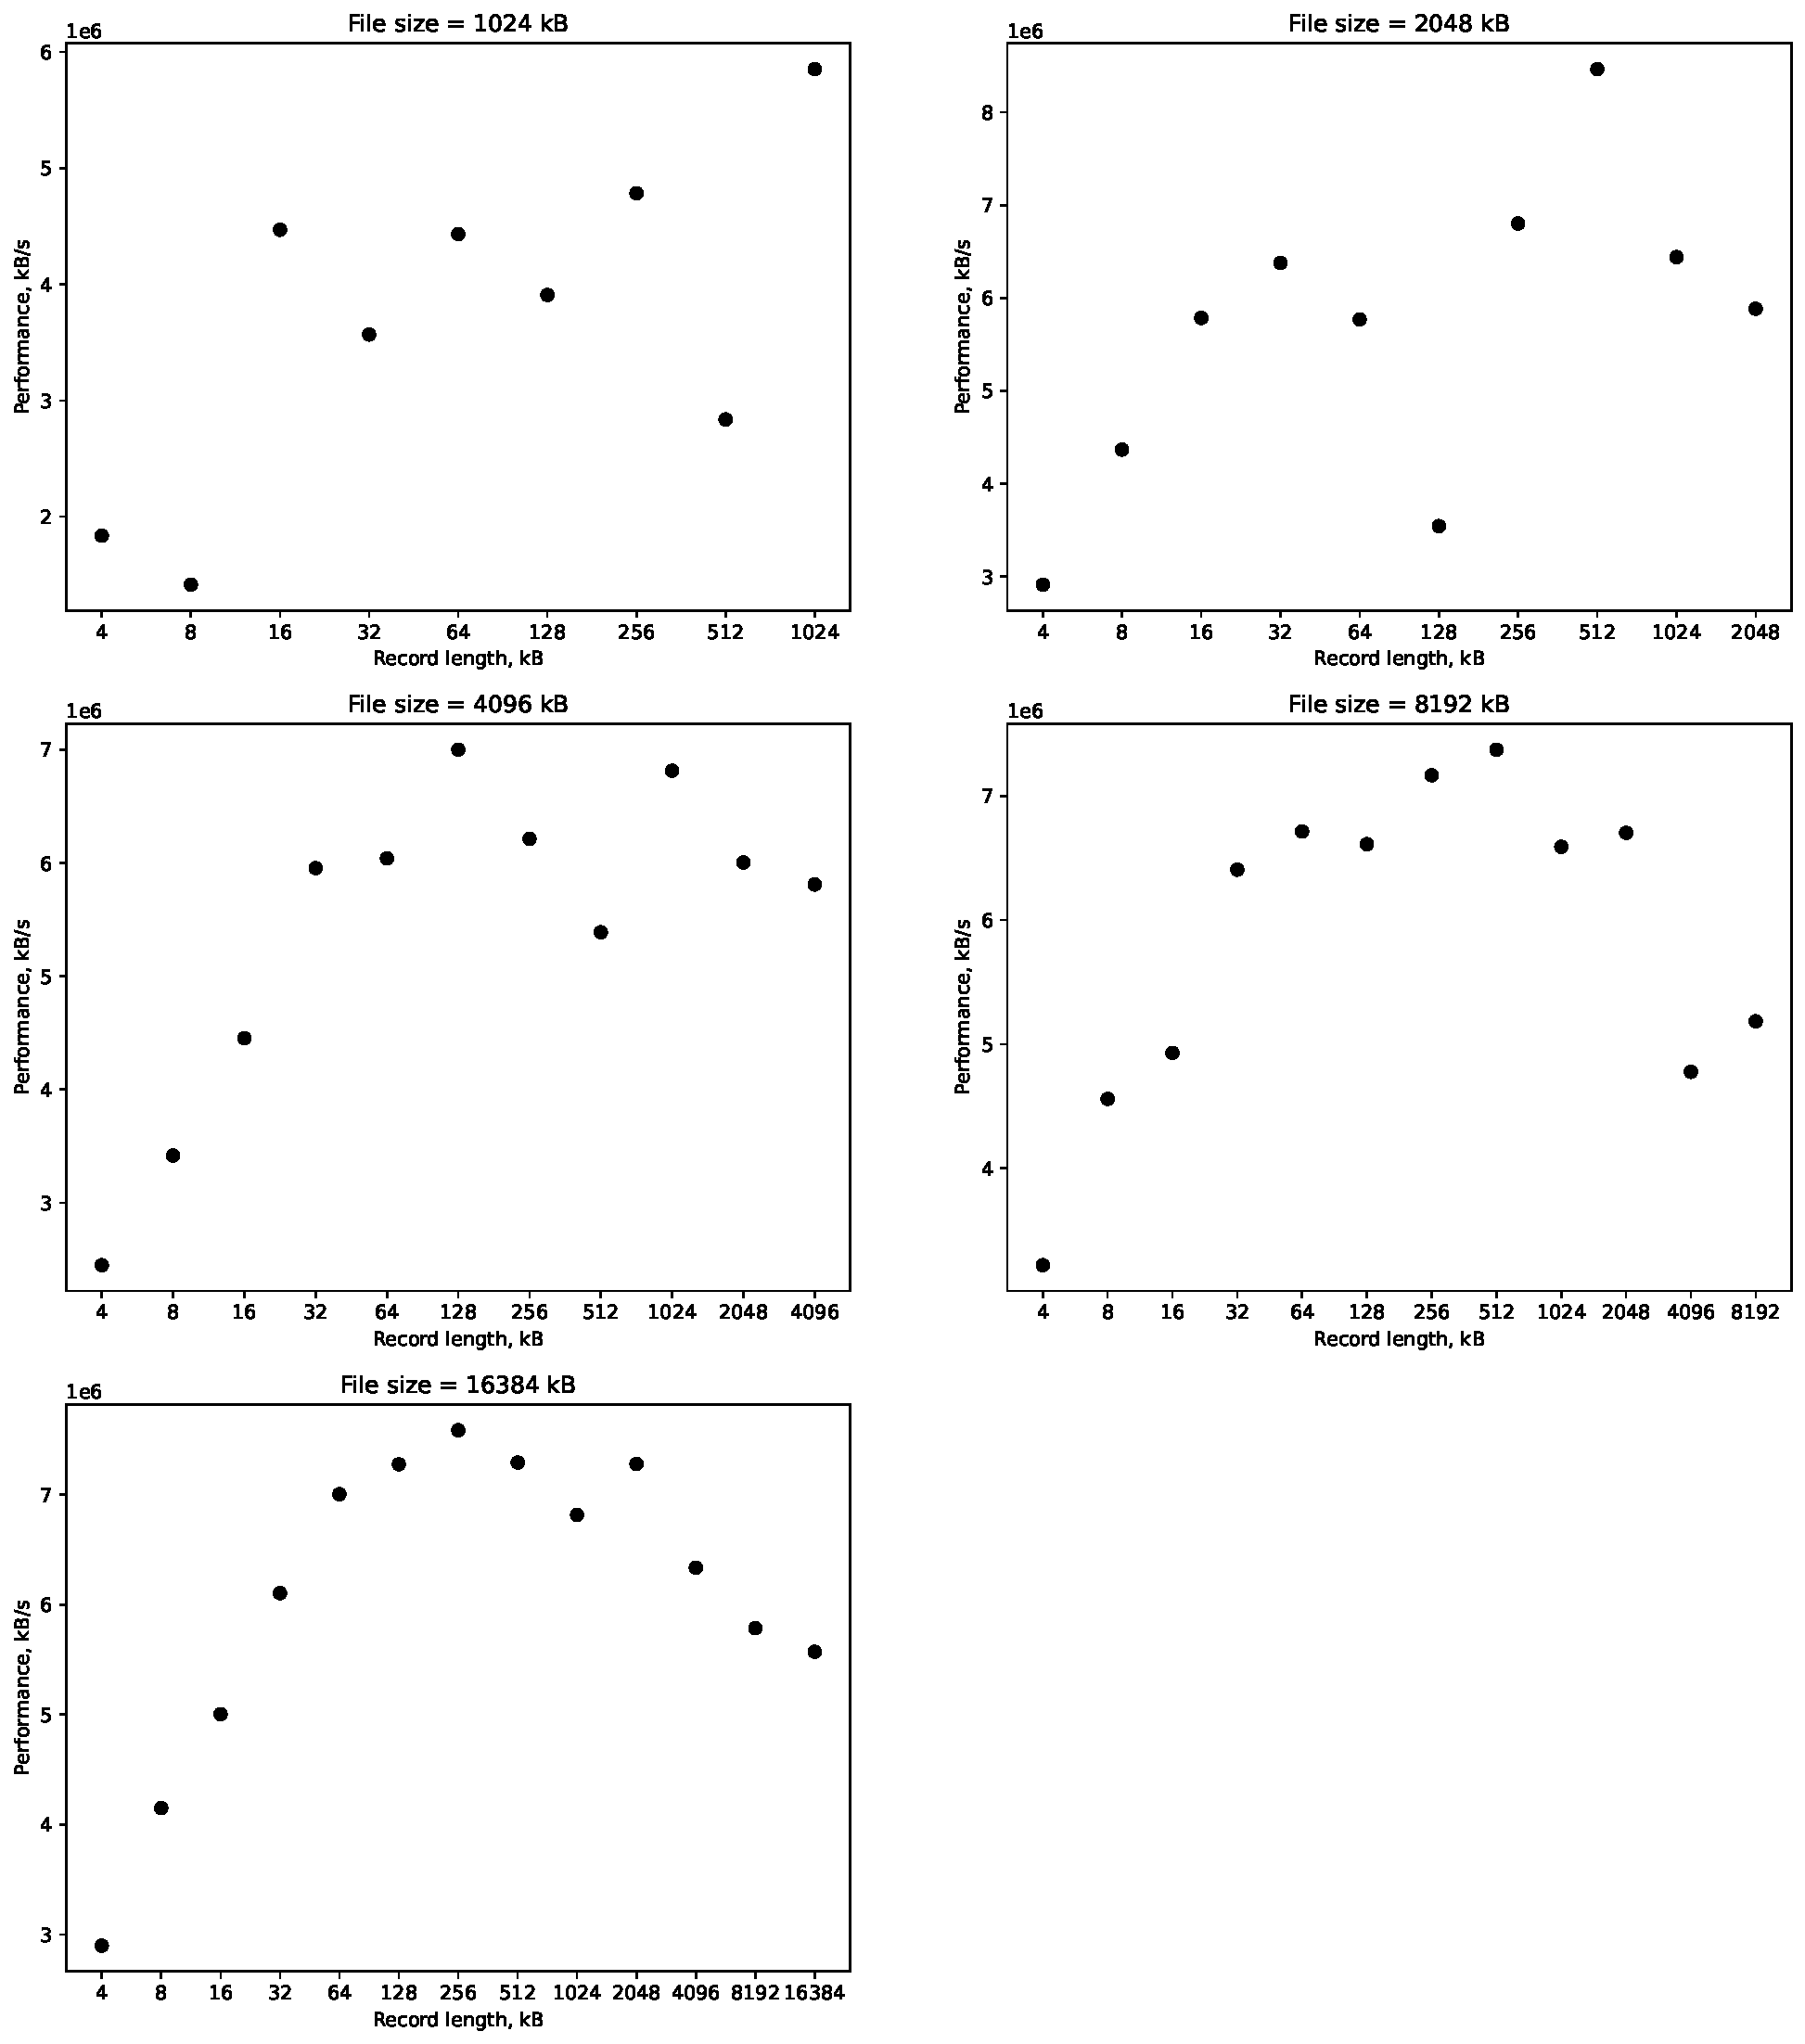
\includegraphics[width=1.0\textwidth]{figures/benchmarking/gcsf/Re-Read.pdf}
	\end{center}
	\caption{IOZone output for GCSF Re-Read}
\end{figure}

\begin{figure}[!htb]
	\label{fig:app_benchgcsfs_re_write}
	\begin{center}
		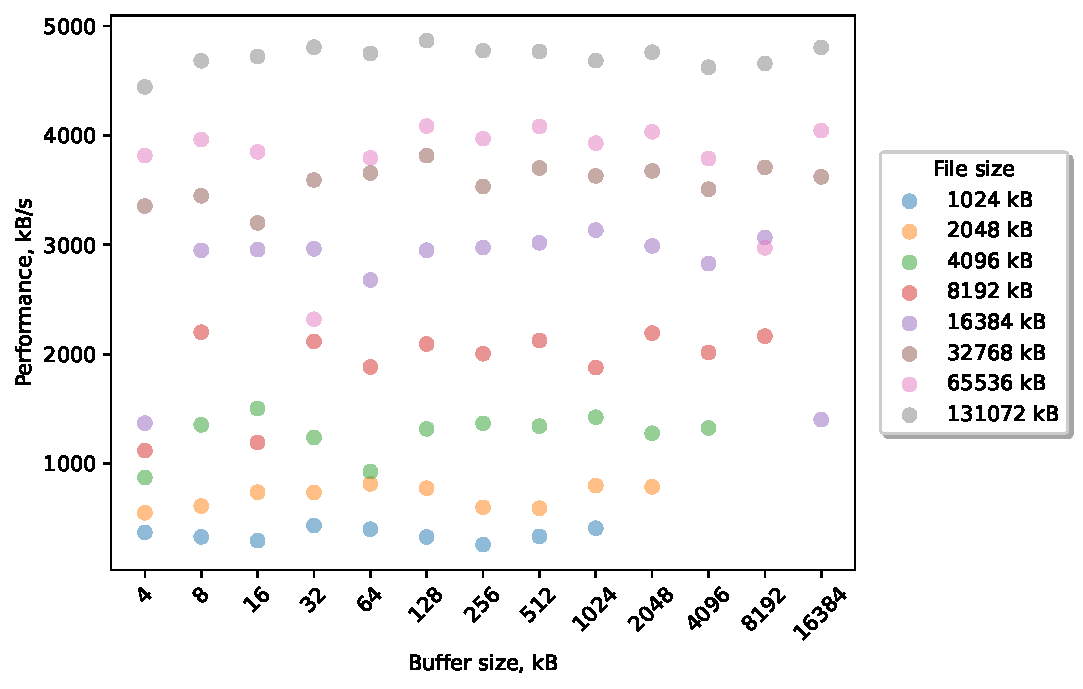
\includegraphics[width=1.0\textwidth]{figures/benchmarking/gcsf/Re-Write.pdf}
	\end{center}
	\caption{IOZone output for GCSF Re-Write}
\end{figure}

\begin{figure}[!htb]
	\label{fig:app_benchgcsfs_rnd_read}
	\begin{center}
		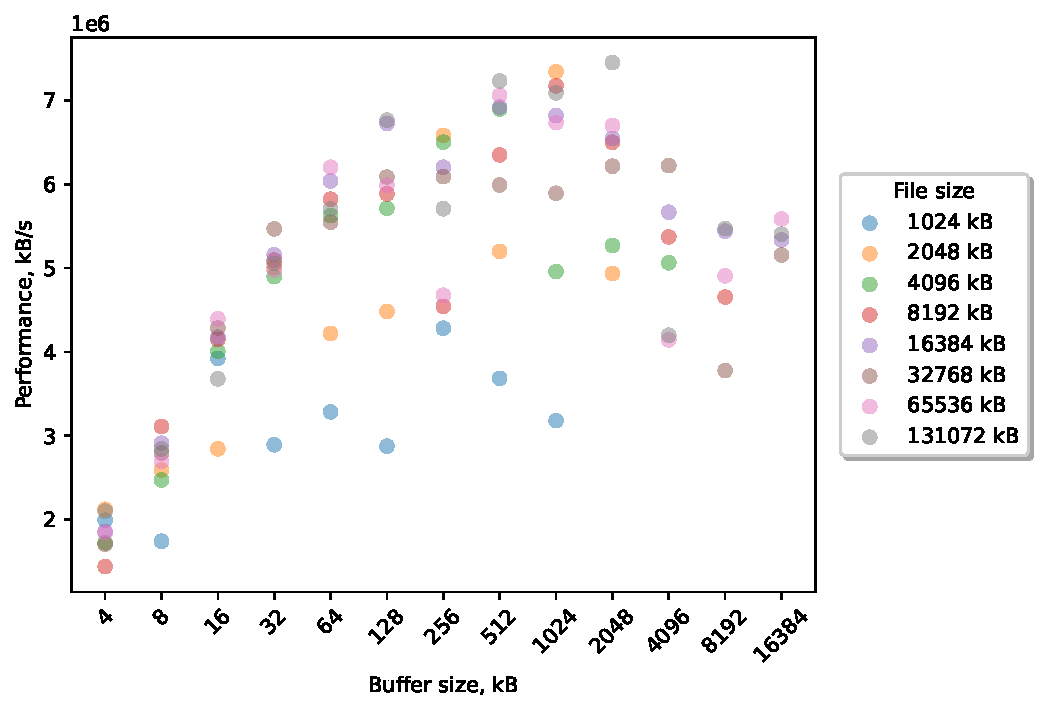
\includegraphics[width=1.0\textwidth]{figures/benchmarking/gcsf/Random read.pdf}
	\end{center}
	\caption{IOZone output for GCSF Random read}
\end{figure}

\begin{figure}[!htb]
	\label{fig:app_bench_gcsf_rnd_write}
	\begin{center}
		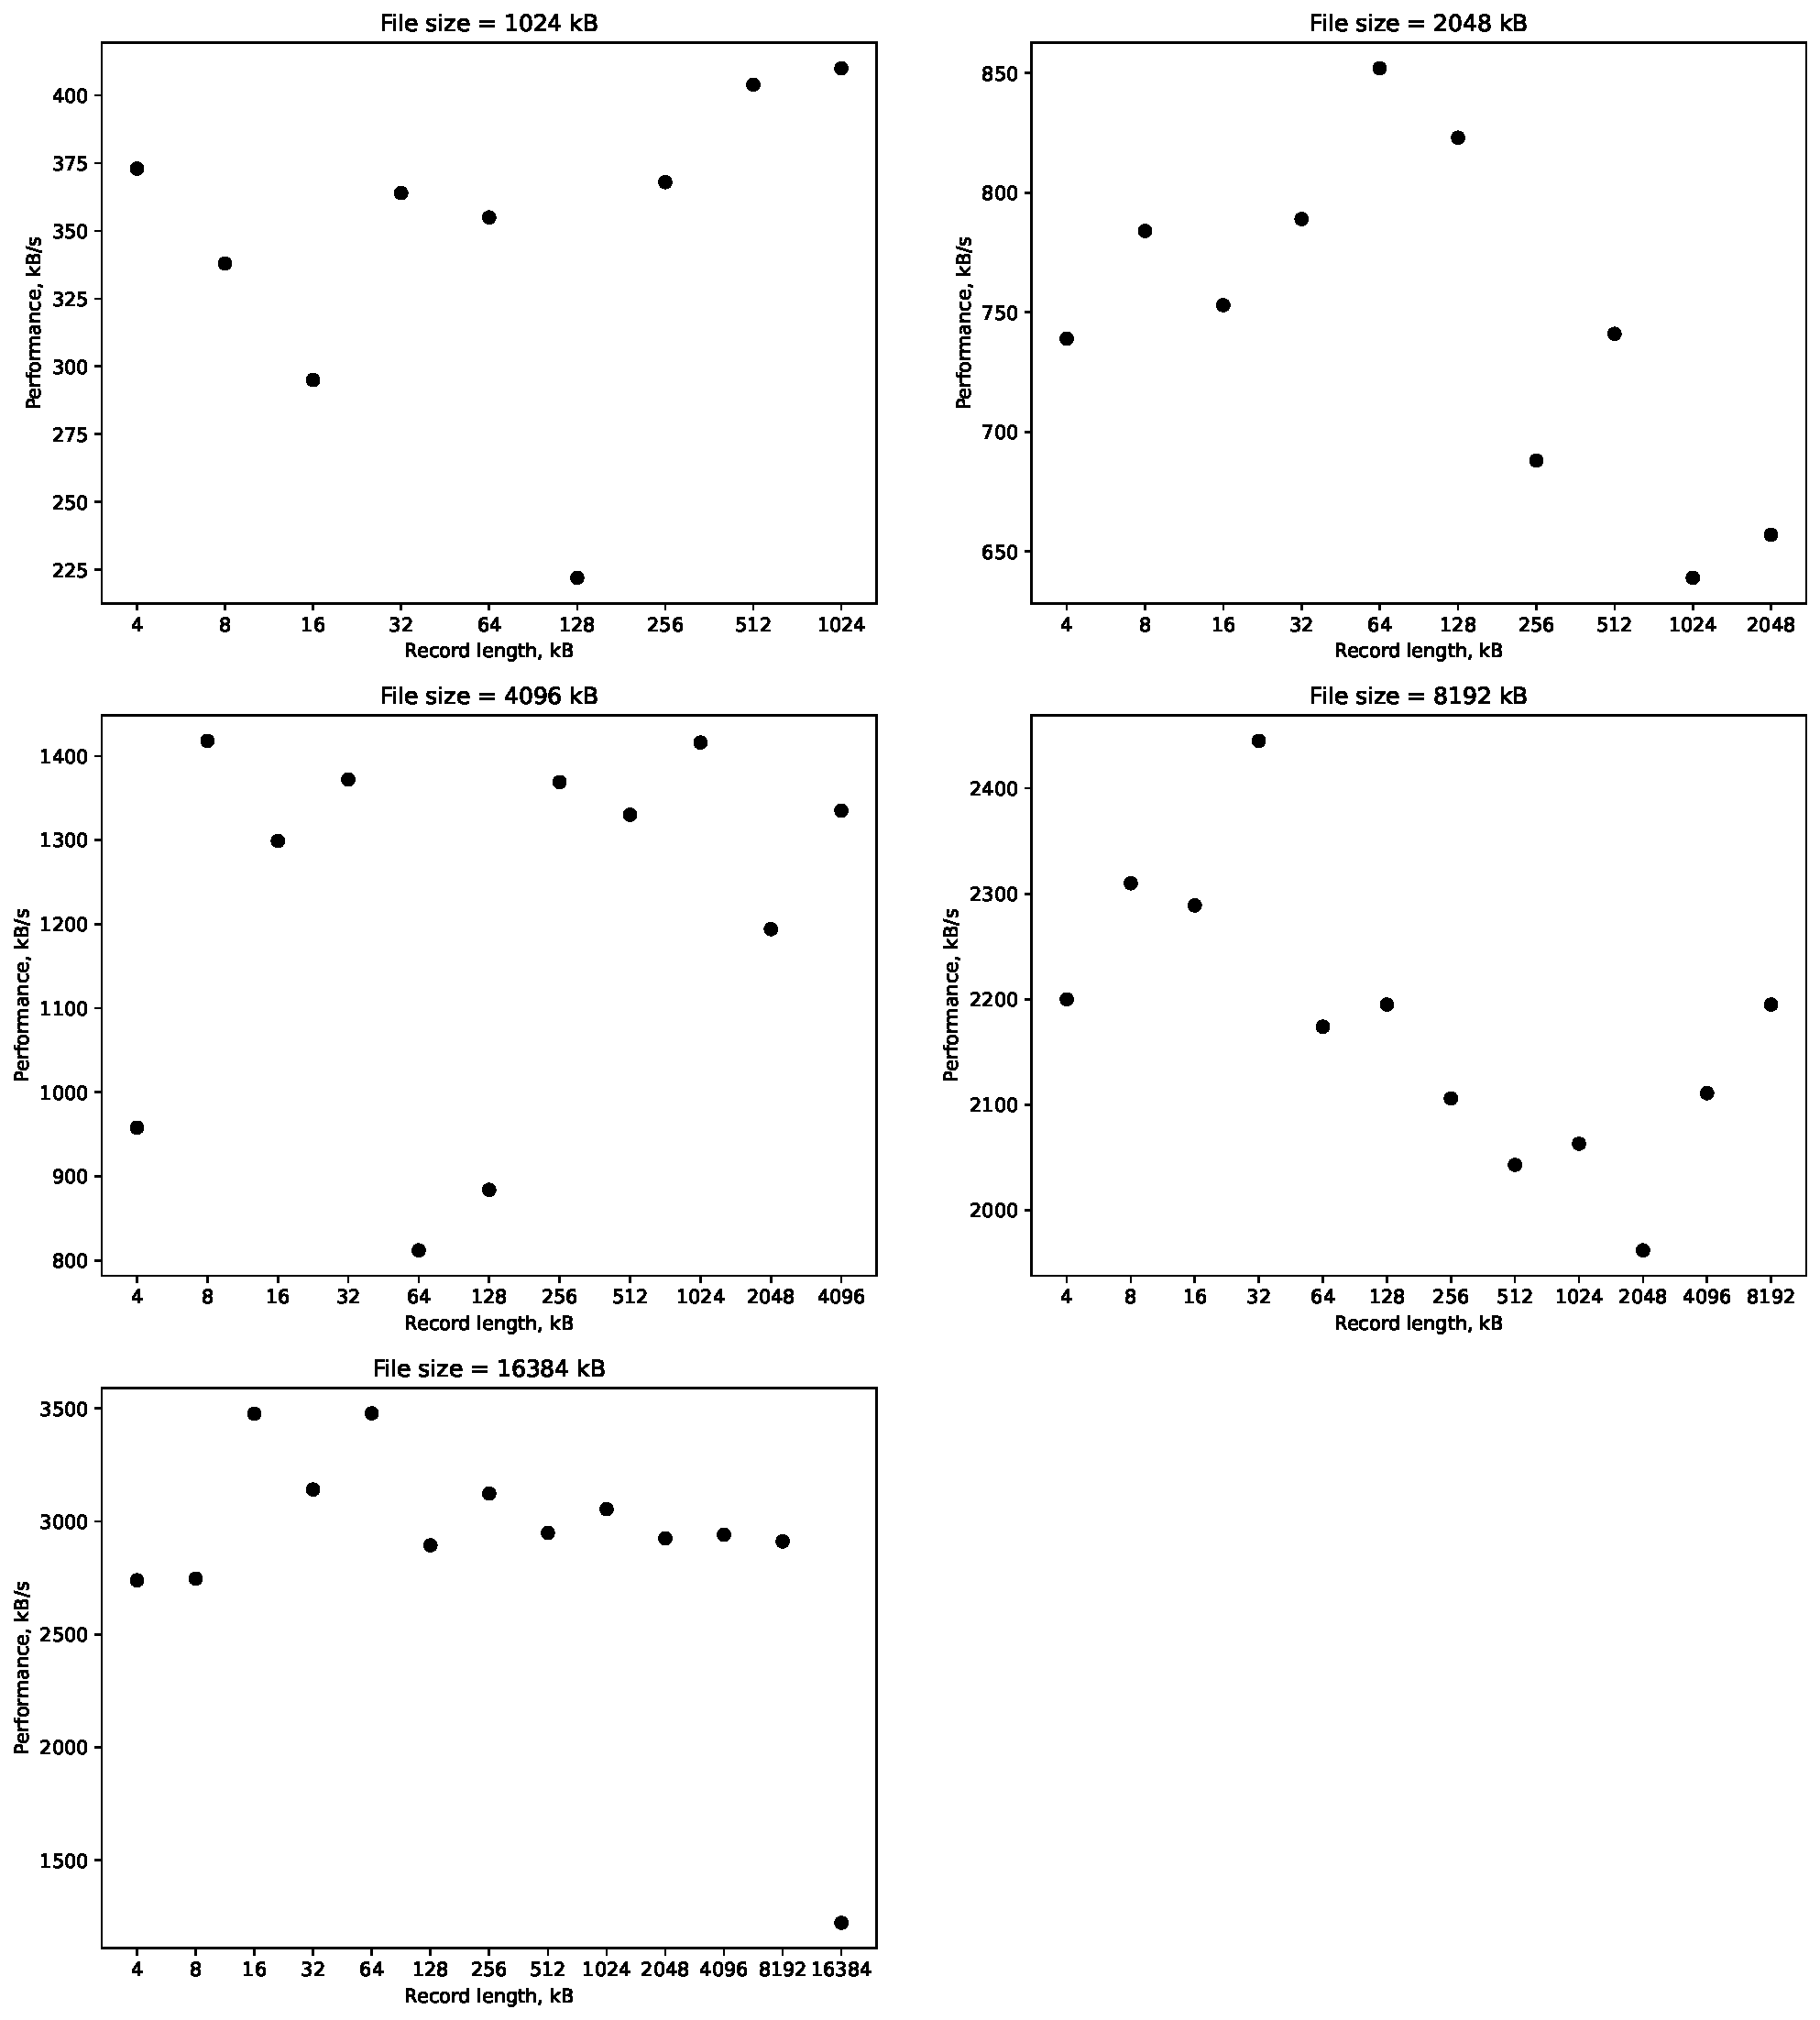
\includegraphics[width=1.0\textwidth]{figures/benchmarking/gcsf/Random write.pdf}
	\end{center}
	\caption{IOZone output for GCSF Random write}
\end{figure}
\section{Fejk FFS}

\begin{table}[!ht]
	\begin{center}
		\caption{IOZone result for Fake FFS Read}
		\resizebox{\textwidth}{!}{\begin{tabular}{| c | c | c | c | c | c | c | c | c | c | c | c | c | c | }
			
			\hline
			{} & \multicolumn{13}{c |}{Buffer size (kB)} \\
			\textbf{File size (kB)}   & 4 & 8 & 16 & 32 & 64 & 128 & 256 & 512 & 1024 & 2048 & 4096 & 8192 & 16384\\
			\hline
			\hline
			\textbf{1024}  & 1992279 & 3314514 & 4114719 & 3791442 & 3241960 & 3239514 & 2008114 & 3160839 & 3291652 & {} & {} & {} & {}\\
			\textbf{2048}  & 2243502 & 2913021 & 4796687 & 5280246 & 3835124 & 5900467 & 5238385 & 4796687 & 3931669 & 4697018 & {} & {} & {}\\
			\textbf{4096}  & 2866270 & 3096138 & 4501111 & 2375927 & 5841891 & 6449370 & 5581856 & 5810280 & 7301864 & 4404184 & 5382492 & {} & {}\\
			\textbf{8192}  & 3010894 & 2750802 & 4196452 & 5665431 & 6616796 & 6838023 & 6410631 & 6211306 & 6643663 & 4571055 & 5765244 & 5553712 & {}\\
			\textbf{16384}  & 3230846 & 3842338 & 4895314 & 5683144 & 6063230 & 6619859 & 6407526 & 7173368 & 6590654 & 6511962 & 6316241 & 5391113 & 5329650\\


			\hline

		\end{tabular}}
		\label{tbl:fs_impl_op}
	\end{center}
\end{table}
	
\begin{table}[!ht]
	\begin{center}
		\caption{IOZone result for Fejk FFS Write}
		\resizebox{\textwidth}{!}{\begin{tabular}{| c | c | c | c | c | c | c | c | c | c | c | c | c | c | }
			
			\hline
			{} & \multicolumn{13}{c |}{Buffer size (kB)} \\
			\textbf{File size (kB)}   & 4 & 8 & 16 & 32 & 64 & 128 & 256 & 512 & 1024 & 2048 & 4096 & 8192 & 16384\\
			\hline
			\hline
			\textbf{1024}  & 6486 & 6595 & 6647 & 6667 & 6558 & 6559 & 85355 & 7342 & 6026 & {} & {} & {} & {}\\
			\textbf{2048}  & 6499 & 6807 & 7030 & 7035 & 7233 & 116330 & 7192 & 6963 & 109349 & 7212 & {} & {} & {}\\
			\textbf{4096}  & 6614 & 7140 & 7266 & 6590 & 7044 & 7187 & 7103 & 7250 & 7226 & 6897 & 6983 & {} & {}\\
			\textbf{8192}  & 4833 & 5677 & 6189 & 7044 & 6998 & 7219 & 7231 & 7167 & 110695 & 113346 & 7182 & 7269 & {}\\
			\textbf{16384}  & 7163 & 7174 & 7479 & 7516 & 7569 & 7787 & 7473 & 7774 & 7688 & 7628 & 7438 & 7294 & 7503\\


			\hline

		\end{tabular}}
		\label{tbl:data_write_fejk_ffs}
	\end{center}
\end{table}
	
\begin{table}[!ht]
	\begin{center}
		\caption{IOZone result for Fake FFS Re-Read}
		\resizebox{\textwidth}{!}{\begin{tabular}{| c | c | c | c | c | c | c | c | c | c | c | c | c | c | }
			
			\hline
			{} & \multicolumn{13}{c |}{Buffer size (kB)} \\
			\textbf{File size (kB)}   & 4 & 8 & 16 & 32 & 64 & 128 & 256 & 512 & 1024 & 2048 & 4096 & 8192 & 16384\\
			\hline
			\hline
			\textbf{1024}  & 2197132 & 4029784 & 4574926 & 5652717 & 5417427 & 4493556 & 5120336 & 3941039 & 4594502 & {} & {} & {} & {}\\
			\textbf{2048}  & 3024831 & 2994254 & 4911886 & 5765808 & 4741090 & 7059413 & 5020987 & 5184636 & 4886737 & 6629029 & {} & {} & {}\\
			\textbf{4096}  & 3122019 & 3540193 & 5468151 & 4376138 & 7038605 & 7925004 & 6659365 & 6321227 & 7715028 & 5490871 & 5291314 & {} & {}\\
			\textbf{8192}  & 2886449 & 2338541 & 4554091 & 6249718 & 5940679 & 7793434 & 7236972 & 8062248 & 6272536 & 7281448 & 5465373 & 5509188 & {}\\
			\textbf{16384}  & 3351874 & 3992114 & 5232657 & 6129753 & 7356911 & 7861915 & 7123547 & 8388806 & 7180114 & 6907309 & 6511962 & 4982992 & 5403831\\


			\hline

		\end{tabular}}
		\label{tbl:fs_impl_op}
	\end{center}
\end{table}
	
\begin{table}[!ht]
	\begin{center}
		\caption{IOZone result for Fake FFS Re-Write}
		\resizebox{\textwidth}{!}{\begin{tabular}{| c | c | c | c | c | c | c | c | c | c | c | c | c | c | }
			
			\hline
			{} & \multicolumn{13}{c |}{Buffer size (kB)} \\
			\textbf{File size (kB)}   & 4 & 8 & 16 & 32 & 64 & 128 & 256 & 512 & 1024 & 2048 & 4096 & 8192 & 16384\\
			\hline
			\hline
			\textbf{1024}  & 4860 & 6161 & 6096 & 5938 & 6321 & 6364 & 6297 & 5894 & 6383 & {} & {} & {} & {}\\
			\textbf{2048}  & 5942 & 6061 & 6376 & 6386 & 6418 & 6268 & 6373 & 34391 & 37349 & 6452 & {} & {} & {}\\
			\textbf{4096}  & 6084 & 6174 & 6233 & 6413 & 6370 & 6415 & 6422 & 6143 & 6434 & 6392 & 6433 & {} & {}\\
			\textbf{8192}  & 4744 & 5055 & 5045 & 5912 & 5832 & 5625 & 5764 & 5798 & 5917 & 25475 & 5799 & 5912 & {}\\
			\textbf{16384}  & 6109 & 6150 & 5047 & 6336 & 6474 & 6574 & 6391 & 6498 & 6381 & 5934 & 6154 & 6245 & 6322\\


			\hline

		\end{tabular}}
		\label{tbl:data_re-write_fake_ffs}
	\end{center}
\end{table}
	
\begin{table}[!ht]
	\begin{center}
		\caption{IOZone result for Fake FFS Random read}
		\resizebox{\textwidth}{!}{\begin{tabular}{| c | c | c | c | c | c | c | c | c | c | c | c | c | c | }
			
			\hline
			{} & \multicolumn{13}{c |}{Buffer size (kB)} \\
			\textbf{File size (kB)}   & 4 & 8 & 16 & 32 & 64 & 128 & 256 & 512 & 1024 & 2048 & 4096 & 8192 & 16384\\
			\hline
			\hline
			\textbf{1024}  & 1549519 & 3085895 & 4805258 & 5751117 & 4232305 & 6569179 & 5630486 & 4805258 & 5564829 & {} & {} & {} & {}\\
			\textbf{2048}  & 2455806 & 3020577 & 5593112 & 7237860 & 5251194 & 8261095 & 6024617 & 4829046 & 2348384 & 6479029 & {} & {} & {}\\
			\textbf{4096}  & 2299908 & 3129412 & 4853336 & 3834958 & 7286380 & 8625273 & 7367624 & 7197849 & 7225093 & 5565581 & 5944991 & {} & {}\\
			\textbf{8192}  & 2271747 & 2173593 & 4003788 & 5599873 & 6720329 & 7340560 & 7261443 & 8030217 & 6191160 & 5504775 & 5979968 & 5872650 & {}\\
			\textbf{16384}  & 2310146 & 2878929 & 4302549 & 5402132 & 7053355 & 6860418 & 7005182 & 7533538 & 6318564 & 7040348 & 6878271 & 5483167 & 5457909\\


			\hline

		\end{tabular}}
		\label{tbl:fs_impl_op}
	\end{center}
\end{table}
	
\begin{table}[!ht]
	\begin{center}
		\caption{IOZone result for Fake FFS Random write}
		\resizebox{\textwidth}{!}{\begin{tabular}{| c | c | c | c | c | c | c | c | c | c | c | c | c | c | }
			
			\hline
			{} & \multicolumn{13}{c |}{Buffer size (kB)} \\
			\textbf{File size (kB)}   & 4 & 8 & 16 & 32 & 64 & 128 & 256 & 512 & 1024 & 2048 & 4096 & 8192 & 16384\\
			\hline
			\hline
			\textbf{1024}  & 5864 & 6137 & 6251 & 6146 & 6362 & 6252 & 5775 & 6457 & 6352 & {} & {} & {} & {}\\
			\textbf{2048}  & 5869 & 6190 & 6252 & 6124 & 6398 & 6533 & 6415 & 6331 & 6587 & 6546 & {} & {} & {}\\
			\textbf{4096}  & 5871 & 6067 & 6273 & 6436 & 6521 & 6467 & 6325 & 6507 & 6495 & 6433 & 6474 & {} & {}\\
			\textbf{8192}  & 4923 & 4113 & 4917 & 5871 & 5843 & 5937 & 5954 & 5965 & 5961 & 5907 & 5954 & 6169 & {}\\
			\textbf{16384}  & 6151 & 6081 & 5323 & 6342 & 6399 & 6219 & 6462 & 6278 & 6355 & 5947 & 5092 & 6248 & 6404\\


			\hline

		\end{tabular}}
		\label{tbl:data_random_write_fake_ffs}
	\end{center}
\end{table}
	

\begin{figure}[!htb]
	\label{fig:app_bencfh_ffs_read}
	\begin{center}
		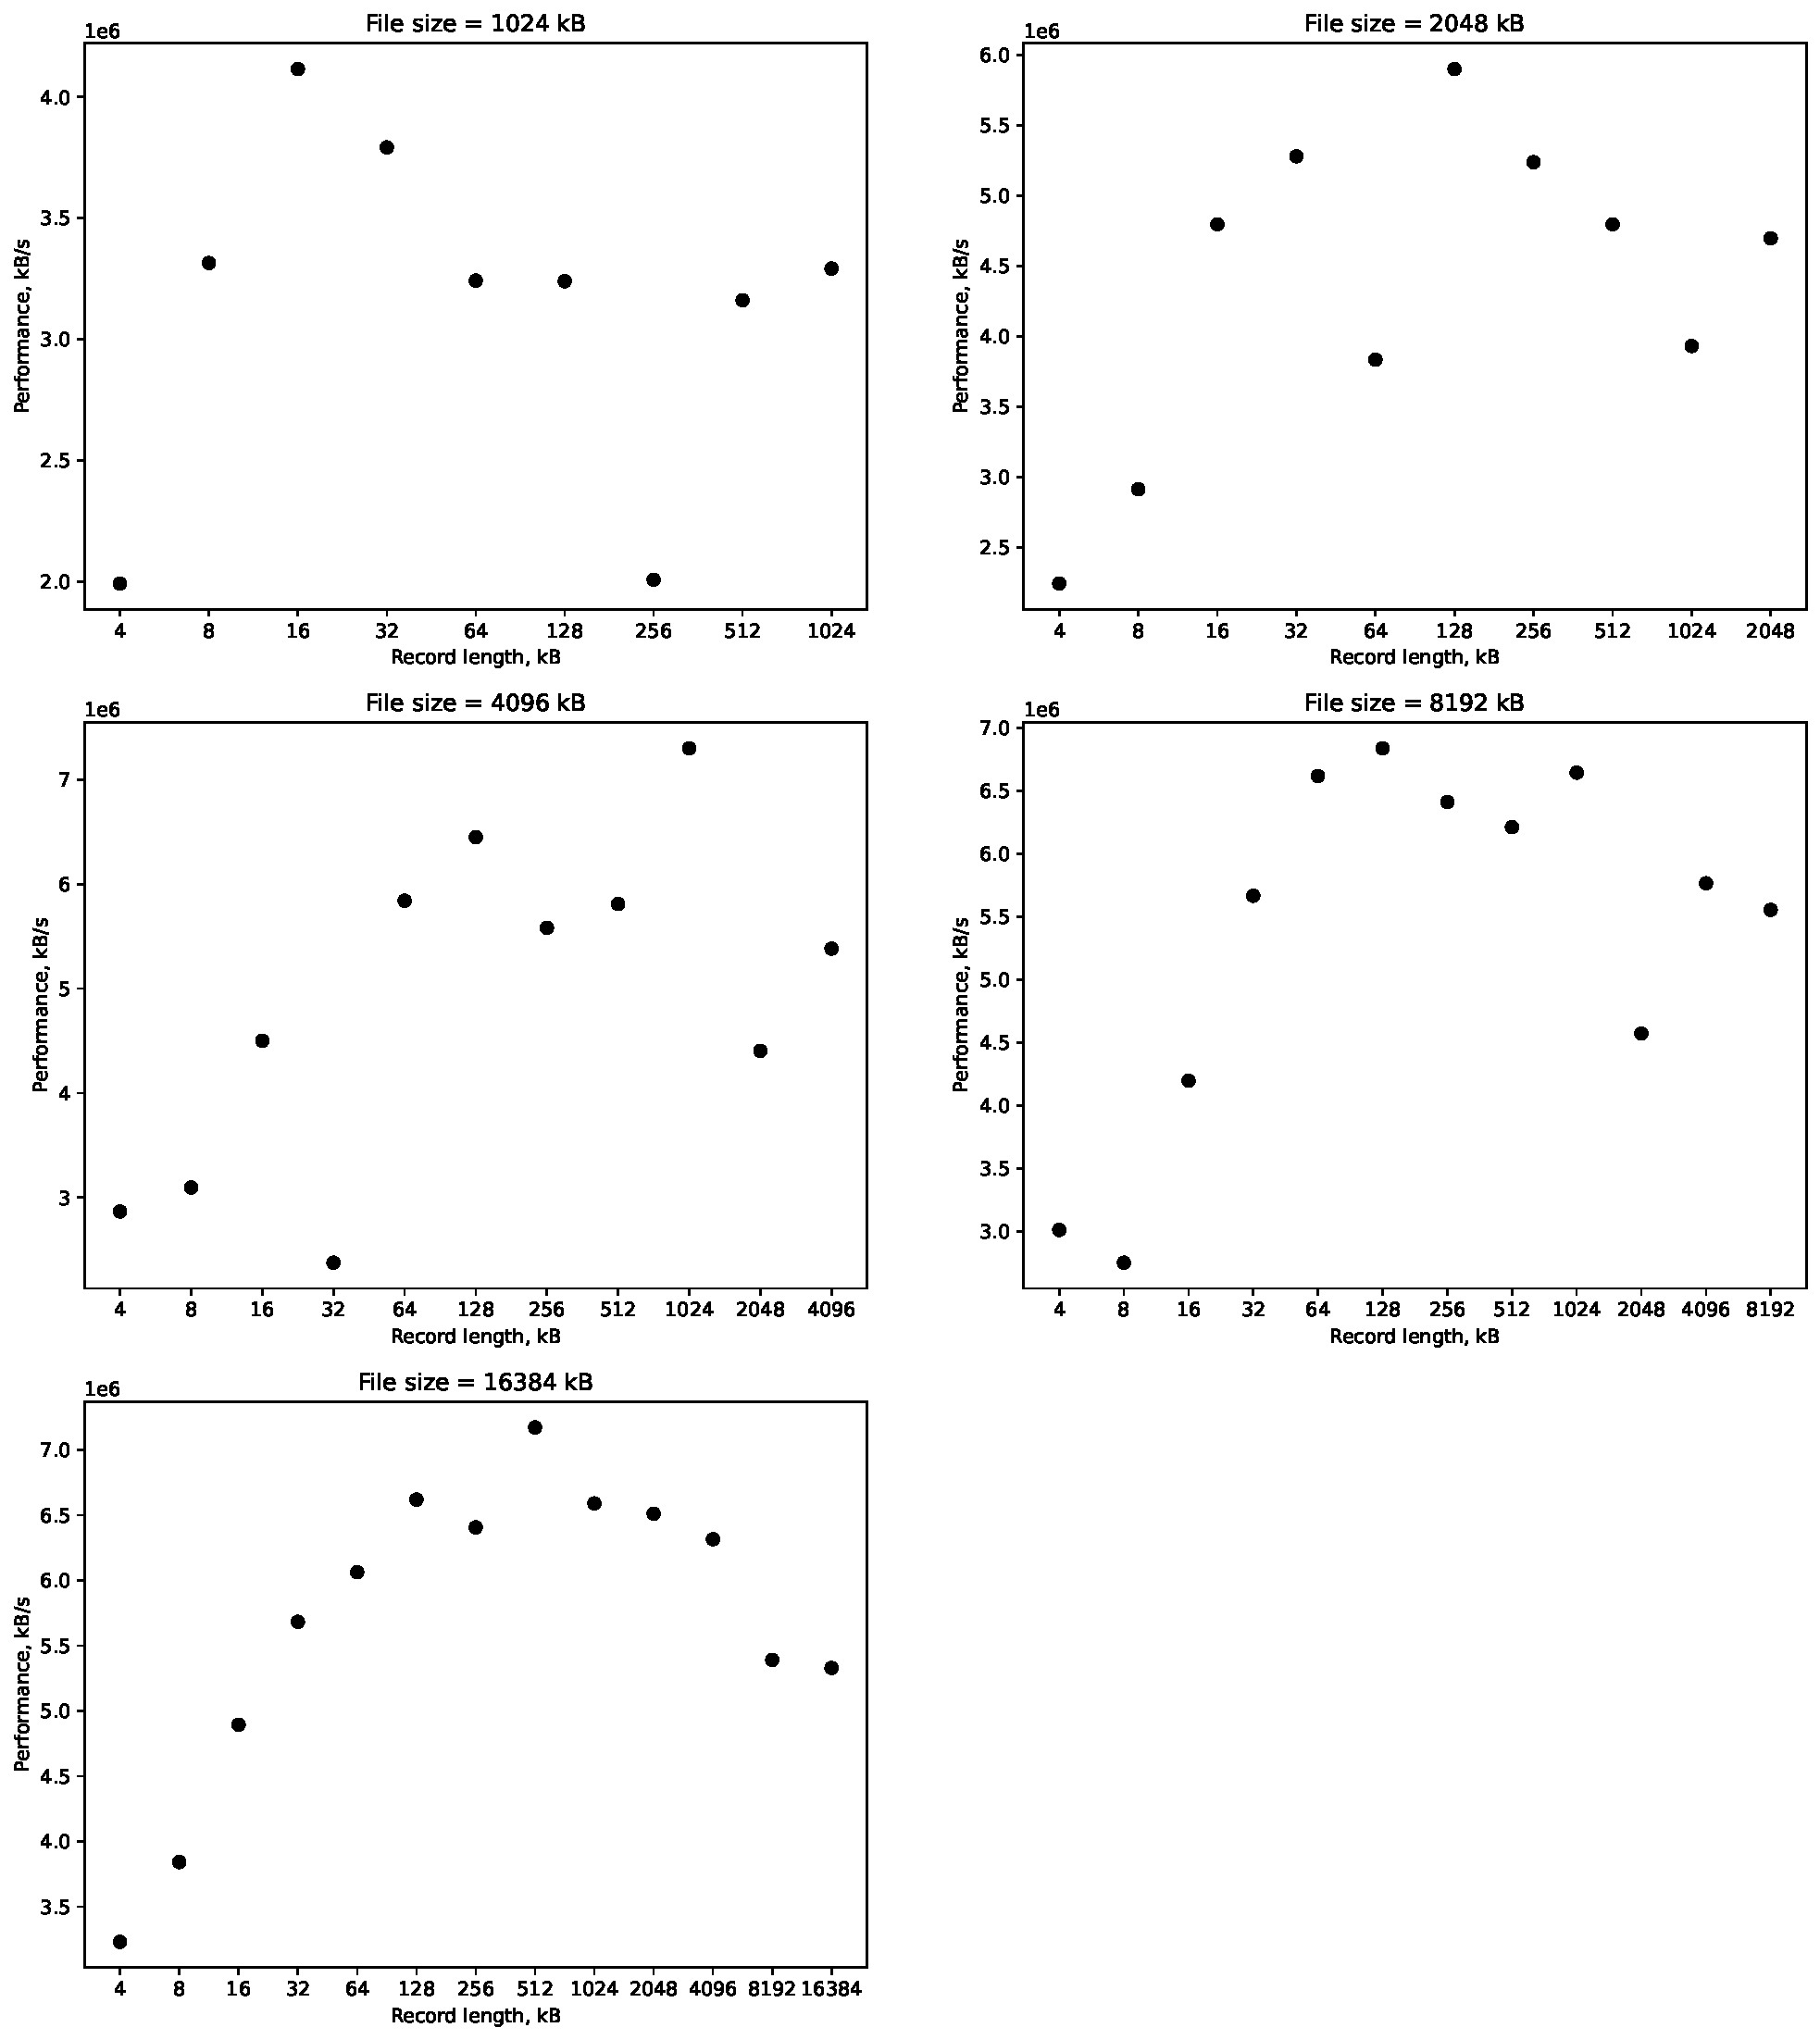
\includegraphics[width=1.0\textwidth]{figures/benchmarking/fake-ffs/Read.pdf}
	\end{center}
	\caption{IOZone output for Fejk FFS Forward Read}
\end{figure}

\begin{figure}[!htb]
	\label{fig:app_benchf_ffs_write}
	\begin{center}
		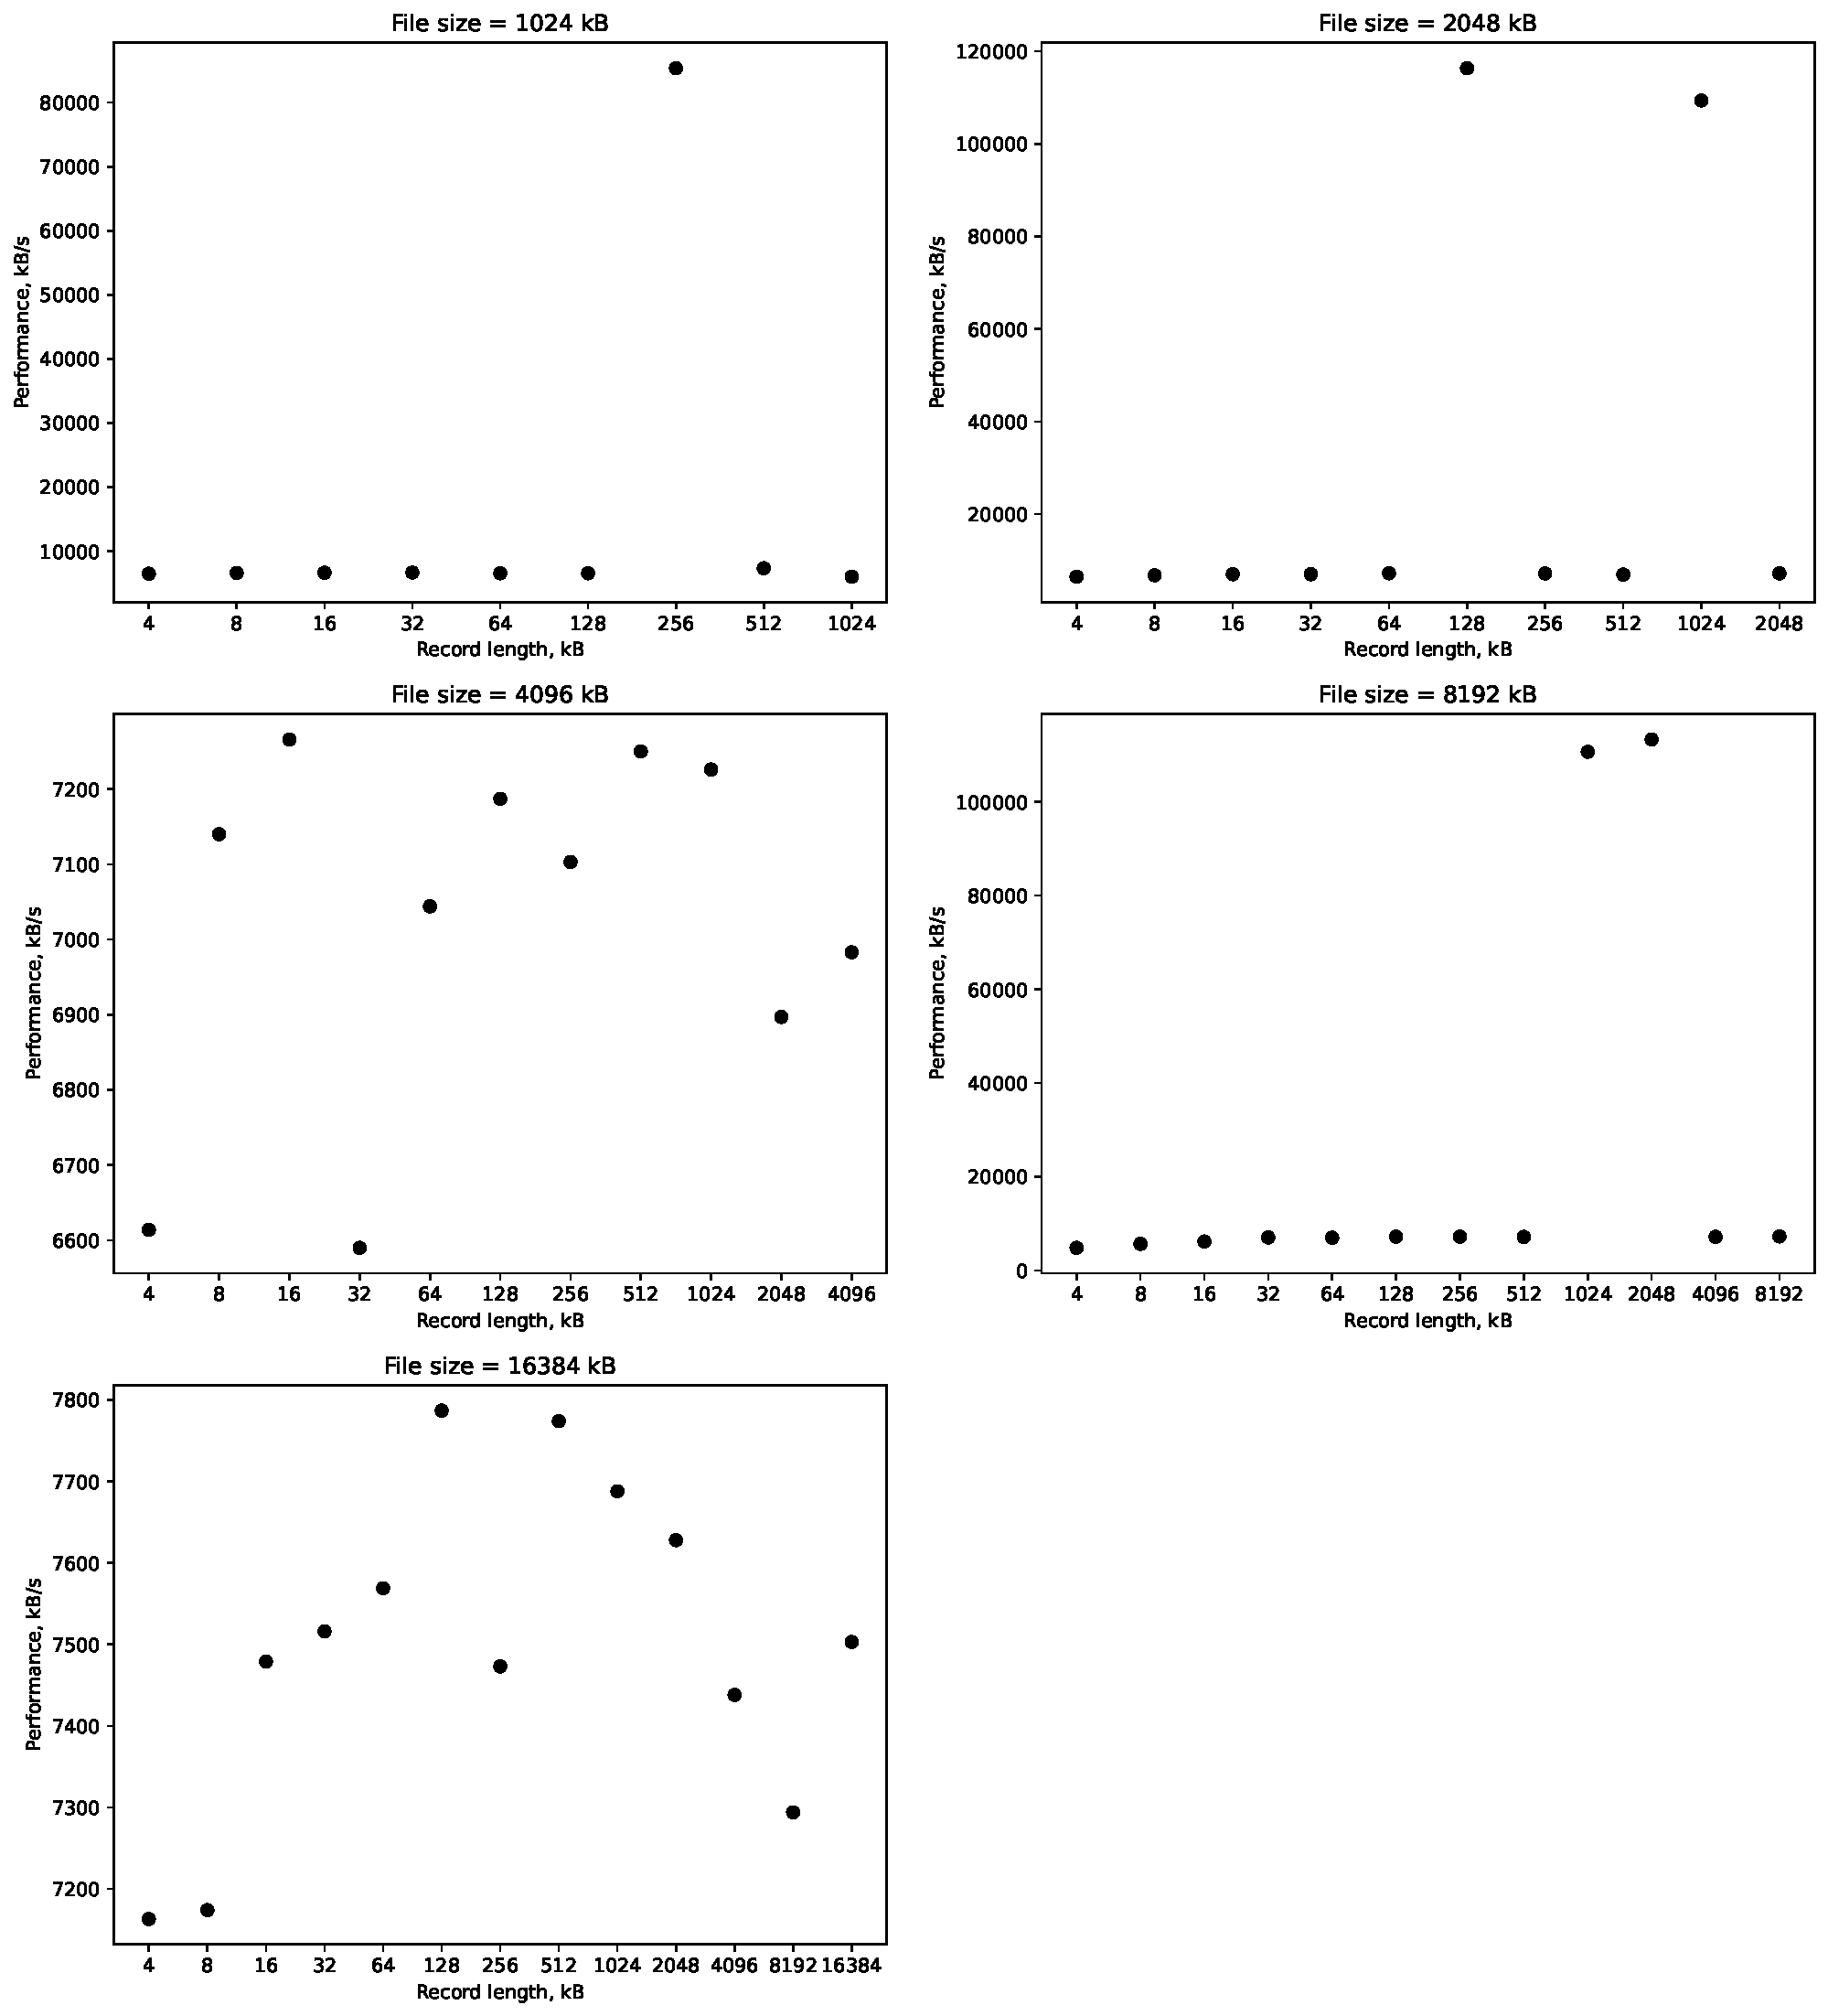
\includegraphics[width=1.0\textwidth]{figures/benchmarking/fake-ffs/Write.pdf}
	\end{center}
	\caption{IOZone output for Fejk FFS Forward Write}
\end{figure}

\begin{figure}[!htb]
	\label{fig:app_bench_fffs_re_read}
	\begin{center}
		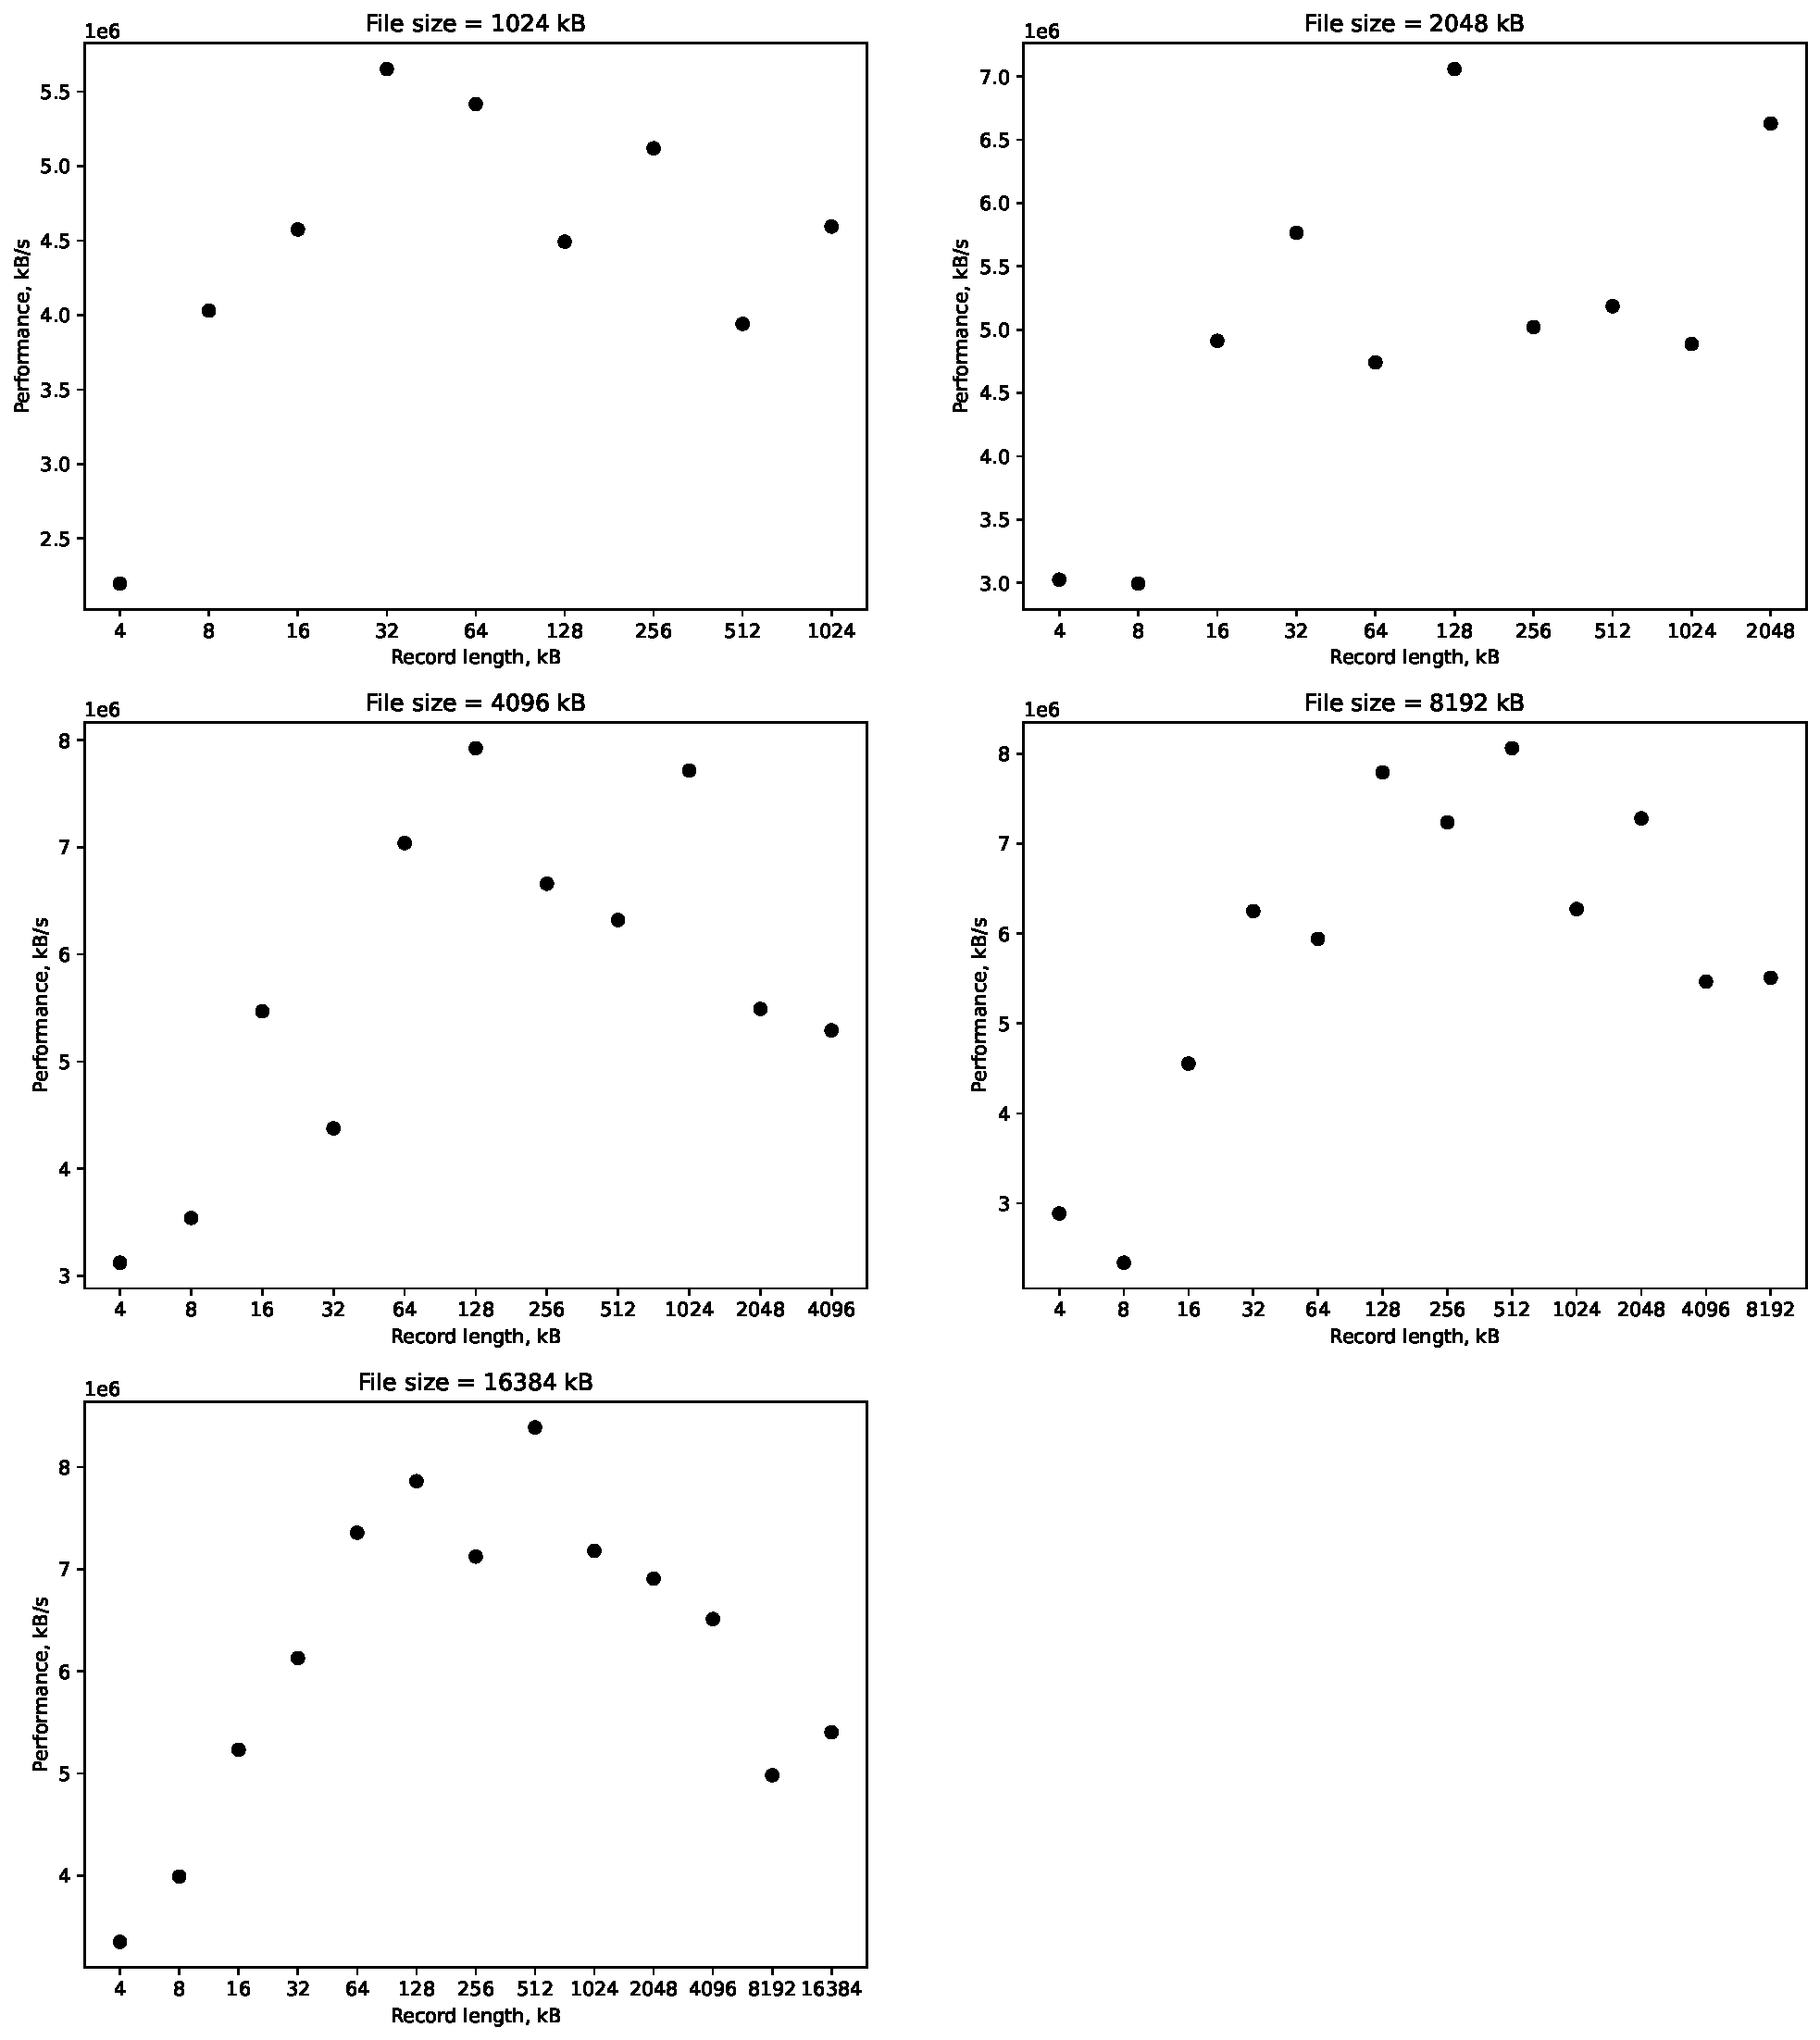
\includegraphics[width=1.0\textwidth]{figures/benchmarking/fake-ffs/Re-Read.pdf}
	\end{center}
	\caption{IOZone output for Fejk FFS Re-Read}
\end{figure}

\begin{figure}[!htb]
	\label{fig:app_bench_fffs_re_write}
	\begin{center}
		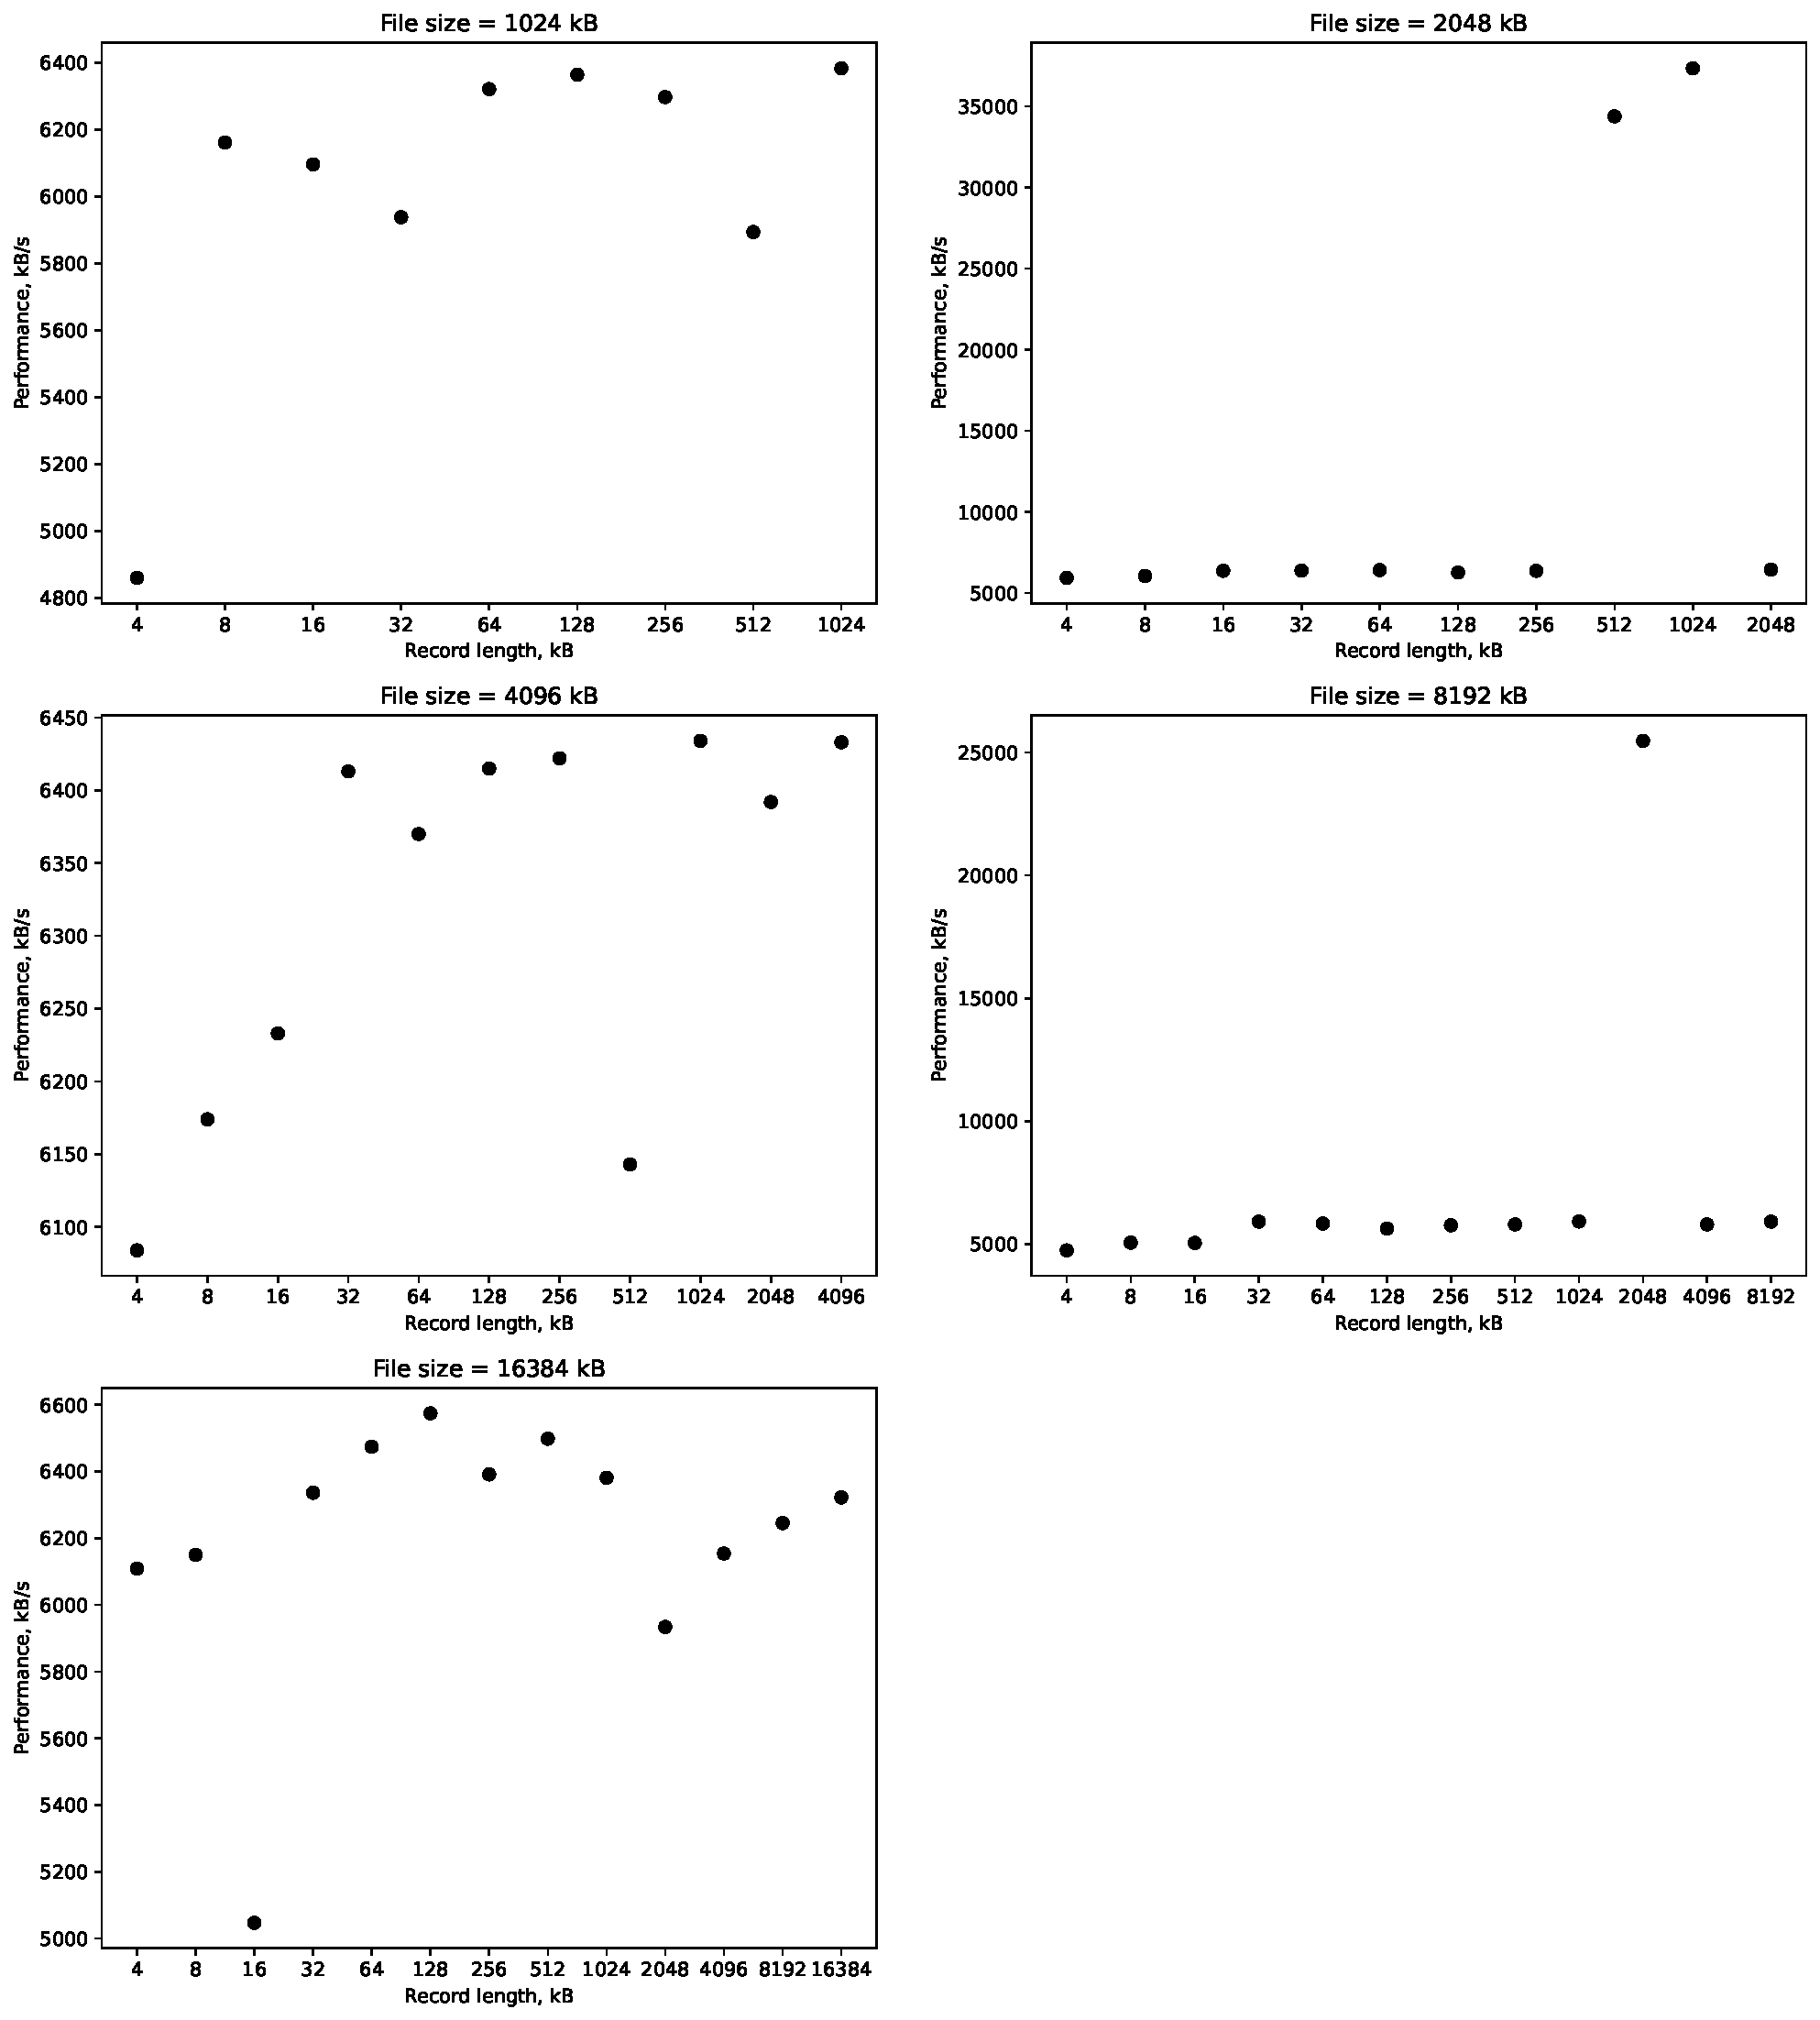
\includegraphics[width=1.0\textwidth]{figures/benchmarking/fake-ffs/Re-Write.pdf}
	\end{center}
	\caption{IOZone output for Fejk FFS Re-Write}
\end{figure}

\begin{figure}[!htb]
	\label{fig:app_bench_fffs_rnd_read}
	\begin{center}
		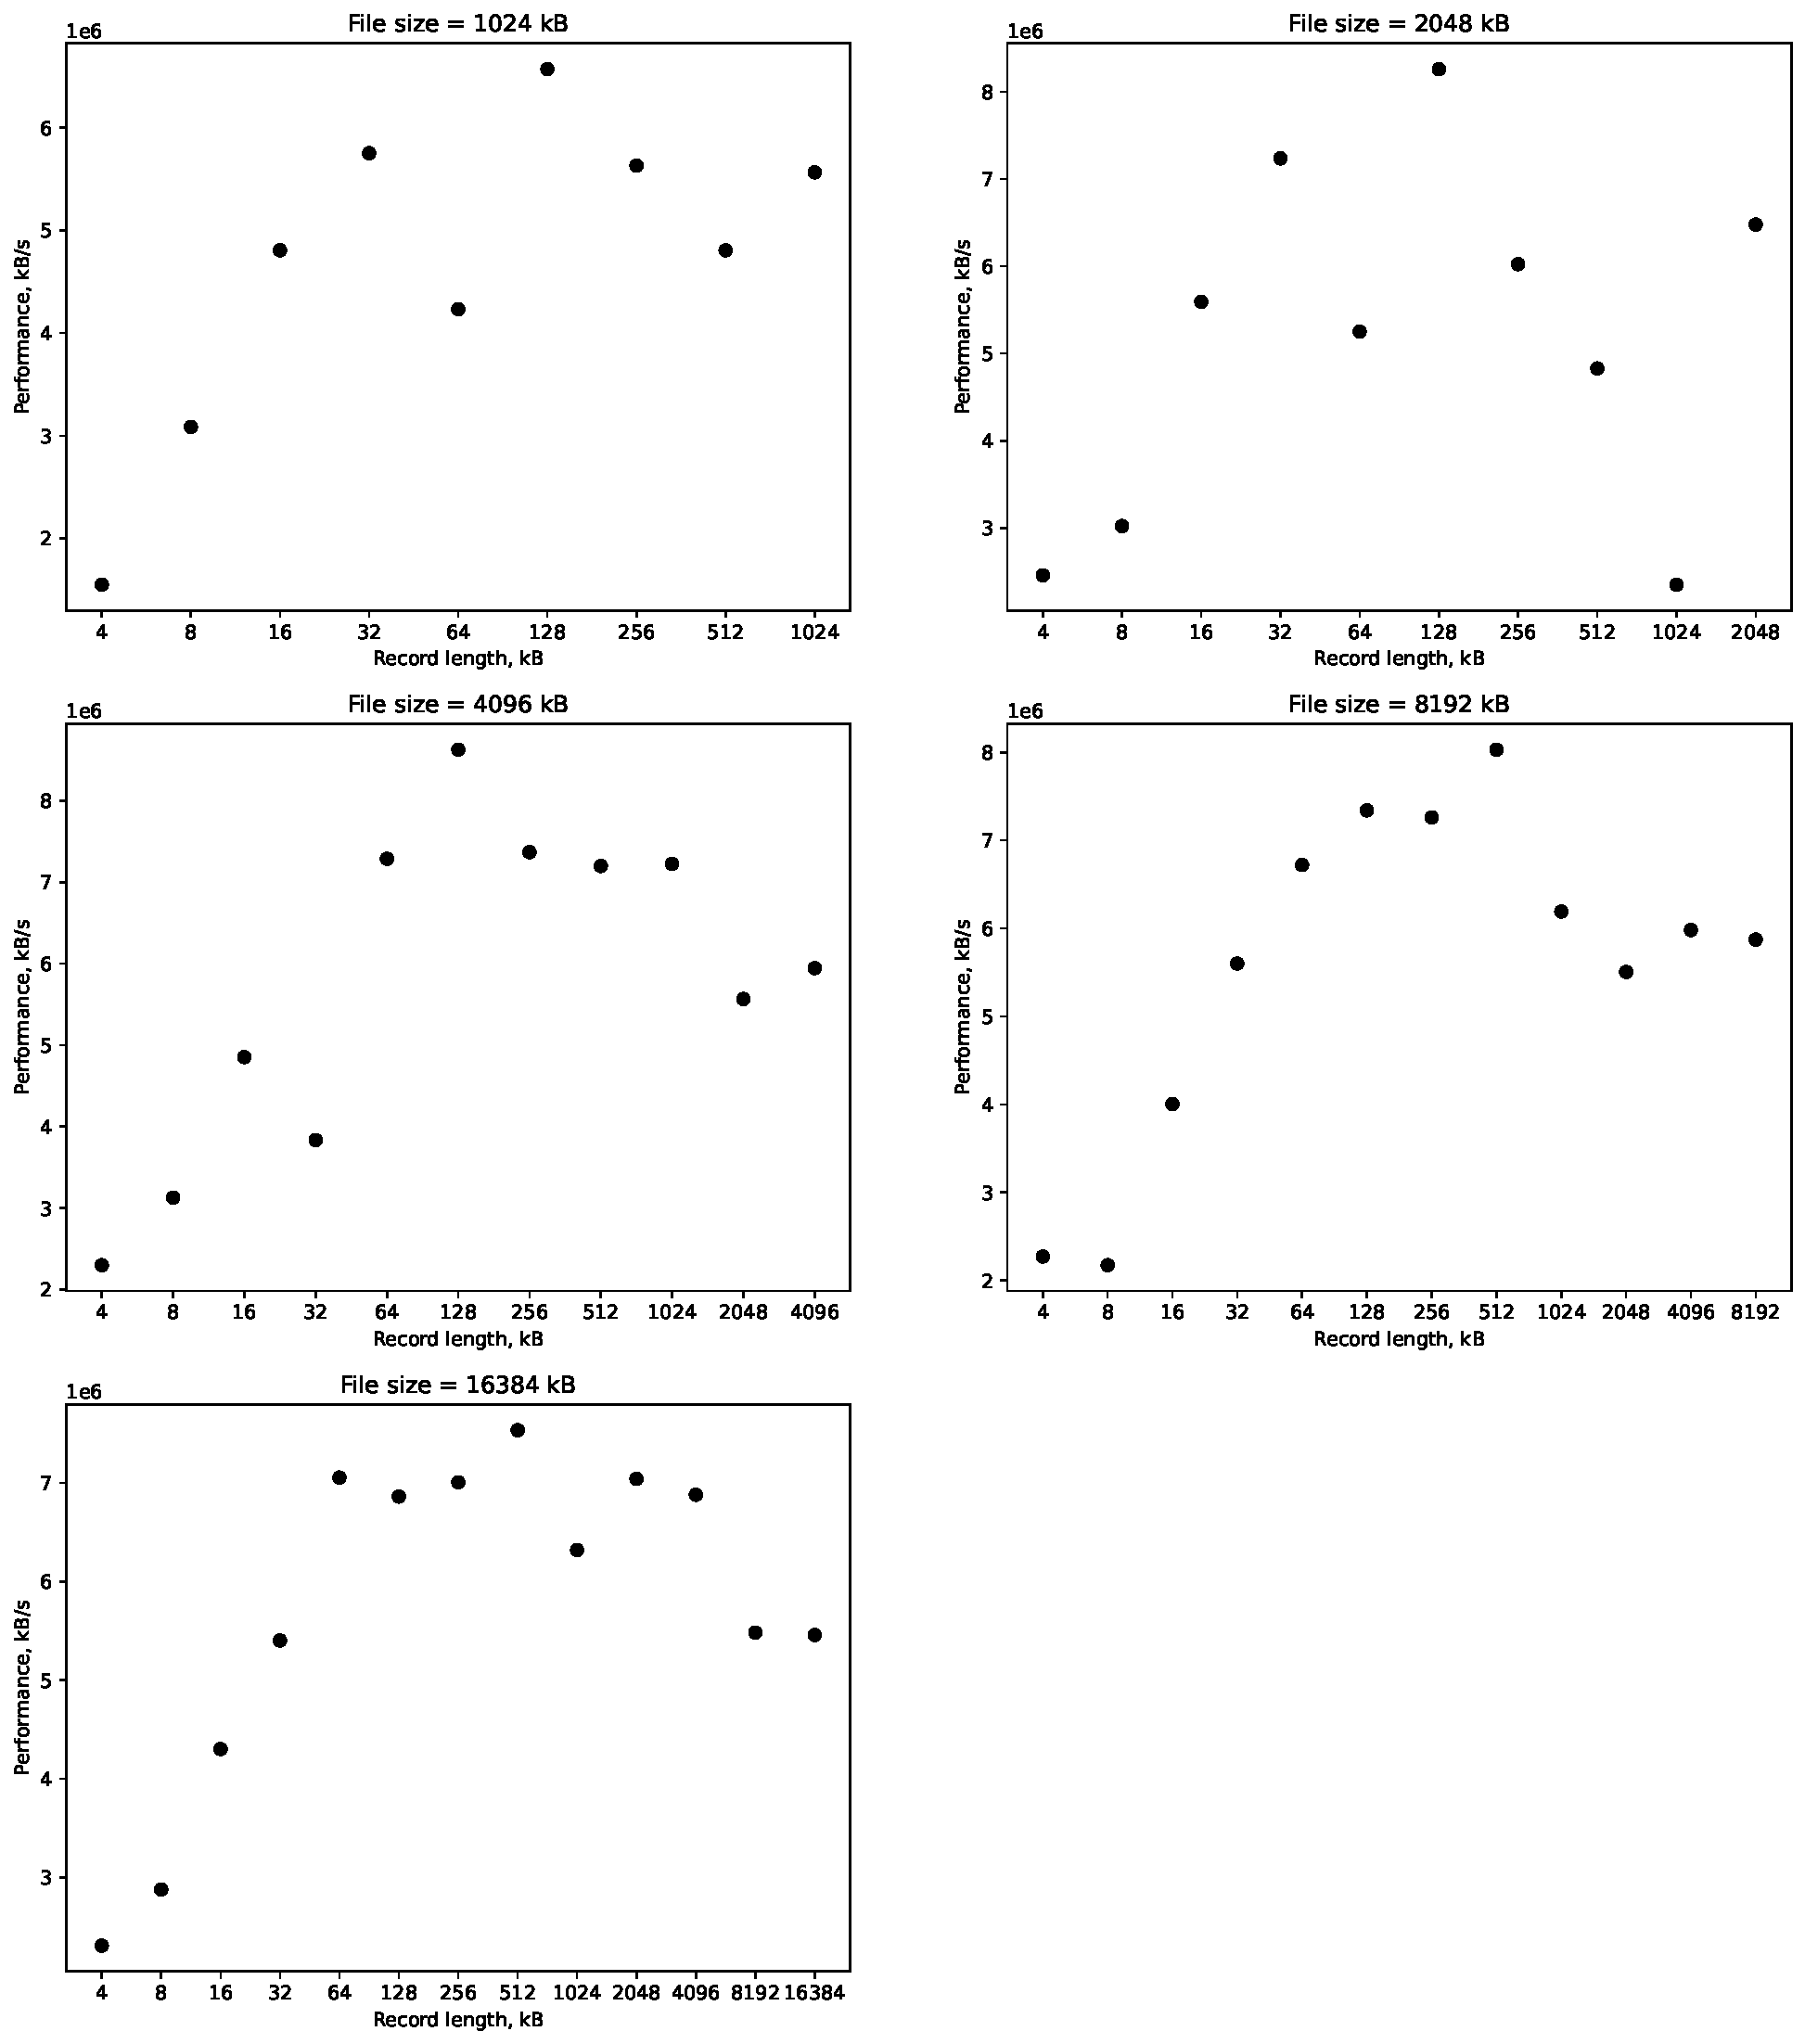
\includegraphics[width=1.0\textwidth]{figures/benchmarking/fake-ffs/Random read.pdf}
	\end{center}
	\caption{IOZone output for Fejk FFS Random read}
\end{figure}

\begin{figure}[!htb]
	\label{fig:app_bench_ffsf_rnd_write}
	\begin{center}
		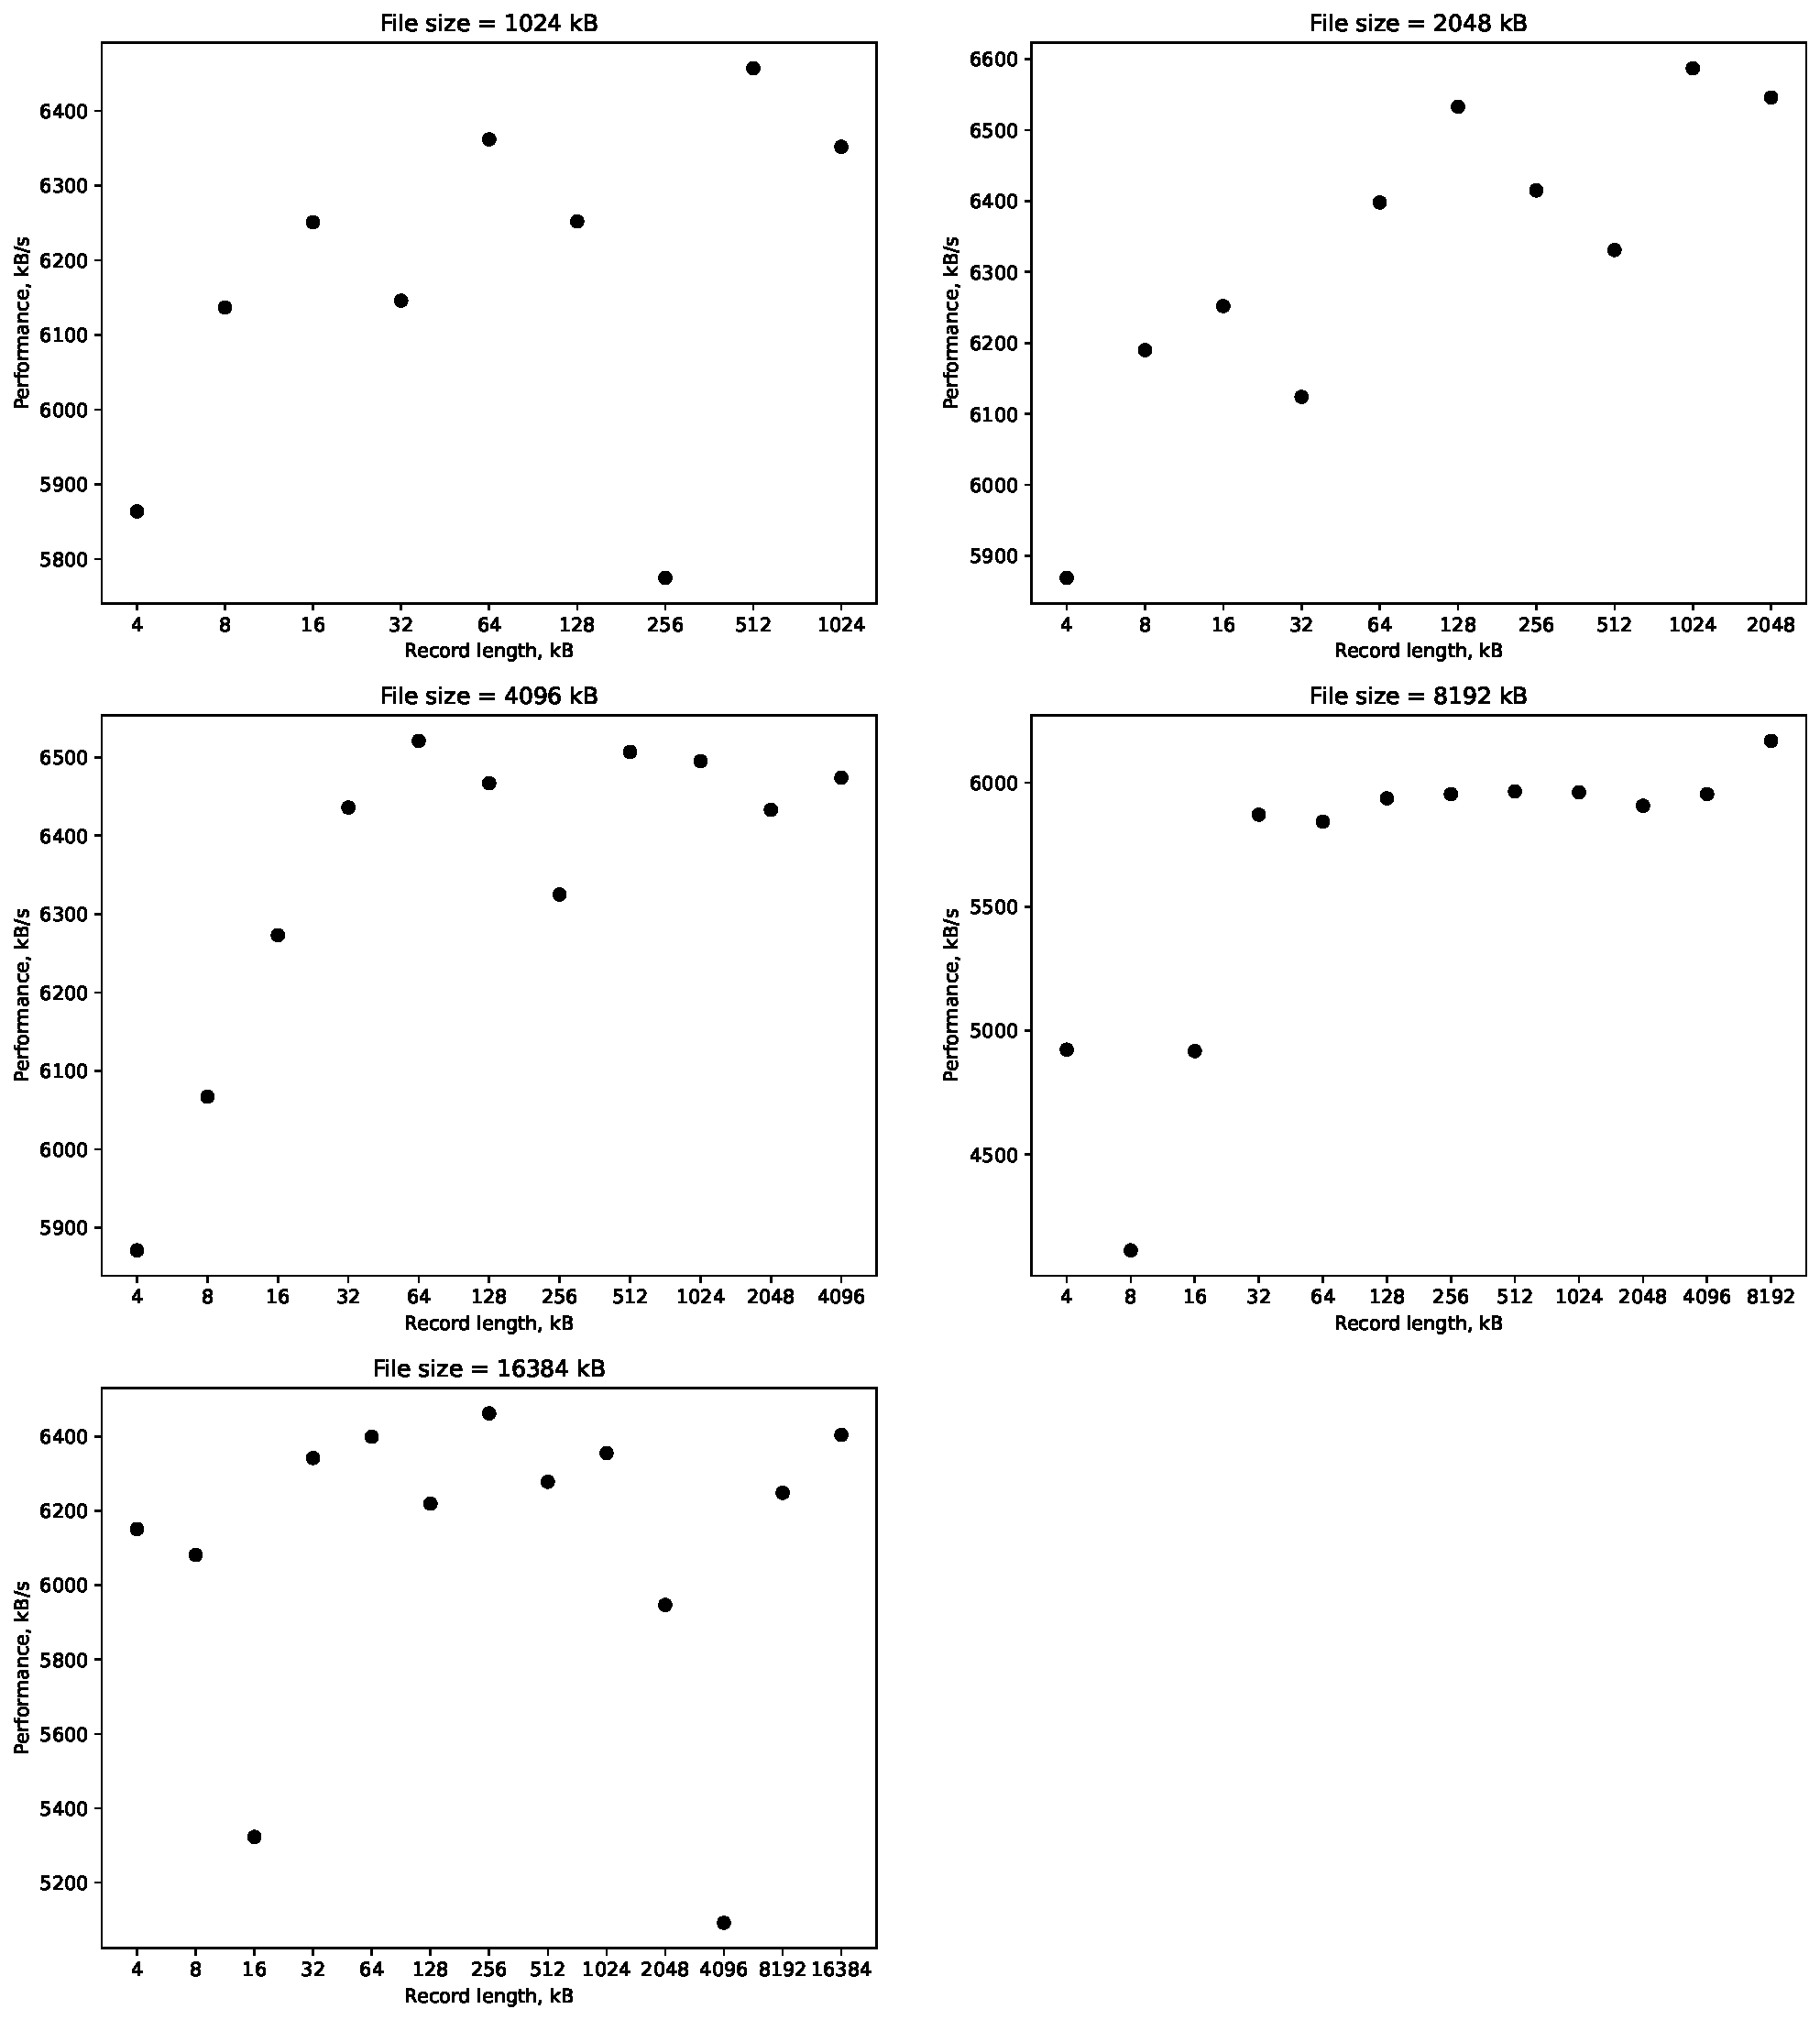
\includegraphics[width=1.0\textwidth]{figures/benchmarking/fake-ffs/Random write.pdf}
	\end{center}
	\caption{IOZone output for Fejk FFS Random write}
\end{figure}
\section{APFS}

\begin{table}[!ht]
	\begin{center}
		\caption{IOZone result for the Read test on APFS}
		\resizebox{\textwidth}{!}{\begin{tabular}{| c | c | c | c | c | c | c | c | c | c | c | c | c | c | }
			
			\hline
			{} & \multicolumn{13}{c |}{Buffer size (kB)} \\
			\textbf{File size (kB)}   & 4 & 8 & 16 & 32 & 64 & 128 & 256 & 512 & 1024 & 2048 & 4096 & 8192 & 16384\\
			\hline
			\hline
			\textbf{1024}  & 2300703 & 3472628 & 5444898 & 6025439 & 3425544 & 2353657 & 3521025 & 5479632 & 1259592 & {} & {} & {} & {}\\
			\textbf{2048}  & 2429413 & 3548378 & 2324238 & 2288326 & 2392202 & 7817519 & 5277002 & 6939647 & 6867521 & 7529708 & {} & {} & {}\\
			\textbf{4096}  & 2597576 & 3931494 & 4922872 & 3456849 & 6151473 & 6908408 & 7064655 & 5894001 & 4648477 & 5402804 & 6281934 & {} & {}\\
			\textbf{8192}  & 2693866 & 3716653 & 4555903 & 5487193 & 4143818 & 6405850 & 8054689 & 7585256 & 5708730 & 7537004 & 4594281 & 5576245 & {}\\
			\textbf{16384}  & 1887130 & 3339494 & 5330063 & 3537899 & 6635840 & 6409917 & 6430310 & 4554938 & 6921222 & 3453620 & 2166589 & 5158807 & 4187197\\
			\textbf{32768}  & 2452479 & 2775321 & 4702013 & 6173478 & 5991547 & 6411354 & 6621073 & 5601338 & 7129387 & 6994417 & 5692749 & 5448563 & 4751758\\
			\textbf{65536}  & 2673966 & 4183591 & 5032015 & 6032415 & 6770924 & 6720270 & 6932816 & 7149936 & 6714032 & 6609102 & 6538515 & 5680492 & 5542138\\
			\textbf{131072}  & 2775537 & 4124081 & 5119016 & 5613831 & 5348765 & 6775497 & 4877838 & 5514443 & 4523778 & 5408171 & 2241853 & 2555460 & 2956665\\
			\textbf{262144}  & 2612033 & 4088592 & 5074689 & 6218999 & 6861877 & 6715279 & 6735808 & 7042156 & 6728553 & 3955521 & 5947137 & 4522621 & 5227609\\


			\hline

		\end{tabular}}
		\label{tbl:data_local_read}
	\end{center}
\end{table}
	
\begin{table}[!ht]
	\begin{center}
		\caption{IOZone result for APFS Write}
		\resizebox{\textwidth}{!}{\begin{tabular}{| c | c | c | c | c | c | c | c | c | c | c | c | c | c | }
			
			\hline
			{} & \multicolumn{13}{c |}{Buffer size (kB)} \\
			\textbf{File size (kB)}   & 4 & 8 & 16 & 32 & 64 & 128 & 256 & 512 & 1024 & 2048 & 4096 & 8192 & 16384\\
			\hline
			\hline
			\textbf{1024}  & 157562 & 280097 & 419520 & 220777 & 271116 & 1091532 & 854752 & 1687075 & 305782 & {} & {} & {} & {}\\
			\textbf{2048}  & 180154 & 251044 & 414476 & 397980 & 425248 & 664300 & 379685 & 1344739 & 1421279 & 2102899 & {} & {} & {}\\
			\textbf{4096}  & 186197 & 340567 & 351651 & 934714 & 486051 & 1136174 & 771788 & 1353618 & 784547 & 735918 & 1231902 & {} & {}\\
			\textbf{8192}  & 200062 & 251335 & 403762 & 604799 & 537746 & 1224736 & 745948 & 1595914 & 1381695 & 1063479 & 1439766 & 445727 & {}\\
			\textbf{16384}  & 207663 & 216404 & 111071 & 574597 & 729051 & 1050647 & 941932 & 630420 & 1114024 & 1460506 & 1495696 & 1490829 & 1539559\\


			\hline

		\end{tabular}}
		\label{tbl:fs_impl_op}
	\end{center}
\end{table}
	
\begin{table}[!ht]
	\begin{center}
		\caption{IOZone result for the Re-Read test on APFS in kilobytes per second}
		\resizebox{\textwidth}{!}{\begin{tabular}{| r | r | r | r | r | r | r | r | r | r | r | r | r | r | }
			
			\hline
			{} & \multicolumn{13}{c |}{Buffer size (kB)} \\
			\textbf{File size (kB)}   & 4 & 8 & 16 & 32 & 64 & 128 & 256 & 512 & 1024 & 2048 & 4096 & 8192 & 16384\\
			\hline
			\hline
			\textbf{1024}  & 2942149 & 4300102 & 4898425 & 7420395 & 8000971 & 6918376 & 8970167 & 8199542 & 10662628 & {} & {} & {} & {}\\
			\textbf{2048}  & 2892423 & 4038890 & 4911886 & 9101380 & 6967792 & 8059569 & 4284671 & 8464610 & 9898453 & 10660056 & {} & {} & {}\\
			\textbf{4096}  & 2603876 & 3991785 & 4853336 & 6330545 & 7380284 & 6669706 & 7355007 & 7135072 & 7515892 & 6625976 & 5744227 & {} & {}\\
			\textbf{8192}  & 2578436 & 3948121 & 5047109 & 6118398 & 6627005 & 6855760 & 7205103 & 7386322 & 7474698 & 8152152 & 4955393 & 5013234 & {}\\
			\textbf{16384}  & 2666252 & 3689278 & 5628220 & 6660280 & 7736235 & 7050461 & 8087683 & 3954666 & 5923170 & 6405137 & 5624535 & 5472251 & 4733787\\
			\textbf{32768}  & 2459325 & 4444294 & 5092820 & 6114429 & 5524116 & 6207215 & 6885441 & 6739910 & 5866989 & 6999048 & 2186853 & 5164391 & 5674182\\
			\textbf{65536}  & 2609539 & 3811988 & 4921646 & 5591403 & 6577945 & 6843750 & 6577315 & 7125655 & 7737415 & 6903565 & 4937914 & 5074468 & 5140421\\
			\textbf{131072}  & 2795139 & 3709708 & 5510463 & 5775607 & 6114321 & 6257620 & 5947047 & 6486732 & 5777367 & 2253302 & 2813722 & 4947994 & 4669283\\
			\textbf{262144}  & 2259139 & 3316468 & 3623921 & 4864863 & 5380721 & 6522434 & 7086865 & 7440101 & 6565902 & 6814965 & 6387391 & 5202306 & 4402011\\


			\hline

		\end{tabular}}
		\label{tbl:data_local_re-read}
	\end{center}
\end{table}
	
\begin{table}[!ht]
	\begin{center}
		\caption{IOZone result for the Re-Write test on APFS}
		\resizebox{\textwidth}{!}{\begin{tabular}{| c | c | c | c | c | c | c | c | c | c | c | c | c | c | }
			
			\hline
			{} & \multicolumn{13}{c |}{Buffer size (kB)} \\
			\textbf{File size (kB)}   & 4 & 8 & 16 & 32 & 64 & 128 & 256 & 512 & 1024 & 2048 & 4096 & 8192 & 16384\\
			\hline
			\hline
			\textbf{1024}  & 516668 & 888894 & 1378002 & 1271902 & 1232484 & 1896395 & 760735 & 2015654 & 793775 & {} & {} & {} & {}\\
			\textbf{2048}  & 446281 & 1080657 & 1063926 & 1030239 & 111521 & 2704804 & 2258247 & 2365196 & 2458618 & 3245396 & {} & {} & {}\\
			\textbf{4096}  & 607259 & 784547 & 1234469 & 1146103 & 1474438 & 1693297 & 1823802 & 1577900 & 1624143 & 1721808 & 1454465 & {} & {}\\
			\textbf{8192}  & 483301 & 617095 & 792195 & 853238 & 901716 & 999881 & 1028771 & 950560 & 977217 & 964787 & 934938 & 980703 & {}\\
			\textbf{16384}  & 451959 & 578063 & 779372 & 764570 & 849712 & 856906 & 877175 & 841410 & 446416 & 833672 & 847375 & 857398 & 848516\\
			\textbf{32768}  & 445138 & 560634 & 769079 & 803450 & 817277 & 823935 & 819651 & 820120 & 825722 & 824999 & 819279 & 822821 & 810668\\
			\textbf{65536}  & 486312 & 652780 & 774380 & 789258 & 798799 & 803976 & 802861 & 806467 & 800008 & 803372 & 801959 & 802725 & 797411\\
			\textbf{131072}  & 476958 & 643974 & 758567 & 644890 & 762831 & 772610 & 770272 & 544649 & 776289 & 790748 & 743047 & 740269 & 785215\\
			\textbf{262144}  & 462449 & 646059 & 524252 & 491535 & 784510 & 785636 & 730755 & 787167 & 786522 & 687147 & 754028 & 785252 & 785848\\
			\textbf{524288}  & 471563 & 636068 & 673811 & 630183 & 778054 & 739432 & 758990 & 590300 & 782380 & 530680 & 733838 & 728177 & 775108\\


			\hline

		\end{tabular}}
		\label{tbl:data_local_re-write}
	\end{center}
\end{table}
	
\begin{table}[!ht]
	\begin{center}
		\caption{IOZone result for APFS Random read}
		\resizebox{\textwidth}{!}{\begin{tabular}{| c | c | c | c | c | c | c | c | c | c | c | c | c | c | }
			
			\hline
			{} & \multicolumn{13}{c |}{Buffer size (kB)} \\
			\textbf{File size (kB)}   & 4 & 8 & 16 & 32 & 64 & 128 & 256 & 512 & 1024 & 2048 & 4096 & 8192 & 16384\\
			\hline
			\hline
			\textbf{1024}  & 1305935 & 2900425 & 4783849 & 6489770 & 8262639 & 6355328 & 7269678 & 8122014 & 14044758 & {} & {} & {} & {}\\
			\textbf{2048}  & 1742802 & 2771120 & 5626082 & 5750369 & 10179991 & 10848538 & 9664580 & 8643474 & 8940345 & 9752360 & {} & {} & {}\\
			\textbf{4096}  & 1772435 & 2610602 & 4591331 & 5409609 & 6361016 & 7515892 & 6512939 & 9801354 & 6370451 & 5885924 & 7314299 & {} & {}\\
			\textbf{8192}  & 1733431 & 2736125 & 4855947 & 5281396 & 6491781 & 7243074 & 5911041 & 6866721 & 6748045 & 8325988 & 3730372 & 5561803 & {}\\
			\textbf{16384}  & 1941677 & 2037532 & 1415967 & 3636950 & 5324694 & 6395004 & 5206097 & 8135557 & 6054683 & 5804105 & 5681264 & 5243037 & 5045925\\


			\hline

		\end{tabular}}
		\label{tbl:fs_impl_op}
	\end{center}
\end{table}
	
\begin{table}[!ht]
	\begin{center}
		\caption{IOZone result for the Random write test on APFS in kilobytes per second}
		\resizebox{\textwidth}{!}{\begin{tabular}{| r | r | r | r | r | r | r | r | r | r | r | r | r | r | }
			
			\hline
			{} & \multicolumn{13}{c |}{Buffer size (kB)} \\
			\textbf{File size (kB)}   & 4 & 8 & 16 & 32 & 64 & 128 & 256 & 512 & 1024 & 2048 & 4096 & 8192 & 16384\\
			\hline
			\hline
			\textbf{1024}  & 653942 & 1121751 & 1758930 & 2295784 & 2461573 & 2086145 & 3259181 & 3301774 & 3229770 & {} & {} & {} & {}\\
			\textbf{2048}  & 651403 & 941176 & 1615011 & 2235328 & 2622235 & 2972495 & 1903457 & 2694623 & 2756005 & 3256469 & {} & {} & {}\\
			\textbf{4096}  & 530639 & 717717 & 914318 & 1314470 & 1365344 & 1659601 & 1665715 & 1479262 & 1127080 & 1445410 & 1332929 & {} & {}\\
			\textbf{8192}  & 519368 & 735363 & 998544 & 1222122 & 1447895 & 1400334 & 1472909 & 1523253 & 985796 & 968649 & 934531 & 808924 & {}\\
			\textbf{16384}  & 421455 & 596907 & 756066 & 866599 & 873862 & 962622 & 989541 & 903290 & 964053 & 959142 & 1011178 & 829827 & 830368\\
			\textbf{32768}  & 385047 & 544336 & 662903 & 742733 & 766501 & 778374 & 810807 & 804240 & 798655 & 807050 & 695475 & 795015 & 794009\\
			\textbf{65536}  & 325765 & 398351 & 434435 & 461241 & 520668 & 518300 & 488421 & 525891 & 542606 & 525094 & 562661 & 623386 & 461969\\
			\textbf{131072}  & 271885 & 299055 & 309948 & 369675 & 422510 & 435145 & 406463 & 422968 & 442190 & 330912 & 366528 & 363675 & 471680\\
			\textbf{262144}  & 247316 & 294339 & 301800 & 336086 & 262214 & 410092 & 337473 & 365472 & 497358 & 449168 & 418914 & 544169 & 657338\\


			\hline

		\end{tabular}}
		\label{tbl:data_local_random_write}
	\end{center}
\end{table}
	

\begin{figure}[!htb]
	\label{fig:app_beapfs_ffs_read}
	\begin{center}
		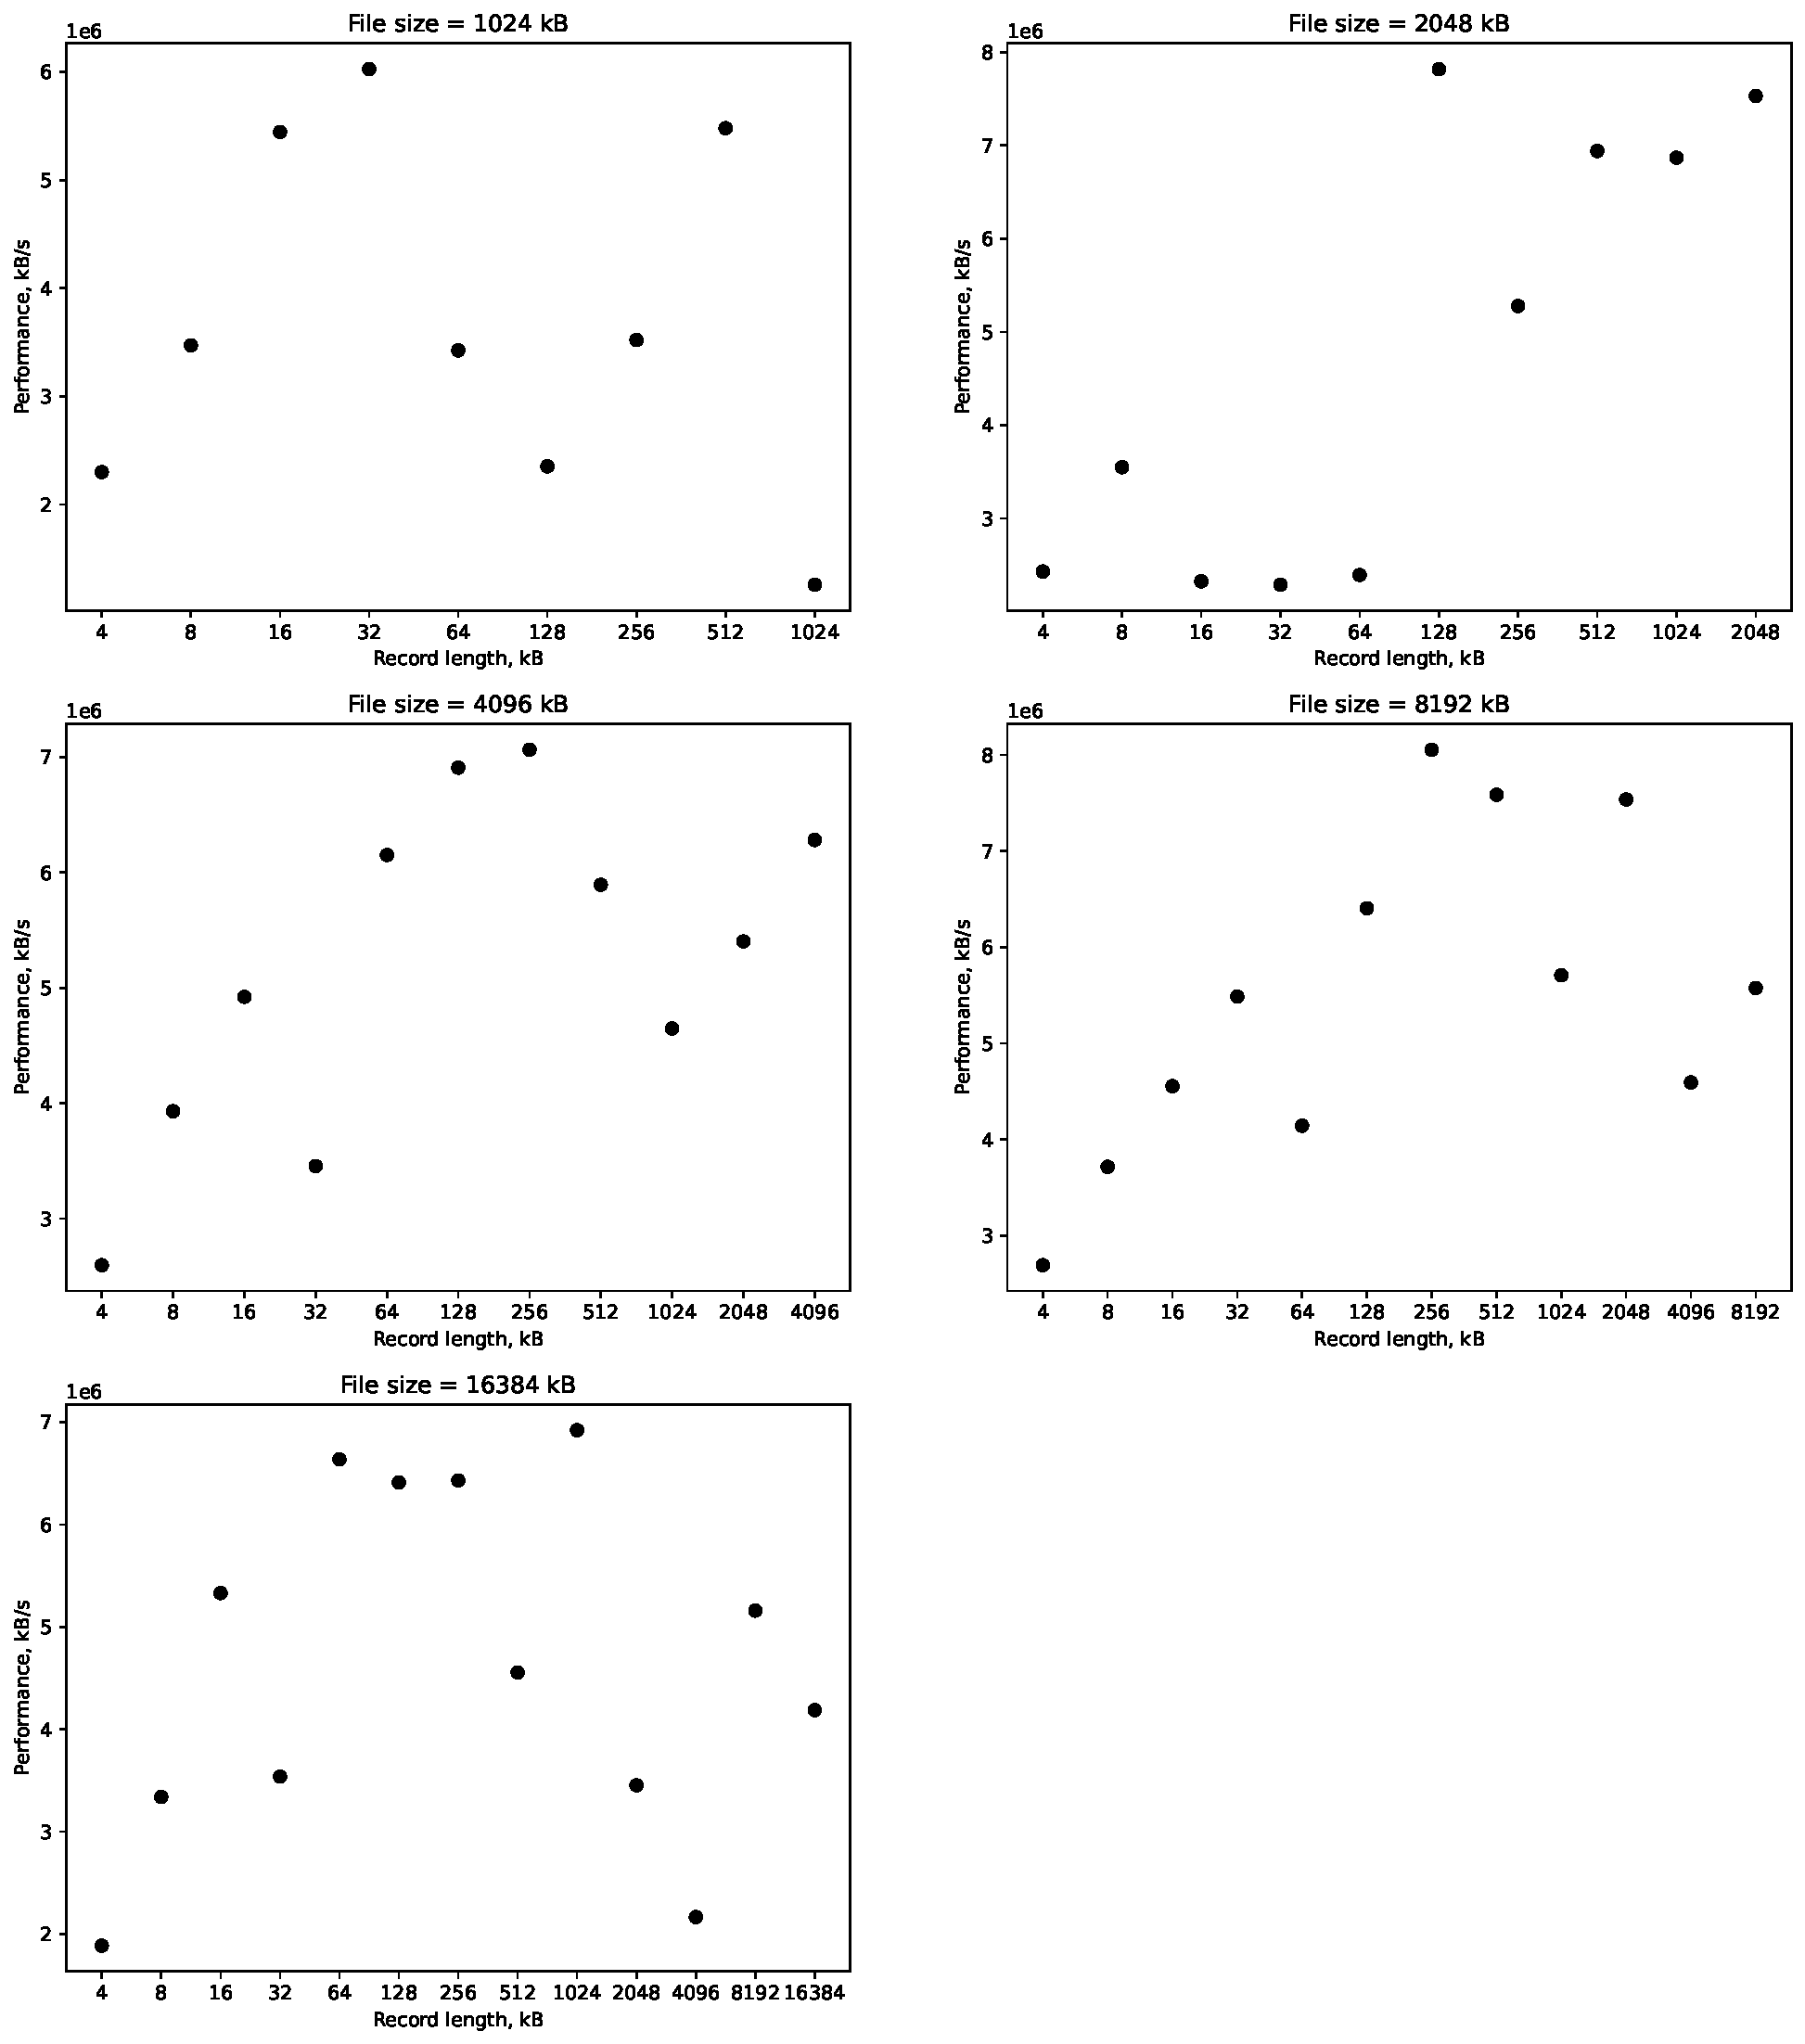
\includegraphics[width=1.0\textwidth]{figures/benchmarking/local/Read.pdf}
	\end{center}
	\caption{IOZone output for APFS Forward Read}
\end{figure}

\begin{figure}[!htb]
	\label{fig:app_benapfsffs_write}
	\begin{center}
		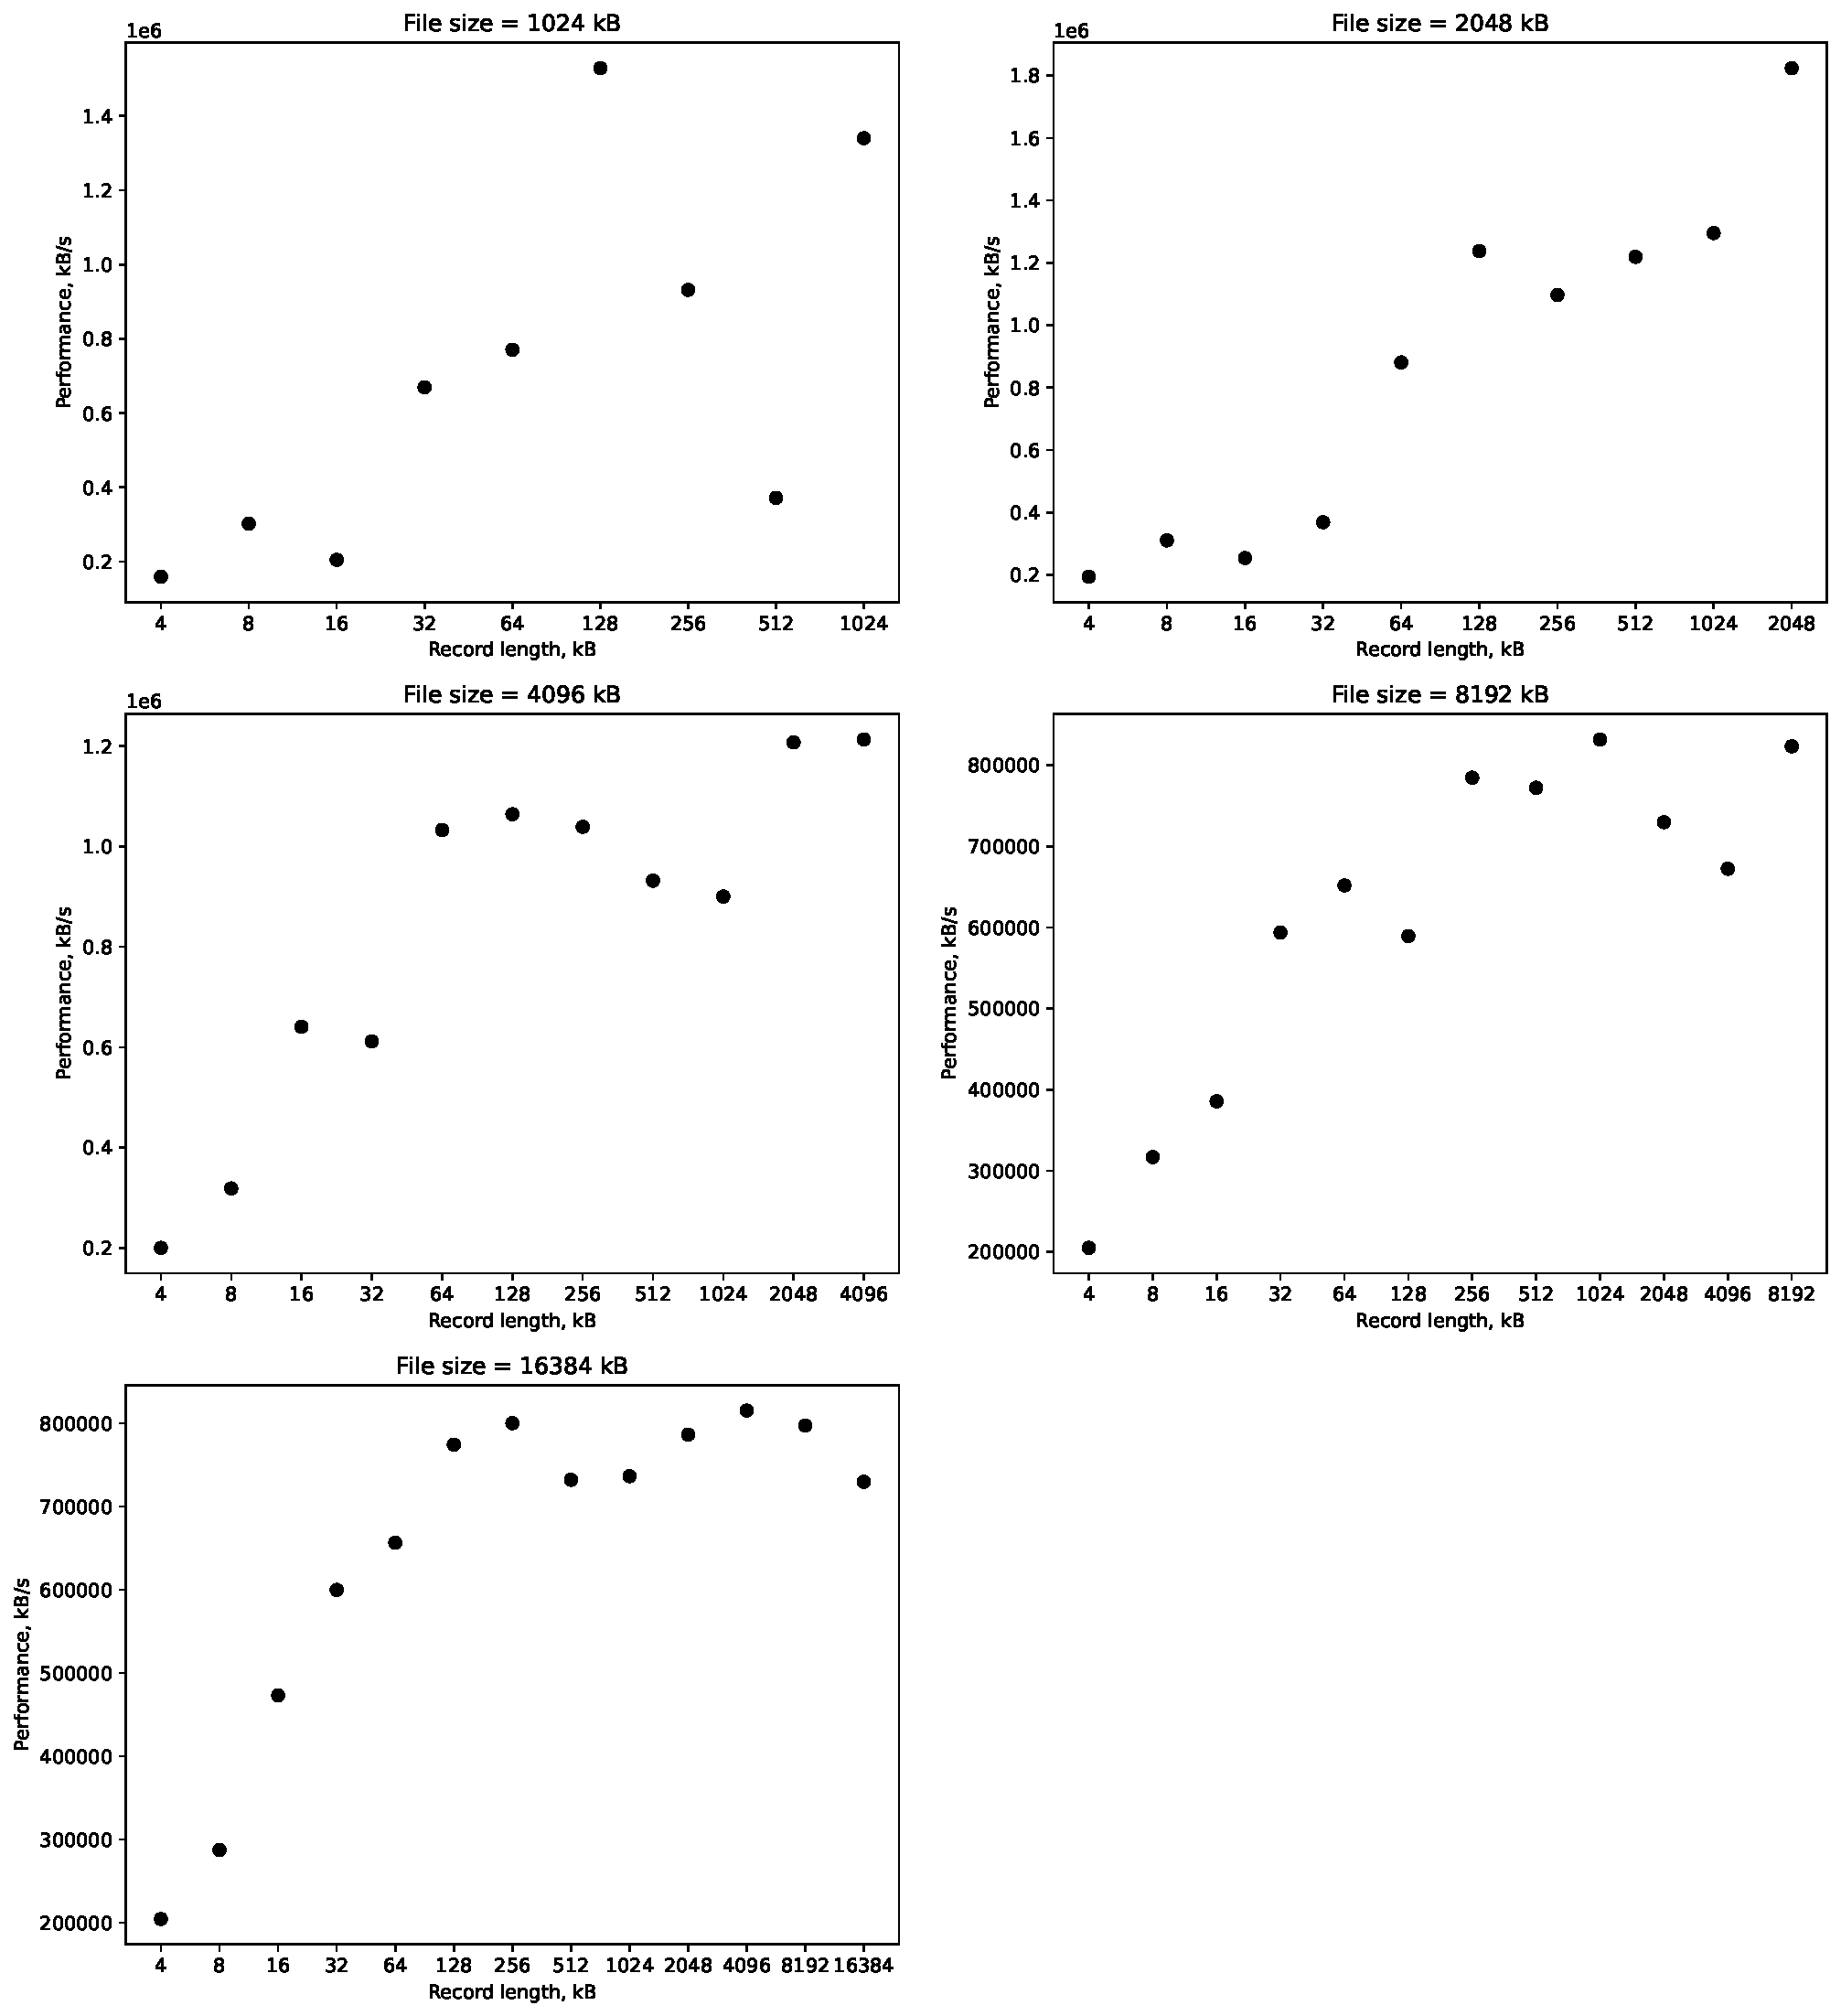
\includegraphics[width=1.0\textwidth]{figures/benchmarking/local/Write.pdf}
	\end{center}
	\caption{IOZone output for APFS Forward Write}
\end{figure}

\begin{figure}[!htb]
	\label{fig:app_benchapfss_re_read}
	\begin{center}
		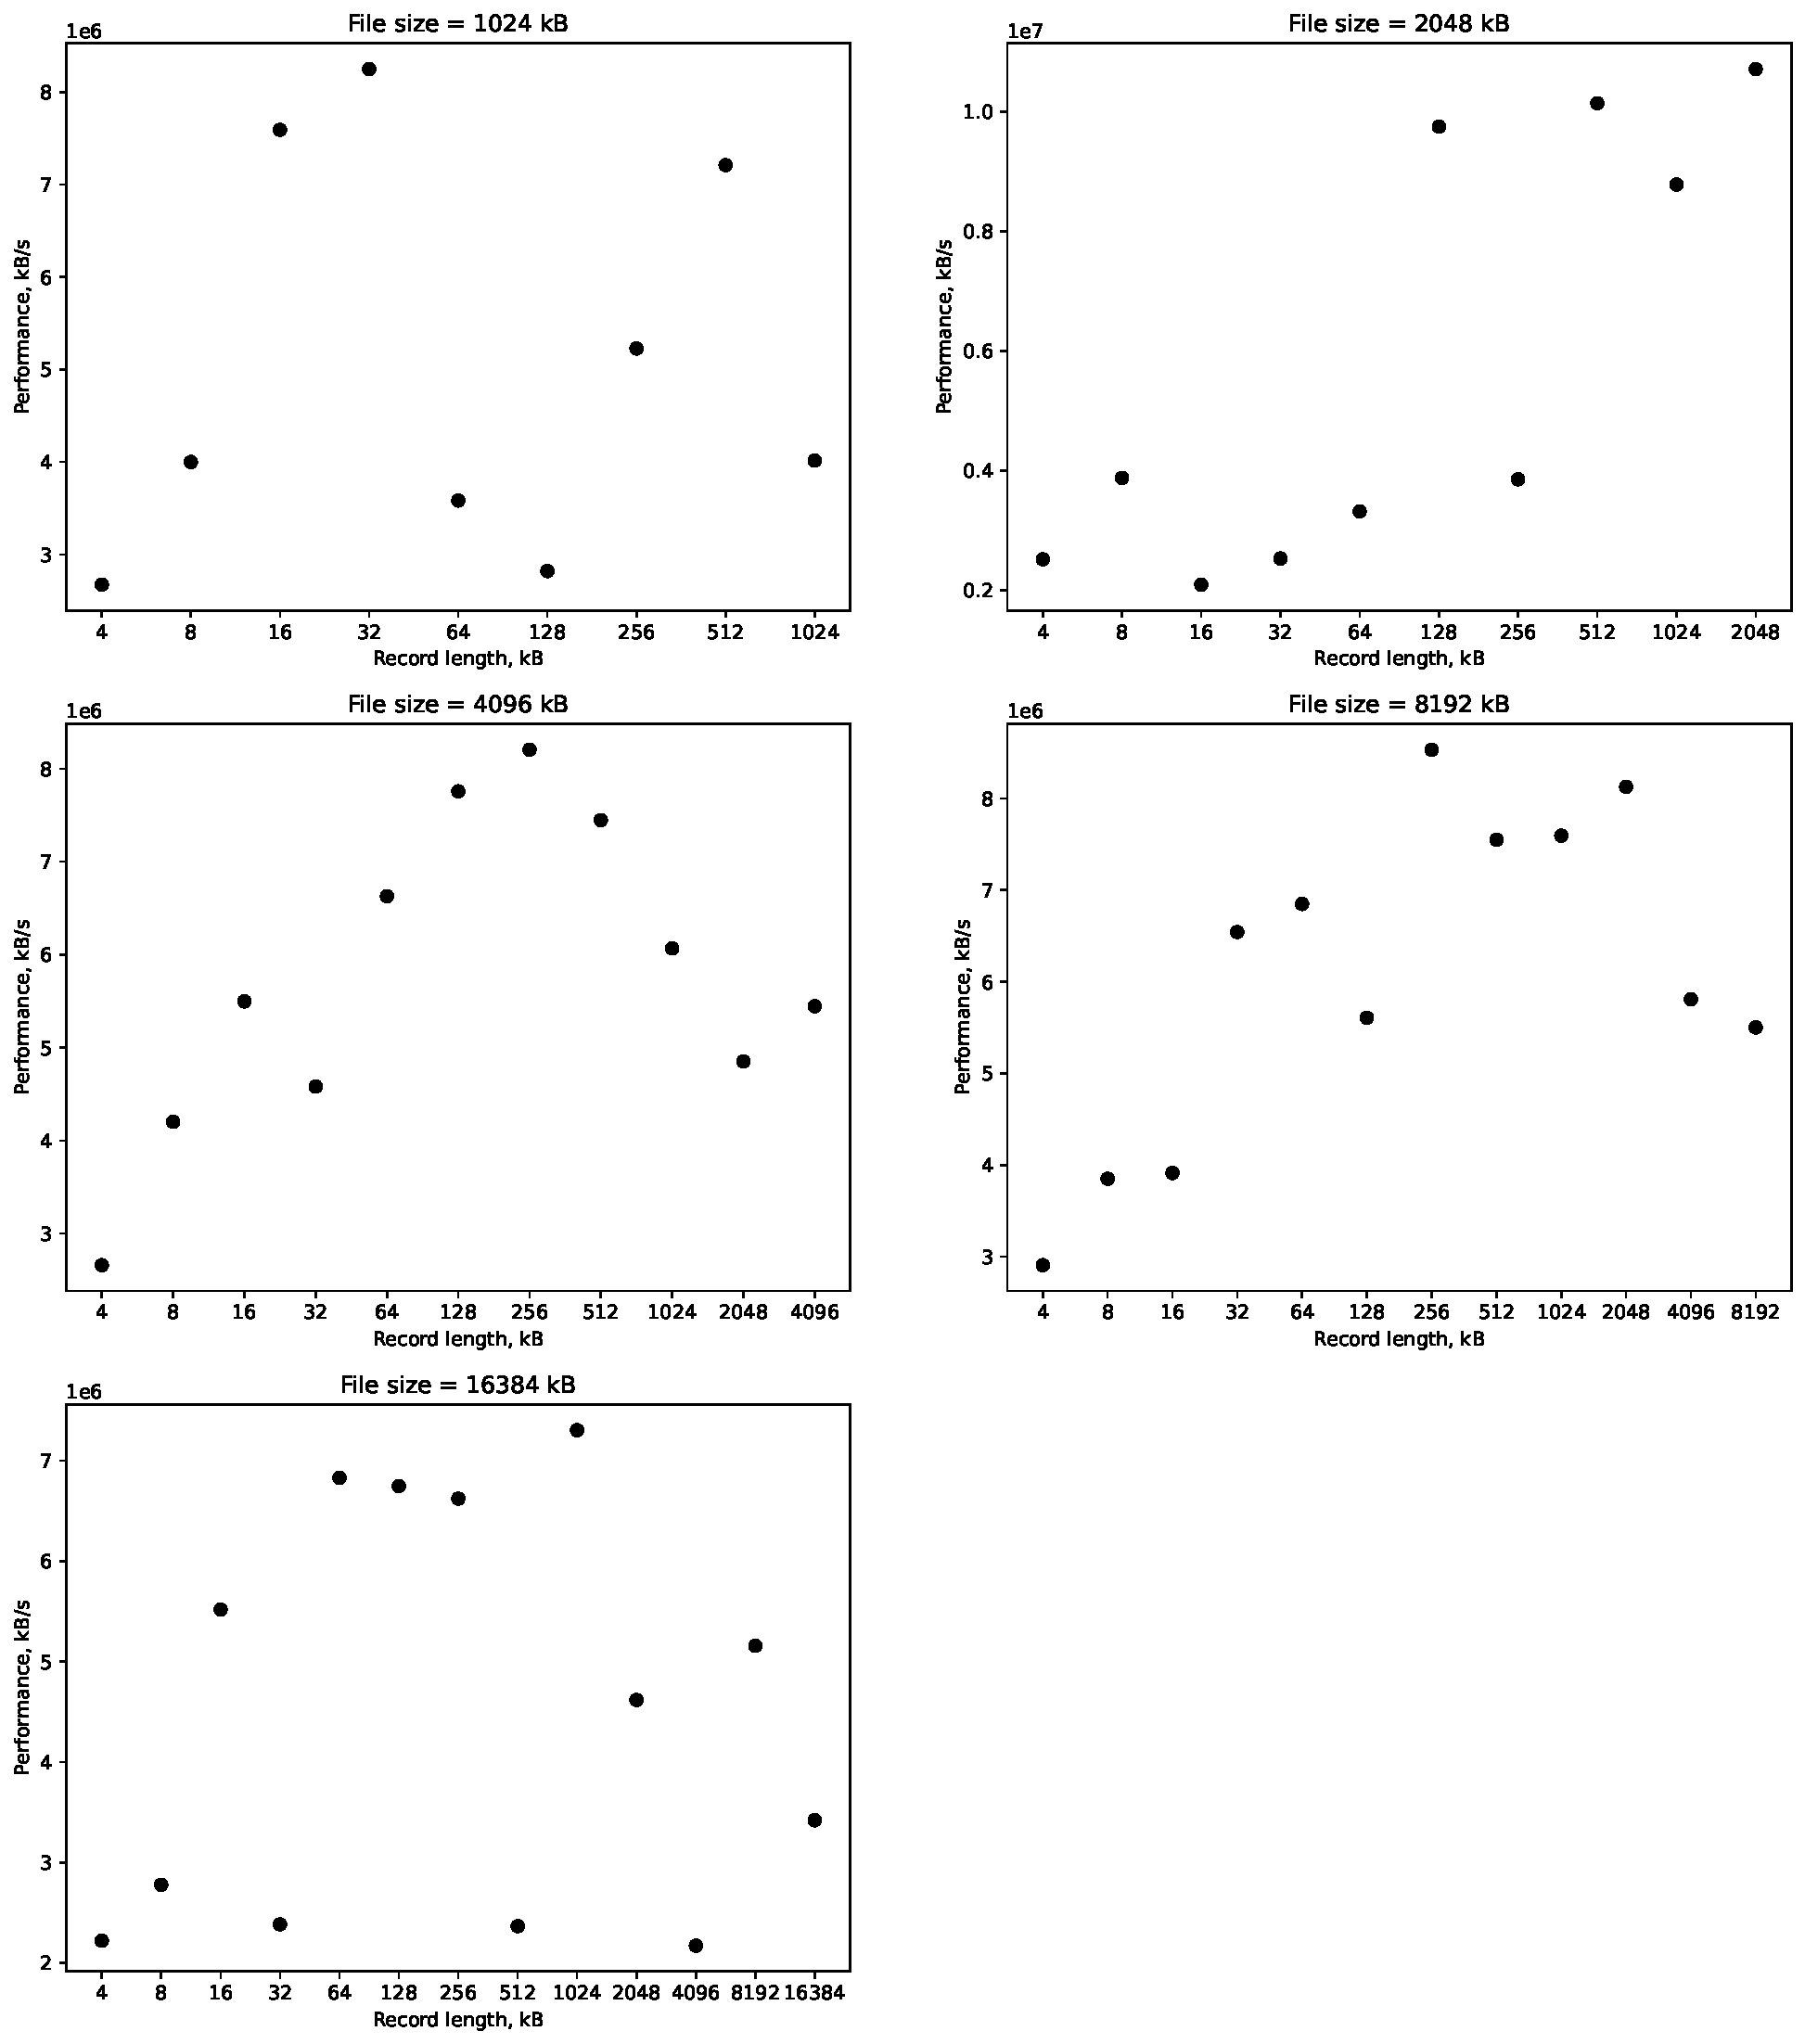
\includegraphics[width=1.0\textwidth]{figures/benchmarking/local/Re-Read.pdf}
	\end{center}
	\caption{IOZone output for APFS Re-Read}
\end{figure}

\begin{figure}[!htb]
	\label{fig:app_bench_apfs_re_write}
	\begin{center}
		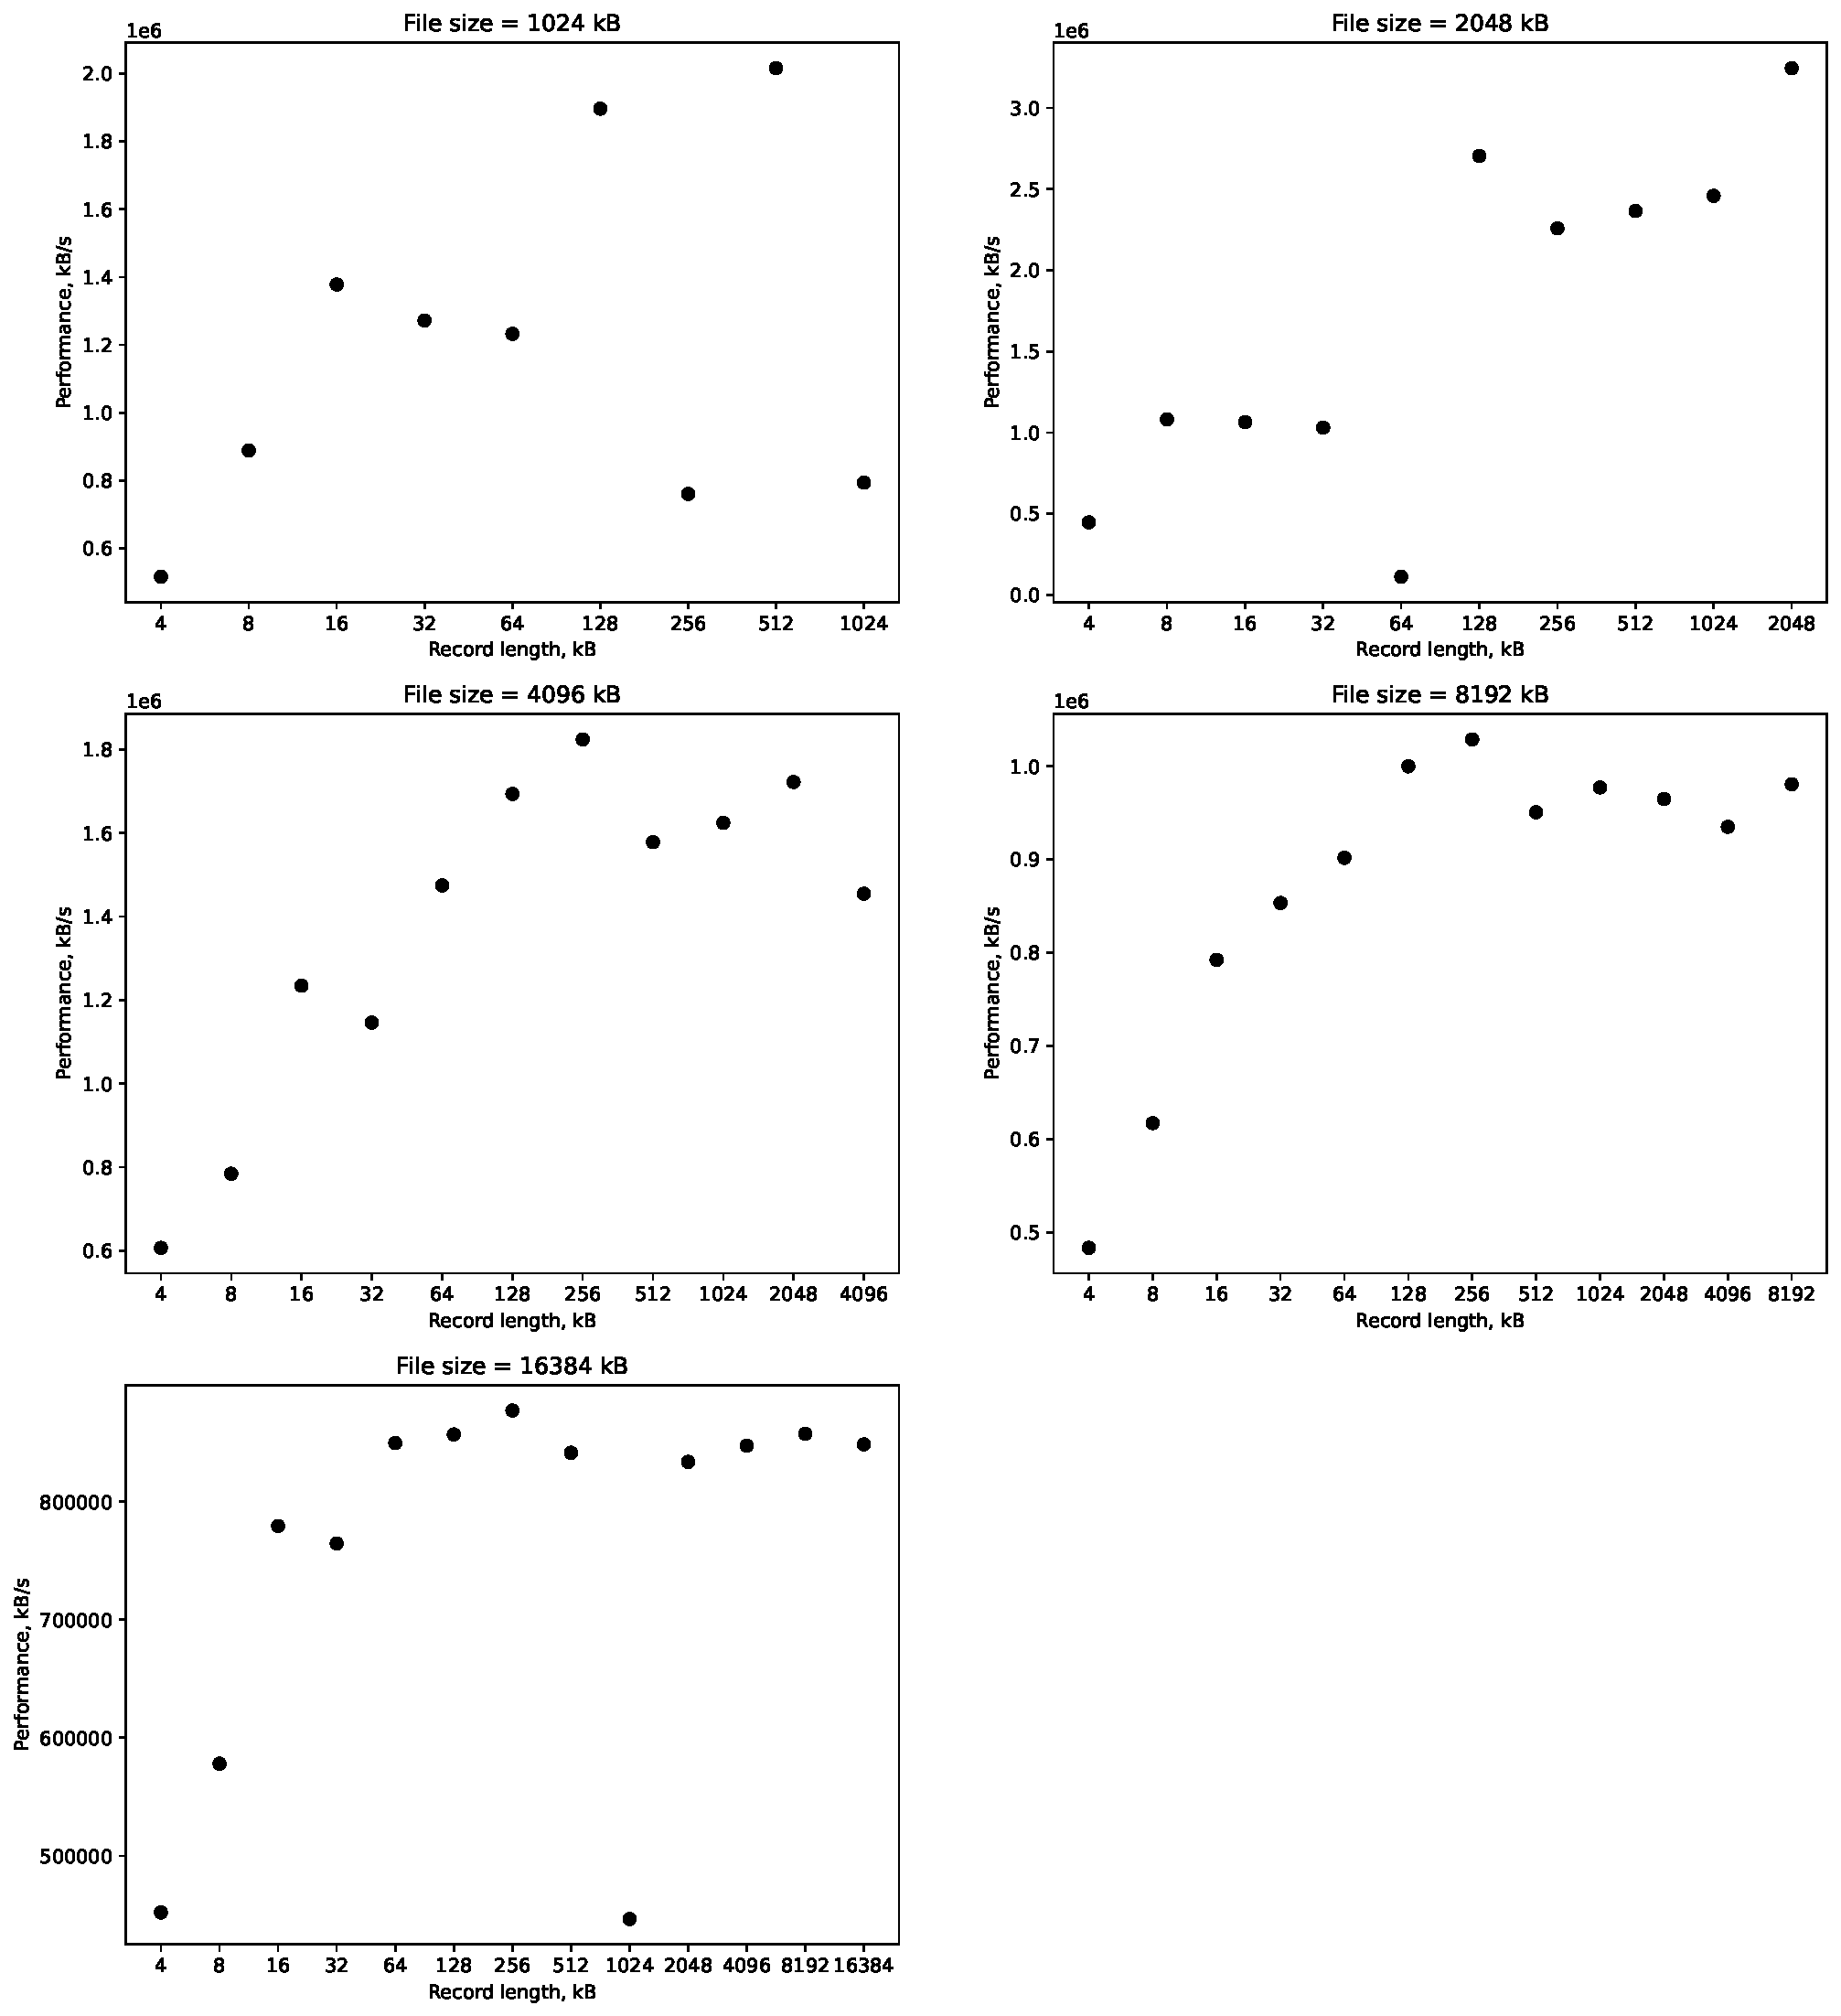
\includegraphics[width=1.0\textwidth]{figures/benchmarking/local/Re-Write.pdf}
	\end{center}
	\caption{IOZone output for APFS Re-Write}
\end{figure}

\begin{figure}[!htb]
	\label{fig:app_bench_apfs_rnd_read}
	\begin{center}
		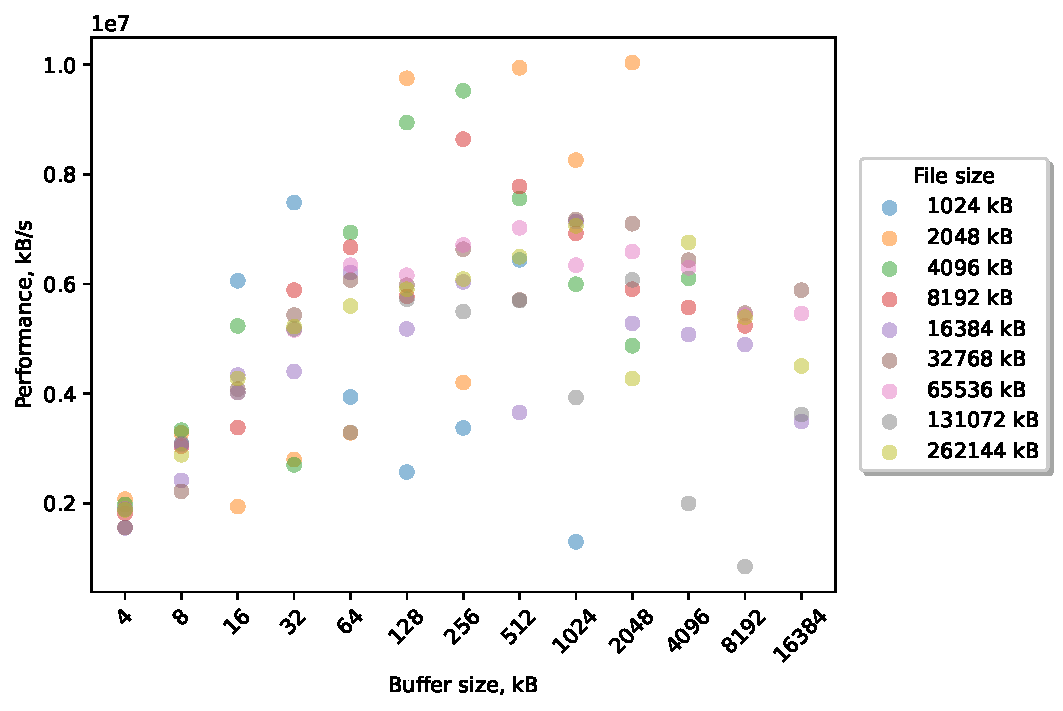
\includegraphics[width=1.0\textwidth]{figures/benchmarking/local/Random read.pdf}
	\end{center}
	\caption{IOZone output for APFS Random read}
\end{figure}

\begin{figure}[!htb]
	\label{fig:app_bench_fapfsrnd_write}
	\begin{center}
		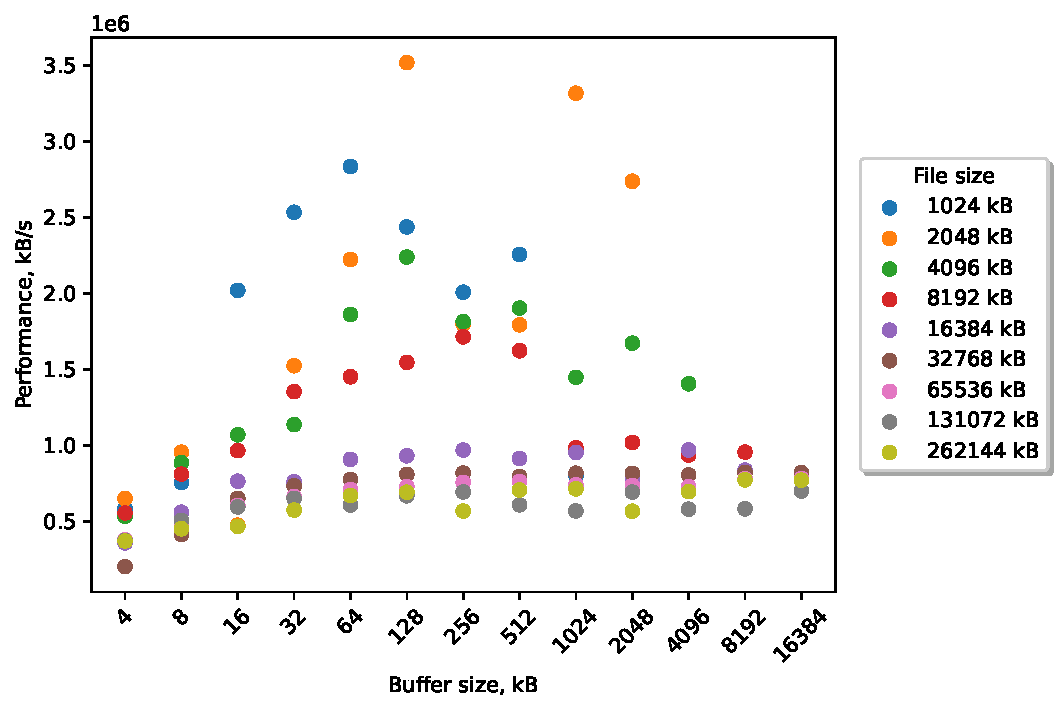
\includegraphics[width=1.0\textwidth]{figures/benchmarking/local/Random write.pdf}
	\end{center}
	\caption{IOZone output for APFS Random write}
\end{figure}